\documentclass[a4paper,11pt]{article}
\usepackage[table]{xcolor}



\newcommand{\defeq}{\mathrel{\doteq}}

\newcommand{\lzero}{0}

\newcommand{\kw}[1]{\mathtt{#1}}

\newcommand{\expr}{e}
\newcommand{\vall}{w}
\newcommand{\valr}{v}
\newcommand{\eif}{\kw{if}}
\newcommand{\eapp}{\;}
\newcommand{\eprojl}{\kw{fst}}
\newcommand{\eprojr}{\kw{snd}}
%\newcommand{\eprov}[1]{\eta_{#1}}
\newcommand{\etrue}{\kw{true}}
\newcommand{\efalse}{\kw{false}}
\newcommand{\econst}{c}
\newcommand{\eop}{\delta}
\newcommand{\efix}{\mathop{\kw{fix}}}
%\newcommand{\labelA}{\ell}

\newcommand{\tr}{T}
\newcommand{\trift}{\eif^{\kw{t}}}
\newcommand{\triff}{\eif^{\kw{f}}}
\newcommand{\trprojl}{\eprojl}
\newcommand{\trprojr}{\eprojr}
\newcommand{\trtrue}{\etrue}
\newcommand{\trfalse}{\efalse}
\newcommand{\trconst}{\econst}
\newcommand{\trop}{\eop}
\newcommand{\trfix}{\efix}
\newcommand{\trapp}[5]{#1 \; #2 \mathrel{\triangleright} {\efix #3(#4).#5}}

\newcommand{\adap}{\kw{adap}}
\newcommand{\ddep}[1]{\kw{depth}_{#1}}
\newcommand{\nat}{\mathbb{N}}
\newcommand{\natb}{\nat_{\bot}}
\newcommand{\natbi}{\natb^\infty}
\newcommand{\nnatA}{n}
\newcommand{\nnatB}{m}
\newcommand{\nnatbA}{s}
\newcommand{\nnatbB}{t}
\newcommand{\nnatbiA}{q}
\newcommand{\nnatbiB}{r}

\newcommand{\type}{\tau}
\newcommand{\tbase}{\kw{b}}
\newcommand{\tbool}{\kw{bool}}
\newcommand{\tarr}[5]{#1; #3 \xrightarrow{#4; \, #5} #2}
\newcommand{\env}{\theta}

\newcommand{\bigstep}{\mathrel{\Downarrow}}

\newcommand{\dmap}{\rho}
\newcommand{\dmapb}{\bot_\dmap}
\newcommand{\supp}{\kw{supp}}
\newcommand{\dom}{\kw{dom}}

\newcommand{\tvdash}[1]{\vdash_{#1}}

%Packages
\usepackage[T1]{fontenc}
\usepackage{fourier} 
\usepackage[english]{babel} 
\usepackage{amsmath,amsfonts} 
\usepackage{amsthm} 
\usepackage{color}   %May be necessary if you want to color links
\usepackage{hyperref}
\usepackage{lscape}
\usepackage{geometry}
\usepackage{amsmath}
\usepackage{algorithm}
\usepackage{algorithmic}
\usepackage{amssymb}
\usepackage{amsfonts}
\usepackage{times}
\usepackage{bm}
\usepackage{ stmaryrd }
\SetSymbolFont{stmry}{bold}{U}{stmry}{m}{n}

\usepackage{ amssymb }
\usepackage{ textcomp }
\usepackage[normalem]{ulem}
% For derivation rules
\usepackage{mathpartir}
\usepackage{color}
\usepackage{a4wide}
\usepackage{caption}
\usepackage{subcaption}
\usepackage{mathpartir}
\usepackage{amsmath,amsfonts}
\usepackage{ amssymb }
\usepackage{color}
\usepackage{algorithm}
\usepackage{algorithmic}
\usepackage{microtype}
\usepackage{eucal}
\usepackage{url}
\usepackage{xspace}
\usepackage{array}
\usepackage{listings}

\usepackage{tikz}
\usetikzlibrary{shapes.geometric}
\usetikzlibrary{arrows.meta,arrows}
\usetikzlibrary{decorations.text}
% % % % 


\usepackage{multirow}


%%%%%%%%%%%%%%%%%%%%%%%%%%%%%%%%%%%%%%%%%%%%%%%%%%%%%Packages And Definitions For Listing the Code%%%%%%%%%%%%%%%%%%%%%%%%%%%%%%%%%%%%%%%%%%%%%%%%%%%%%%%%%%%%%%%%%%%%%%%%
\usepackage{listings}
\usepackage{xcolor}

\definecolor{codegreen}{rgb}{0,0.6,0}
\definecolor{codegray}{rgb}{0.5,0.5,0.5}
\definecolor{codepurple}{rgb}{0.58,0,0.82}
\definecolor{backcolour}{rgb}{0.95,0.95,0.92}

\lstdefinestyle{mystyle}{
    backgroundcolor=\color{backcolour},   
    commentstyle=\color{codegreen},
    keywordstyle=\color{magenta},
    numberstyle=\tiny\color{codegray},
    stringstyle=\color{codepurple},
    basicstyle=\ttfamily\footnotesize,
    breakatwhitespace=false,         
    breaklines=true,                 
    captionpos=b,                    
    keepspaces=true,                 
    numbers=left,                    
    numbersep=5pt,                  
    showspaces=false,                
    showstringspaces=false,
    showtabs=false,                  
    tabsize=2
}

\lstset{style=mystyle}

\usepackage{tikz}
\usetikzlibrary{shapes,arrows}
\newcommand{\THESYSTEM}{\textsf{AdaptFun}}

% Define block styles
\tikzstyle{decision} = [diamond, draw, fill=blue!20, 
    text width=4.5em, text badly centered, node distance=3cm, inner sep=0pt]
\tikzstyle{block} = [rectangle, draw, fill=blue!20, 
    text width=5em, text centered, rounded corners, minimum height=4em]
\tikzstyle{line} = [draw, -latex']
\tikzstyle{cloud} = [draw, ellipse,fill=red!20, node distance=3cm,
    minimum height=2em]

\begin{document}
\title{Appendix for "Program Analysis for Adaptivity Analysis"}

\author{}

\date{}

\maketitle

In this appendix, we present the full details of the 2 languages: while language and the SSA language.

\tableofcontents


% \section{Introduction}
\section{System Overview}


In adaptive data analysis, a data analysis can depend on the results of
previous analysis over the same data. This dependency may affect the
\emph{generalization properties of the data analysis}. To study this phenomenon
in a formal way, we consider the \emph{statistical query
  model}. In this model, a dataset $X$ consisting of $d$ attributes (columns) and $n$
individuals' data (rows) can be accessed only through an interface to
which one can submit statistical queries. More precisely, suppose that
the type of a row is $R$ (as an example, a row with $d$ binary
attributes would have type $R=\{0,1\}^d$. Then, in the statistical
query model one can access the dataset only by submitting a query to
the interface, in
the form of a function
$p:D\to [0,1] $ where $D$ represents dataset. The collected answer of
the asked query is the average result of $p$ on each row in the
dataset $D$. For example, the result is the
value $\frac{1}{n}\sum_{i=1}^n p(X_i)$ where
$X_i$ is the row of index $i$ in $X$. While this model is rather
simple, in fact it supports sufficient statistics one may be
interested.

 

We are interested in the adaptivity of mechanisms in the model, which is straightforward supported by a high level language. In this language, queries are allowed to carry arguments to simulate the process of submitting a query to the interface in
the model, for example, the expression $\query(e)$ tells us the argument $e$ is consumed to construct the
query. To be precise, one submitted query who needs the average of
answers of previous queries is expressed as $\query(x)$, where the variable $x$ stores
the expected average results.This makes these mechanisms quite straightforward to express in the high level language. However, this convenience pays at the price that the adaptivity $A$ of a mechanism $P$ becomes quite tricky to estimate because the definition of dependency between two queries becomes vague in the high level language. 

\[
\begin{array}{l}
     x \leftarrow q_1() ; \\
    \eif \; (x_1 > 0 )\; \\
     y \leftarrow q_2(x) \; \\
\end{array}
\]

The dependency between two query submissions is the essential of the adaptivity of a mechanism. To study the dependency, we first study its dual, independence between two queries, which is defined to be: one query
$q_1$ does not
depend on another query $q_2$ when the result of $q_1$ remains the
same regardless of the modification of the result of $q_2$. Hence, it becomes hard to distinguish whether the variance of result of $q_1$ comes from the control flow or the argument of queries. Since we know that the result of one query from a specific $D$ may vary under different contexts in the high level language.  


To resolve the dilemma, we translate any program(mechanism) into its counterpart in a low level language, which mimics the high level one except its only allowing atomic queries, -- $q$ --. That is to say, given a data base $D$, the result of the
query from $D$ becomes deterministic. We need to show the two programs $P$ and $P^*$ are observably equivalent over the translation. In this way, we can define the adaptivity of
a program under this model only based on the control flow.
To be specific, the adaptivity $A^*$ of a low level program $P^*$ is defined by
graphs, called dependency graph, which comes from the semantics of the low level program. The dependency graph is constructed using a
trace of queries generated along with the semantics: The queries in the trace consists of the nodes in the graph
while the edge represents dependency. If there is no dependency between
two node(queries), there will be no edge. Intuitively, we want to give an over-approximate of $A^*$ by static analysis. To this end, we propose {\THESYSTEM}, which estimates a reasonable upper bound on the arbitrary low level program.

The adaptivity $A$ of arbitrary high level program $P$ is defined to be the minimal of the adaptivity $A^*$ of all the possible $P^*$ via various valid translations. Being valid means the programs before and after the translation are observably equivalent. Naturally, following this definition, the upper bound estimated by {\THESYSTEM} is sound with respect to its low level adaptivity $A^*$, hence the high level one $A$. 


Finally we extend the language to support the probabilistic program and extend the adaptivity definition accordingly.


The key component of the system is an program analysis procedure, which provides an upper bound on the adaptivity of the program.

\section{Label While Language}
\label{sec:while_language}
%
\subsection{Syntax and Semantics}
%
\[
\begin{array}{llll}
 \mbox{Arithmetic Operators} & \oplus_a & ::= & + ~|~ - ~|~ \times 
%
~|~ \div \\  
  \mbox{Boolean Operators} & \oplus_b & ::= & \lor ~|~ \land ~|~ \neg\\
  %
   \mbox{Relational Operators} & \sim & ::= & < ~|~ \leq ~|~ == \\  
   \mbox{Label} & l & \in &  \mathbb{N}  \\  
\mbox{Arithmetic Expressions} & \aexpr & ::= & 
	%
	n ~|~ x ~|~ \aexpr \oplus_a \aexpr ~|~ \\
% \sep \pi (l , \aexpr, \aexpr) \\
    %
\mbox{Boolean Expressions} & \bexpr & ::= & 
	%
	\etrue ~|~ \efalse  ~|~ \neg \bexpr
	 ~|~ \bexpr \oplus_b \bexpr
	%
	~|~ \aexpr \sim \aexpr \\
\mbox{Expressions } & \expr & ::= & \jl{\aexpr \sep \bexpr ~|~ [] ~|~ [\expr, \dots, \expr]} \\
\mbox{Values } & v & ::= & \jl{ n \sep \etrue \sep \efalse ~|~ [] ~|~ [v, \dots, v]}  
\\
\mbox{Query expressions} & \qexpr & ::= 
& \jl{ \aexpr ~|~ \chi ~|~ \chi[\aexpr] ~|~ \qexpr \oplus_a \qexpr} 
\\
\mbox{Query Values} & \qval & ::= 
& \jl{ n ~|~ \chi ~|~ \chi[n] ~|~ \qval \oplus_a  \qval }
\\
\mbox{commands} & c & ::= &   \assign x \expr ~|~  \assign{x}{ \query(\qexpr)}
%
~|~ \\ 
&&&  \jl{\ewhile ~ b ~ \edo ~ c}  ~|~ c;c  ~|~ \eif(\bexpr, c, c) 	 ~|~ \eskip 
	\\
\mbox{Memory} & m & ::= & [] ~|~ m[x \to v] \\
\mbox{Trace} & t & ::= & [] 
~|~ \jl{{( \query(\qval), l, w) :: t}} \\
%
\mbox{Annotated Query} & \mathcal{AQ}  & 
::= & \jl{\{( \query(\qval), l, w) \} } 
\\
%
\mbox{\jl{While Maps}}
& w & ::= & \jl{[] |  w[l \to n]}
\\
%
\mbox{\jl{Query Domain}}
& \qdom & ::= & \jl{[-1,1]}
\end{array}
\]
%
%
\subsection{ Trace-based Operational Semantics}
\jl{
We evaluate programs in our {\tt While} language by means of a trace-based operational semantics, to capture the dependency between queries. For distinguishing elements in the the trace, we add a label to commands in the {\tt While} language as follow:
%
\[
\begin{array}{llll}
     \mbox{Labeled commands} & c & ::= &   [\assign x \expr]^{l} ~|~  [\assign x q(\qexpr)]^{l}
 ~|~  \ewhile ~ [b]^l ~ \edo ~ c  ~|~ c;c  ~|~ \eif([\bexpr]^l, c, c) 	 ~|~ [\eskip]^{l} \\
\end{array}
\]
%
Each command is now labeled with a label $l$, a natural number standing for the line of code where the command appears. Notice that we associate the label $l$ to the conditional predicate $\bexpr$ in the if statement, and to the loop counter $\aexpr$ in the loop statement. We will also use  Loop Maps $w$ as defined below.  
%
\[
	\begin{array}{llll}
	\mbox{While Maps} & w & \in & \mbox{Label} \to \mathbb{N} \\
	 %
	\mbox{Annotated Query} & \mathcal{AQ}  & ::= 
		& \{ (\query(\qval), l, w)   \} \\
	\end{array}
	\begin{array}{llll}
	\mbox{Memory} & m & ::= & [] ~|~ m[x \to v] \\
	\mbox{Trace} & t & ::= 
		& [] ~|~ ( \query(\qval), l, w) :: t \\
	\end{array}
\]
%
  	While maps are map from labels $l$ to iteration number $n$.
%
  	A mapping $[k \to n]$ gives accurate information on which while loop the statement is in by finding its corresponding label $k$, (also the key in the map). The label $k$ specifies the line number of the conditional of the while loop the current statement lives. And the mapped result $n$ indicates the iteration number the current statement belongs to. For example, the loop maps $w=[3:1, 4:2]$ indicates that the statement is currently in a nested loop, the outer while loop starting from label $3$ (where the outside conditional is) and in its first iteration, the statement is now in the inner loop starting from label $4$ and in the second iteration. We use $\emptyset$ to represent an empty map, indicating the statement is not in any loop. We define operations on $w$ as follows.
  	%
  	\jl{
	\[
	\begin{array}{lll}
	w \setminus l     & = w  & l \not\in Keys(w)   \\
	     & = w' & w = w' [l \to \_] \\
	w + l & = w[l \to 0] & l \not \in Keys(w) \\   
	     & = w'[l \to n+1] &  w = w'[l \to n]
	\end{array}
	\]
	}
%
  	We use $w \setminus l$ to remove the mapping of the key $l$ from the loop maps $w$. This is used when exiting the loop at line $l$. The special loop maps $w_l$ expresses a map identical to $w$, but without the mapping of label $l$. We record in $w$ the first iteration of a loop marked by label $l$ by assigning $l$ with the iteration $1$. The mapped number increase when going into another iteration of the same loop. We use $Keys(w)$ to return all the keys of the while maps $w$.
}

\jl{
	%%% trace, queries
	A memory is standard, a map from variables to values. Queries can be uniquely annotated as $\mathcal{AQ}$, and the annotation $(l,w)$ considers the location of the query by line number $l$ and which iteration the query is at when it appears in a loop statement, specified by $w$. A trace $t$ is a list of annotated queries accumulated along the execution of the program. 
	}

\jl{	 
	 %% trace
	A trace can be regarded as the program history, where this history consists of the queries asked by the analyst during the execution of the program. We collect the trace with a trace-based small-step operational semantics based on transitions of the form $ \config{m,c, t, w} \to \config{m', \eskip, t', w'} $. 
	It states that a configuration $\config{m, c, t,w}$ evaluates to another configuration with the trace and loop maps updated along with the evaluation of the command $c$ to the normal form of the command $\eskip$.  
	A configuration contains four elements: a memory $m$, the command $c$ to be evaluated, a starting trace $t$, a starting loop maps $w$. Most of the time, the loop maps remains empty until the evaluation goes into loops.  
	We also have the evaluation of arithmetic expressions of the form $\config{m,\aexpr} \aarrow \aexpr' $, evaluating an arithmetic expression $\aexpr$ in the memory $m$, and similar for the boolean expressions $\config{m, \bexpr} \barrow \bexpr'$.  
  }

{
\begin{figure}
\begin{mathpar}
	\boxed{ \config{m,\aexpr} \aarrow \aexpr' \, : \, Memory  \times AExpr \Rightarrow AExpr }
	\\
	\inferrule{ 
	  \config{m, \aexpr} \aarrow \aexpr'
	}{
	 \config{m,  \chi( \aexpr)} \aarrow \chi(\aexpr')
	}
	\\
	\boxed{ \config{m, \bexpr} \barrow \bexpr' \, : \, Memory \times BExpr \Rightarrow BExpr }
	\end{mathpar}
	\begin{mathpar}
	\boxed{ \config{m, c, t,w} \xrightarrow{} \config{m', c',  t', w'} \; }
	\\
	\inferrule
	{
	 \config{m, \expr } \xrightarrow{}  \config{m, \expr' }
	}
	{
	\config{m, [\assign x \expr]^{l},  t, w} \xrightarrow{} \config{m, [\assign x \expr']^{l}, t, w}
	}
	~\textbf{assn1}
	%
	~~~~~~
	%
	\inferrule
	{
	}
	{
	\config{m, [\assign x v]^{l},  t, w} \xrightarrow{} \config{m[v/x], [\eskip]^{l}, t, w}
	}
	~\textbf{assn2}
	%
	\and
	%
	\jl{
	{\inferrule
	{
	 \empty
	}
	{
	\config{m, \ewhile ~ [b]^{l} ~ \edo ~ c, t, w }
	\xrightarrow{} 
	\config{
	m, c ; 
	\eif_w (b, c ; 
	\ewhile ~ [b]^{l} ~ \edo ~ c,  \eskip),
	t, w
	}
	}
	~\textbf{while-b}
	}
	}
	%
	\and
	%
	\jl{{\inferrule
	{
	 m, b \xrightarrow{} b'
	}
	{
	\config{m, 
	\eif_w (b, c, \eskip) ,  
	t, w }
	\xrightarrow{} \config{m, 
	 \eif_w (b', c,  \eskip), t, w }
	}
	~\textbf{ifw-b}
	}
	}
	%
	\and
	%
	\jl{{
	\inferrule
	{
	 \empty
	}
	{
	\config{m, 
	\eif_w (b, 
	c ; \ewhile ~ [b]^{l} ~ \edo ~ c, 
	\eskip),
	t, w }
	\xrightarrow{} 
	\config{m, 
	c ; \ewhile ~ [b]^{l} ~ \edo ~ c,  
	t, {(w + l)} }
	}
	~\textbf{ifw-true}
	}
	}
	\and
	%
	\jl{{
	\inferrule
	{
	 \empty
	}
	{
	\config{
	m, 
	\eif_w (\efalse, c; \ewhile ~ [b]^{l} ~ \edo ~ c,\eskip), 
	t, w 
	}
	\xrightarrow{} \config{m, 
	 \eskip, t, (w \setminus l) }
	}
	~\textbf{ifw-false}
	}
	}
	%
	\and
	%
	\jl{
	\inferrule
	{
	\config{m,\qexpr} \qarrow \config{m,\qexpr'}
	}
	{
	\config{m, [\assign{x}{\query(\qexpr)}]^l, t, w} \xrightarrow{}  
	\config{m, [\assign{x}{\query(\qexpr')}]^l, t, w}
	}
	~\textbf{query-e}
	}
	\and
	\jl{
	\inferrule
	{
	\query(\qval) = v
	}
	{
	\config{m, [\assign{x}{\query(\qval)}]^l, t, w} 
	\xrightarrow{} 
	\config{m[ v/ x], \eskip,  (\query(\qval), l, w) :: t,w }
	}
	~\textbf{query-v}
	}
	%
	\and
	%
	%
	\inferrule
	{
	\config{m, c_1,  t,w} \xrightarrow{} \config{m', c_1',  t',w'}
	}
	{
	\config{m, c_1; c_2,  t,w} \xrightarrow{} \config{m', c_1'; c_2, t',w'}
	}
	~\textbf{seq1}
	%
	\and
	%
	\inferrule
	{
	}
	{
	\config{m, [\eskip]^{l} ; c_2,  t,w} \xrightarrow{} \config{m, c_2,  t,w}
	}
	~\textbf{seq2}
	\and
	%
	\inferrule
	{
	\config{ m, \bexpr} \barrow \bexpr'
	}
	{
	\config{m, \eif([\bexpr]^{l}, c_1, c_2),  t,w} 
	\xrightarrow{} \config{m,  \eif([\bexpr']^{l}, c_1, c_2),  t,w}
	}
	~\textbf{if}
	%
	\and
	%
	\inferrule
	{
	}
	{
	\config{m, \eif([\etrue]^{l}, c_1, c_2),t,w} 
	\xrightarrow{} \config{m, c_1,  t,w}
	}
	~\textbf{if-t}
	%
	~~~~~~
	%
	\inferrule
	{
	}
	{
	\config{m,  \eif([\efalse]^{l}, c_1, c_2),  t,w} 
	\xrightarrow{} \config{m, c_2,  t,w}
	}
	~\textbf{if-f}
	%
	%
	\end{mathpar}
	    \caption{Trace-based operational semantics of while language.}
    	\label{fig:evaluation}
	\end{figure}
	}
	%
%
\jl{
We define rules of the trace-based operational semantics in Figure~\ref{fig:evaluation}.
The rule $\textbf{query-e}$ evaluates the argument of a query request. When the argument is in normal form, this query will be answered.
%
The rule $\textbf{query-v}$ modifies the starting memory $m$ to $m[v_q/x]$ using the answer $v_q$ of the query $q(v)$ from the mechanism, with the trace expanded by appending the query $q(v)$ with the current annotation $(l,w)$. 
%
The rule for assignment is standard and the trace remains unchanged.%
The sequence rule keeps tracking the modification of the trace, and the evaluation rule for if conditional goes into one branch based on the result of the conditional predicate $\bexpr$. 
%
The rules for while modify the while maps $w$. 
In the rule $\textbf{ifw-true}$, the while maps $w$ is updated by $w + l$ because the execution goes into another iteration when the condition $n >0$ is satisfied. 
%
When $n$ reaches $0$, the loop exits and the while maps $w$ eliminates the label $l$ of this while statement by $w \setminus l$ in the rule $\textbf{ifw-false}$.  
}   
%
\jl{
\subsection{ Query-based Dependency Graph}
%
We define adaptivity through a query-based dependency graph. In our model, an \emph{analyst} asks a sequence of queries to the mechanism, and the analyst receives the answers to these queries from the mechanism. A query is adaptively chosen by the analyst when the choice of this query is affected by answers from previous queries. In this model, the adaptivity we are interested in is the length of the longest sequence of such adaptively chosen queries, among all the queries the data analyst asks to the mechanism.  Also, when the analyst asks a query, the only information the analyst will have will be the answers to previous queries and the state of the program. It means that when we want to know if this query is adaptively chosen, we only need to check whether the choice of this query will be affected by changes of answers to previous queries. There are two possible situations that can  affect the choice of a query,  
either the query argument directly uses the results of previous queries (data dependency), or the control flow of the program with respect to a query (whether to ask this query or not) depends on the results of previous queries (control flow dependency).
}

\jl{
As a first step, we give a definition of when one query may depend on a previous query, which is supposed to consider both control dependency and data dependency. We first look at two possible candidates:
\begin{enumerate}
    \item One query may depend on a previous query if and only if a change of the answer to the previous query may also change the result of the query.
    \item One query may depend on a previous query if and only if a change of the answer to the previous query may also change the appearance of the query.
\end{enumerate}
}

\jl{
   The first candidate works well by witnessing the result of one query according to the change of the answer of another query. We can easily find that the two queries have nothing to do with each other in a simple example   
%
    $ p = \assign{x}{q(\chi(1))} ; \assign{y}{q(\chi(2))}$. This candidate definition works well with respect to data dependency. However, if fails to handle control dependency since it just monitors the changes to the answer of a query when the answer of previous queries returned change. The key point is that this query may also not be asked because of an analyst decision which depend on the answers of previous queries. An example of this situation is shown in program $p_1$ as follows.
    \[
      p_1 = \assign{x}{q(\chi(1))} ; \eif( x > 2 ,\assign{y}{q(\chi(2))}, \eskip )
   	\]
	%   
   	We choose the second candidate, which performs well by witnessing the appearance of one query $q(\chi(2))$ upon the change of the result of one previous query $q(\chi(1))$ in $p_1$. It considers the control dependency, and at the same, does not miss the data dependency. In particular, the arguments of a query characterizes it. In this sense, if the data used in the arguments changes due to a different answer to a certain previous query, the appearance of the query may change as well. This situation is also captured by our definition. Let us look at another variant of program $p$, $p_2$, in which the queries equipped with functions using previously assigned variables storing answer of its previous query.
    \[
      p_2 = \assign{x}{q(\chi(2))} ; \assign{y}{q(x+\chi(3))}
   	\]
    As a reminder, in the {\tt Loop} language, the query request is composed by two components: a symbol $q$ representing a linear query type and the argument $\expr$, which represents the function specifying what the query asks. So we do think $q(\chi(1))$ is different from $q(\chi(2))$. Informally, we think $q(x+\chi(3))$ may depend on the query $q(\chi(2))$, because equipped function of the former $x+\chi(3)$ depend on the data assigned with $q(\chi(2))$. We can see the appearance definition catches data dependency in such a way, since $q(x+\chi(2))$ will not be the same query if the value of $x$ is changed.    
}

\jl{
   We give a formal definition of query may dependency based on the trace-based operational semantics as follows.
   }
   %
%
\begin{defn}[Label Order]
$<_w and =_w$.\\
\[
  \begin{array}{lll}
     w_1 =_w w_2  &  \triangleq &  Keys(w_1) = Keys(w_2) \land \forall k \in Keys(w_1). w_1(k) = w_2(k) \\
     \emptyset =_w \emptyset & &   \\
  \end{array}
\] 
$mk(w_i) =MinKey(w_i) $ 
\[
\begin{array}{lllr}
     w_1 <_w w_2 & \triangleq & & w_1 = \emptyset \\
     & \triangleq  & mk(w_1) < mk(w_2) & w_1,w_2 != \emptyset  \\
     & \triangleq & w_1(mk(w_1)) < w_2(mk(w_2))   & mk(w_1) = mk(w_2) \\
     & \triangleq & (w_1 \setminus mk(w_1) ) <_w (w_2 \setminus mk(w_2)) & Otherwise
\end{array}
\]
\end{defn}
%
\begin{defn}[Query Direction]
Direction between two queries.
\\
\jl{
$\forall \query(\qval_1), \query(\qval_2), l_1, l_2, w_1, w_2 $.
the execution of annotated query $( \query(\qval_1), l_1, w_1)$ appears before annotated query $( \query(\qval_2), l_2, w_2)$, denoted as
%
\[
\mathsf{To}((\query(\qval_1), l_1, w_1), ( \query(\qval_2), l_2, w_2))
= 
(\query(\qval_1), l_1, w_1) 
<_q ( \query(\qval_2), l_2, w_2)
\]
where \\
\[
(\query(\qval_1), l_1, w_1) 
<_q ( \query(\qval_2), l_2, w_2)
 \triangleq 
 \left\{
 \begin{array}{ll}
    l_1 < l_2  
    & w_1=\emptyset \lor w_2 = \emptyset \lor w_1 =_w w_2
    \\
    w_1 <_w w_2
    & \mathsf{Otherwise}
\end{array}  
\right.
\]
}
\end{defn}
%
%
\begin{defn}
Query may dependency.
\\
\jl{
One annotated query $({\alpha}_1, l_1, w_1)$ may depend on another query $({\alpha}_2,l_2, w_2)$ in a program $c$, with a starting memory $m$ and  hidden database $D$, denoted as 
%
$\mathsf{DEP}({(\alpha_1, l_1, w_1)}, ({\alpha}_2, l_2, w_2), c, m, D)$ is defined below. 
}
\jl{
\[
\begin{array}{l}
\exists m_1,m_3,t_1,t_3,c_2,v_1.\\
  \left (\begin{array}{l}   
\config{m, c, \emptyset ,\emptyset} \rightarrow^{*} 
\config{m_1, [\assign{x}{\query({\alpha}_1)}]^{l_1} ; c_2,
  t_1, w_1} 
\rightarrow^{\textbf{query-v}} 
\\ 
\config{m_1[v_1/x], c_2,
(\query({\alpha}_1),l_1, w_1)::t_1, w_1} \rightarrow^{*} \config{m_3, \eskip,
t_3,w_3}
  % 
 \\ \land
  \left( 
  \begin{array}{l}
  (\query({\alpha}_2),l_2,w_2) \in_{q} (t_3-t_1) 
  % 
  \\
  \implies 
  \exists v \in \qdom, v \neq v_1, m_3', t_3', w_3'. ~  
  \config{m_1[v/x], {c_2}, (\query({\alpha}_1),l_1, w_1)::t_1, w_1} 
  \\ 
  \quad \quad 
  \rightarrow^{*}
  (\config{m_3', \eskip, t_3', w_3'} 
  \land 
  (\query({\alpha}_2),l_2,w_2) \not \in_{q} (t_3'-t_1))
\end{array} \right )
\\\land
\left( 
  \begin{array}{l}
	(\query({\qval}_2),l_2,w_2) \not\in_{q} (t_3-t_1)
  	% 
  	\\
  	\implies 
	\exists v \in \qdom, v \neq v_1, m_3', t_3', w_3'. 
	\config{m_1[v/x], {c_2}, (\query({\qval}_1),l_1,w_1)::t_1, w_1}
	\\ 
	\quad \quad 
	\rightarrow^{*} 
	(\config{m_3', \eskip, t_3', w_3'} 
	\land 
	(\query({\qval}_2),l_2,w_2))  \in_{q} (t_3'-t_1))
\end{array} \right )
\end{array} \right )
\end{array}
\]
}
\end{defn}
%
%
\begin{defn}
Trace-based Dependency Graph
\\
 \jl{
Given a program $c$, a database $D$, a starting memory $m$, the trace-based dependency graph $G(c,D,m) = (V, E)$ is defined as: 
\\
$V =\{({\qval}, l,w) \in \mathcal{AQ} \mid 
\exists m',  w', t'.  
\config{m ,c, \emptyset, \emptyset}  
\to^{*}  
\config{m' , \eskip, t', w' }  
\land (\query({\qval}), l, w) \in t'  \}$.
\\
$E = \left\{(({\qval},l,w),({\qval}',l',w')) \in \mathcal{AQ} \times \mathcal{AQ} 
~ \left \vert ~ 
\mathsf{DEP}((({\qval}'),l',w'),({\qval},l,w)),c,m,D)
 \right.\right\}$.
 }
\end{defn}
The edge is directed, when an annotated query $(\query({\qval}),l,w)$ may depend on its previous query $(\query({\qval}'),l',w')$, we have the directed
edge $(({\qval},l,w), ({\qval}',l'.w'))$, 
from vertex $(\qval,l,w) $ to vertex $({\qval}',l'.w')$.
%
%
\begin{defn}
Adaptivity from a trace-based dependency graph.
\\
\jl{
Given a program $c$, and a memory $m$, a database $D$, 
the adaptivity of the trace-based dependency graph $G(c,D,m) = (V, E)$ is the length of the longest path in the graph. 
We denote the path from vertex $({\qval},l,w)$ to vertex $({\qval}',l',w')$ as $p(({\qval},l,w),({\qval}',l',w'))$. 
%
$$
A(c, D, m) = 
\max\limits_{({\qval},l,w),({\qval}',l',w') \in V }
\{ |p(({\qval},l,w),({\qval}',l',w'))| \}
$$
}
\end{defn}
%
We proved some useful properties for our language.
\begin{lem}
[Trace Non-Decreasing].
\\
\jl{
for any program $c$ with a tarting memory $m$, trace $t$ and while label $w$, if 
$  
\config{m, c, t, w} 
\rightarrow^{*} 
\config{m, c', t', w'} 
$ by the operational semantics, then we have
\[
	t' \geq t
\]
}
\end{lem}
%
\begin{proof}
\jl{
Proof is obvious by induction on the operational semantics rules.
}
\end{proof}
%
\begin{lem}
[Semi-Determinism].
\\
\jl{
for any program $c$ with a tarting memory $m$, trace $t$ and while label $w$, 
if program $c$ contains neither  
$[\assign{x}{\query(\qexpr)}]^l$ nor $[\assign{x}{\query(\qval)}]^l$ for any $\qexpr$ and $\qval$, then
%
$$
\bigwedge
\left\{\begin{array}{l}
\config{m, c, t, w} 
\rightarrow^{*} 
\config{m_1, \eskip, t_1, w_1} 
\\ 
\config{m, c, t, w} 
\rightarrow^{*} 
\config{m_2, \eskip, t_2, w_2} 
\end{array}
\right\}
\implies
(m_1 = m_2 \land t_1 = t_2 \land w_1 = w_2)
 $$ 
}
\end{lem}
%
\begin{proof}
\jl{
Proof is obvious by induction on the operational semantics rules.
}
\end{proof}
%
%
The evaluation of the query expression is deterministic while the evaluation of the query itself can be non-deterministic. Below the Lemma Query Non-Determinism formally described this property. 
%
\begin{lem}
[Query Semi-Determinism].
\\
\jl{
Given a program $c; \assign{x}{\query(\qexpr)}; c'$ with a starting memory $m$, trace $t$ and while label $w$, 
s.t. $c$ contains neither  
$[\assign{x}{\query(\qexpr)}]^l$ nor $[\assign{x}{\query(\qval)}]^l$ for any $\qexpr$ and $\qval$, 
we have the Semi-Determinism property as follows:
%
\[
\bigwedge
\left\{
\begin{array}{l}
\config{m, c; \assign{x}{\query(\qexpr)}; c', t, w} 
\rightarrow^{*} 
\config{m_1, \assign{x}{\query(\qval_1)}; c', t_1, w_1} 
\\
\config{m, c; \assign{x}{\query(\qexpr)}; c', t, w} 
\rightarrow^{*} 
\config{m_2, \assign{x}{\query(\qval_2)}; c', t_2, w_2} 
\end{array}
\right\}
\implies
(\qval_1 = \qval_2 \land m_1 = m_2 \land t_1 = t_2 \land w_1 = w_2)
\]
}
\end{lem}
%
\begin{proof}
\jl{
Proof is obvious by induction on the operational semantics rules.
}
\end{proof}
%
%
\begin{lem}
[Adaptivity Toplimit].
\\
\jl{
Given a program $c$ with a database $D$ and a tarting memory $m$,
the top limitation for $A(c, D, m)$ as follows:
%
\[
\config{m, c, \emptyset, \emptyset} 
\rightarrow^{*} 
\config{m', \eskip, t', w'} 
\implies
A(c, D, m) \leq |t'|
\]
}
\end{lem}
%
\begin{proof}
\jl{
Proof is obvious by induction on the operational semantics rules.
}
\end{proof}
%
%
\clearpage

\section{SSA-form language  }
%
\jl{
\subsection{The limit of loop language for analysis}
we see the power of the labelled loop language to achieve the adaptivity semantically, from its being capable to express many adaptive data analysis algorithm,  allowing the construction of the query-based dependency graph using traces from the execution, and so on.
However, it is not powerful enough to reach the adaptivity syntactically. The main difficulty is its implicit control flow which raises extra complexity to figure out where some variables used come from. We use three simple but relevant examples to show why the loop language suffers. We use $\query(0),\query(1)$ to represent linear queries.
%
\[
 s_1 = \begin{array}{l}
      \clabel{ \assign{x}{\query(0)}}^{1} ; \\
      \eif  [(x < 0 )]^{2} \\
      \ethen \clabel{\assign{x}{\query(1)}}^{3}\\
      \eelse \clabel{\eskip}^{4} ; \\
      \clabel{\assign{y}{\query(x+\chi(3))}}^{5}
 \end{array}
 ~~~~~
  s_2 = \begin{array}{l}
      \clabel{ \assign{x}{\query(0)}}^{1} ; \\
      \eif  [(x < 0 )]^{2} \\
      \ethen \clabel{\assign{x}{\query(1)}}^{3}\\
      \eelse \clabel{\assign{x}{\query(2)}}^{4} ; \\
      \clabel{\assign{y}{\query(x+\chi(3))}}^{5}
 \end{array}
 ~~~~~~~~
  s_3 = \begin{array}{l}
      \clabel{ \assign{x}{\query(0)}}^{1} ; \\
      \eif  [(x < 0 )]^{2} \\
      \ethen \clabel{\assign{z}{\query(1)}}^{3}\\
      \eelse \clabel{\eskip}^{4} ; \\
      \clabel{\assign{y}{\query(x+\chi(3)}}^{5}
 \end{array}
\]
In these three examples, the variable $x$ at line $5$ is implicit. In program $s_1$, it refers to the either $x$ at line $1$, or $x$ at line $3$, which means the result of query request $q(x+\chi(3))$ assigned to the variable $y$ may depend on $\query(0)$(bound to $x$ at line $1$) or $\query(1)$($x$ at line $3$). When we have a look at the other two programs $s_2$ and $s_3$, it is another talk. We think $\query(x+\chi(3))$ may depend on either $\query(1)$($x$ at line $3$) or $\query(x+\chi(3))$($x$ at line $4$) in $s_2$,     
while $\query(x+\chi(3))$ only depends on $\query(0)$ at line $1$ in program $s_3$. 
These three examples are structural similar in loop language, however, the dependency between variables are quite dissimilar. We consider variables here because query request is also bound to variables. To solve this dilemma, we move to single static assignment as follows.   
\[
 s_1^{s} = \begin{array}{l}
      \clabel{ \assign{{\ssa{x_1}}}{\query(0)}}^{1} ; \\
      \eif  [({\ssa{x_1} }< 0 )]^{2}\\
      ([], [{ \ssa{x_3, x_1,x_2} }], []) \\
      \ethen \clabel{\assign{{\ssa{x_2}}}{\query(1)}}^{3}\\
      \eelse \clabel{\eskip}^{4} ; \\
      \clabel{\assign{{\ssa{y_1}}}{\query({\ssa{x_3} + \chi(3)})}}^{5}
 \end{array}
 ~~~~~
  s_2^{s} = \begin{array}{l}
      \clabel{ \assign{{\ssa{x_1}}}{\query(0)}}^{1} ; \\
      \eif  [({\ssa{x_1}} < 0 )]^{2}, \\
      ( [{\ssa{x_4, x_2,x_3}}], [], [] ) \\
      \ethen \clabel{\assign{{\ssa{x_2}}}{\query(1)}}^{3}\\
      \eelse \clabel{\assign{{\ssa{x_3}}}{\query(2)}}^{4} ; \\
      \clabel{\assign{{\ssa{y_1}}}{\query({\ssa{x_4}}+\chi(3))}}^{5}
 \end{array}
 ~~~~~~~~
  s_3^{s} = \begin{array}{l}
      \clabel{ \assign{{\ssa{x_1}}}{\query(0)}}^{1} ; \\
      \eif  [({\ssa{x_1}} < 0 )]^{2} \\
       ( [], [], [] ) \\
      \ethen \clabel{\assign{{\ssa{z_1}}}{\query(1)}}^{3}\\
      \eelse \clabel{\eskip}^{4} ; \\
      \clabel{\assign{{\ssa{y_1}}}{\query({\ssa{x_1}}+\chi(3))}}^{5}
 \end{array}
\]
To distinguish between the loop language and in ssa form, we denote the ssa variable ${\ssa{x_1}}$ in bold. As we can see, the data flow becomes explicit in ssa form and the analysis on the dependency between variables in the program becomes much clear now. Considering this advantage, we aim to estimate the adaptivity through an analysis on program in ssa form. 
}
%
\subsection{SSA-form While Language}
\[
\begin{array}{llll}
 \mbox{Arithmetic Operators} & \oplus_a & ::= & + ~|~ - ~|~ \times 
%
~|~ \div \\  
  \mbox{Boolean Operators} & \oplus_b & ::= & \lor ~|~ \land ~|~ \neg\\
  %
   \mbox{Relational Operators} & \sim & ::= & < ~|~ \leq ~|~ == \\  
 \mbox{Label} & l & := & \mathbb{N} \\ 
 \mbox{Loop Maps} & w & \in & \mbox{Label} \times \mathbb{N} \\
\mbox{Arithmetic Expressions} & \saexpr & ::= & 
	%
	\textrm{n} ~|~ \textrm{x} ~|~ \saexpr \oplus_a \saexpr  \\
    %
\mbox{Boolean Expressions} & \bexpr & ::= & 
	%
	\textrm{true} ~|~ \textrm{false}  ~|~ \neg \sbexpr
	 ~|~ \sbexpr \oplus_b \sbexpr
	%
	~|~ \saexpr \sim \saexpr 
	\\
\mbox{Query expressions} & \qexpr & ::= 
& \jl{ \aexpr ~|~ \chi ~|~ \chi[\aexpr] ~|~ \qexpr \oplus_a \qexpr} 
\\
\mbox{Query Values} & \qval & ::= 
& \jl{ n ~|~ \chi ~|~ \chi[n] ~|~ \qval \oplus_a  \qval }
\\
\mbox{Expressions} & \sexpr & ::= & \saexpr \sep \sbexpr ~|~ [] ~|~ [\expr, \dots, \expr]
\\	
\mbox{Labelled commands} & \ssa{c} & ::= &   [\assign {\ssa{x}}{ \ssa{\expr}}]^{l} ~|~  [\assign {\ssa{x} } {\ssa{\query(\qexpr)}}]^{l}
%
% ~|~ [\eswitch( \ssa{\expr}, \ssa{x}, \ssa{v_i} \to \ssa{ q_i})]^{l} 
~|~  {\jl{\eifvar(\bar{\ssa{x}}, \bar{\ssa{x}}')}} \\ 
&&& 
\jl{\ewhile ~ [ b ]^{l} , n,
~ 
[\bar{\ssa{x}}, \bar{\ssa{x_1}}, \bar{\ssa{x_2}}] 
~ \edo ~  c }
\\
&&&
~|~ \ssa{c};\ssa{c}  
~|~ [\eif(\sbexpr, [\bar{\ssa{x}}, \bar{\ssa{x_1}}, \bar{\ssa{x_2}}] , \ssa{c}, \ssa{c})]^l 
~|~ [\eskip]^{l} \\
\mbox{Memory} & m & ::= & \emptyset ~|~ \ssa{ ({x^{l}} \to v) :: m } \\
%
\mbox{Trace} & t & ::= & [] ~|~ \ssa{{(\query(\qval), l , w ) :: t}} \\
\mbox{Annotated Query} & \mathcal{AQ}  & 
::= & \jl{\{ (\query(\qval), l , w )  \} }
 \\
\mbox{SSA Variables} & \mathcal{SV}  & ::= & \{ \ssa{x} \} \\
\mbox{Labelled SSA Variables} & \mathcal{LV}  & ::= & \{ \ssa{x}^{(l,w)}  \}
\end{array}
\]
%

\jl{
We use $\ssa{\aexpr}$ to express arithmetic expressions which now contains ssa variable $\ssa{x} \in \mathcal{SV}$, 
and the boolean expression as $\ssa{\bexpr}$. 
%
The ssa expression can be either $\ssa{a}$ and $\ssa{b}$. 
We also have the ssa variables annotated in a similar way as the annotated queries in the loop language, denoted as $\mathcal{LV}$. 
%
The labelled commands $\ssa{c}$ are now in the ssa form. 
% assignment
In the assignment $[\assign {\ssa{x}}{ \ssa{\expr}}]^{l}$,  query request $[\assign {{\ssa{x}} } {q({\ssa{e}})}]^{l}$ , the expression ${\ssa{\expr}}$ is now in the ssa form, similar for the $\ssa{\aexpr}$ in the loop and conditional $\ssa{\bexpr}$ in the if command. 
}

\jl{
% if
The if command now contains the extra part 
$([\bar{\ssa{x}}, \bar{\ssa{x_1}}, \bar{\ssa{x_2}}] , 
[\bar{\ssa{y}}, \bar{\ssa{y_1}}, \bar{\ssa{y_2}}],
[\bar{\ssa{z}}, \bar{\ssa{z_1}}, \bar{\ssa{z_2}}] )$, 
which helps to track the dependency of new assigned variables in both branches($[\bar{\ssa{x}}, \bar{\ssa{x_1}}, \bar{\ssa{x_2}}]$), 
then branch $[\bar{\ssa{y}}, \bar{\ssa{y_1}}, \bar{\ssa{y_2}}]$, 
and else branch $[\bar{\ssa{z}}, \bar{\ssa{z_1}}, \bar{\ssa{z_2}}] $. 
The $\bar{\ssa{x}}$ is a list of ssa variables, in which every element $\ssa{x}$ may depends on the corresponding element $\ssa{x_1}$ from $\bar{\ssa{x_1}}$ collected in the then branch or the corresponding element $\ssa{x_2}$ from $\bar{\ssa{x_2}}$ collected in the else branch. 
%
Every tuple $(\ssa{x,x_1,x_2 })$ from $[\bar{\ssa{x}}, \bar{\ssa{x_1}}, \bar{\ssa{x_2}}]$ can be understood as $\ssa{x} = \phi(\ssa{x_1,x_2})$ in the normal ssa form. 
The previous example $s_2^{s}$ can be used for reference. 
The second part $[\bar{\ssa{y}}, \bar{\ssa{y_1}}, \bar{\ssa{y_2}}]$ focuses on the then branch. 
The list of ssa variables $y_1$ stores the assigned ssa variables before the if command, whose non-ssa version (variables in the loo language) will be modified only in the then branch. 
We can look at program $s_1$ as a reference,in which $x$ at line $1$ may be modified only in the then branch at line $3$. 
The list $\bar{\ssa{y_2}}$ tracks the ssa variables assigned only in the then branch. 
If the variables are assigned in both branches such as in the program $s_2$, they goes into $[\bar{\ssa{x}}, \bar{\ssa{x_1}}, \bar{\ssa{x_2}}]$. Then we think every ssa variable in $\bar{\ssa{y}}$ may come from the corresponding variable $\ssa{y_1}$ in $\bar{\ssa{y_1}}$ before the if command or $\ssa{y_2}$ in $\bar{\ssa{y_2}}$ in the then branch. 
In this sense, we can also regard every tuple $(\ssa{y,y_1,y_2 })$ from $[\bar{\ssa{y}}, \bar{\ssa{y_1}}, \bar{\ssa{y_2}}]$ as $\ssa{y} = \phi(\ssa{y_1,y_2})$. 
The rest part $[\bar{\ssa{z}}, \bar{\ssa{z_1}}, \bar{\ssa{z_2}}]$ focus on the else branch and can be understood similarly. 
}

\jl{
% while
Also, the while command also has similar part $ [\bar{\ssa{x}}, \bar{\ssa{x_1}}, \bar{\ssa{x_2}}]$, focusing on the while body. 
The new command ${{\eifvar(\bar{\ssa{x}}, \bar{\ssa{x}}')}}$ does not have explicit label because it is only used for evaluation internally, we will discuss more about it when used in the operational semantics for the ssa loop language. 
The ssa memory $\ssa{m}$ is a map from ssa variable $\ssa{x}$ to values.
}
%
%
\jl{
\subsection{Trace-based Operational Semantics of SSA Loop Language}
When switching to the SSA loop language, we show that we are still able to achieve what we can get in Section~\ref{sec:while_language}. The operational semantics of the SSA loop language mimics its counterpart, of the form $\config{\ssa{m}, \ssa{c}, t, w} \to \config{\ssa{m'}, \eskip, t', w'}$. The SSA memory $\ssa{m}$ is a map from SSA variable $\ssa{x}$ to values. It still uses a trace to track the query requests during the execution, starting from an SSA configuration with SSA memory $\ssa{m}$ and program in its SSA form $\ssa{c}$, which allows a similar construction of the query-based dependency graph in the SSA language as in the {\tt Loop} language.
We show the evaluation rules in Figure~\ref{fig:ssa_evaluation}.
}
%
The command 
$\mathsf{\eifvar}(\bar{x},\bar{x}')$ stores the variable map during the run time, which is a map from ssa variable $\ssa{x}$ to variable $\ssa{x_i}$. This map is designed for if condition, when the variable may comes from two branches and this command records which branch the variable comes from. 
%
\begin{figure}
\begin{mathpar}
\boxed{\config{\ssa{m, a}} \xrightarrow{} \config{\ssa{a}} \;} 
\and
\inferrule{
    \ssa{m}(\ssa{x}) = \ssa{v}
}{ \config{\ssa{m, x }} \to \ssa{v} 
}~{\textbf{ssa-var}}
\\
\boxed{ \config{\ssa{ m, c, t,w}} \xrightarrow{} \config{\ssa{ m', c',  t', w'}} \; }
\and
{ Memory \times Com  \times Trace \times loop maps \Rightarrow^{}  Memory \times Com  \times Trace \times loop maps}
\\
\jl{
	\inferrule
	{
		\ssa{\config{m,\qexpr} \qarrow \config{m,\qexpr'}}
	}
	{
	\config{\ssa{
		m, [\assign{x}{\query(\qexpr)}]^l, t, w} }
	\xrightarrow{} 
	\config{\ssa{
		m, [\assign{x}{\query(\qexpr')}]^l, t, w
	}}
	}
	~\textbf{ssa-query-e}}
%
\and
\inferrule
{
\jl{
\ssa{\query(\qval)(D) = v}}
}
{
\config{\ssa{
m, [\assign{\ssa{x}}{\ssa{\query(\qval)}}]^l, t, w
}} 
\xrightarrow{} 
\config{\ssa{  m[  x \mapsto v], \eskip,  
\jl{\query(\qval),l,w )::t,w }}
}
}
~\textbf{ssa-query-v}
%
\and
%
\inferrule
{
}
{
\config{\ssa{ m, [\assign x v]^{l},  t,w} } \xrightarrow{} \config{\ssa{m[x \mapsto v], [\eskip]^{l}, t,w} }
}
~\textbf{ssa-assn}
%
\and
%
\inferrule
{
\config{ \ssa{m, \bexpr}} \barrow \ssa{\bexpr'}
}
{
\config {\ssa{m, [\eif(\bexpr, [\bar{{x}}, \bar{{x_1}}, \bar{{x_2}}] ,[\bar{\ssa{y}}, \bar{\ssa{y_1}}, \bar{\ssa{y_2}}] ,[\bar{\ssa{z}},\bar{\ssa{z_1}}, \bar{\ssa{z_2}}] , c_1, c_2)]^{l},  t,w} } 
\xrightarrow{} \config{ \ssa{ m,  [\eif(\sbexpr',[ \bar{{x}}, \bar{{x_1}}, \bar{{x_2}}] ,[\bar{\ssa{y}}, \bar{\ssa{y_1}}, \bar{\ssa{y_2}}] ,[\bar{\ssa{z}},\bar{\ssa{z_1}}, \bar{\ssa{z_2}}] , c_1, c_2)]^{l},  t, w} }
}
~\textbf{ssa-if}
%
\and
%
\inferrule
{
}
{
\config{\ssa{m, [\eif(\etrue, [\bar{\ssa{x}}, \bar{\ssa{x_1}}, \bar{\ssa{x_2}}] ,[\bar{\ssa{y}}, \bar{\ssa{y_1}}, \bar{\ssa{y_2}}] ,[\bar{\ssa{z}}, \bar{\ssa{z_1}}, \bar{\ssa{z_2}}] , c_1, c_2)]^{l},t,w}} 
\xrightarrow{} \config{m, c_1; { \ \eifvar(\bar{\ssa{x}},\bar{\ssa{x_1}}); \eifvar(\bar{\ssa{y}},\bar{\ssa{y_2}});\eifvar(\bar{\ssa{z}},\bar{\ssa{z_1}}) }  ,  t,w}
}
~\textbf{ssa-if-t}
%
\and
%
\inferrule
{
}
{
\config{\ssa{m, [\eif(\efalse, [\bar{\ssa{x}}, \bar{\ssa{x_1}}, \bar{\ssa{x_2}}] ,[\bar{\ssa{y}}, \bar{\ssa{y_1}}, \bar{\ssa{y_2}}] ,[\bar{\ssa{z}},\bar{\ssa{z_1}}, \bar{\ssa{z_2}}] , c_1, c_2)]^{l},t,w}} 
\xrightarrow{} \config{m, c_2 ; { \eifvar(\bar{\ssa{x}},\bar{\ssa{x_2}}); \eifvar(\bar{\ssa{y}},\bar{\ssa{y_1}});\eifvar(\bar{\ssa{z}},\bar{\ssa{z_2}}) },  t,w}
}
~\textbf{ssa-if-f}
%
\and
%
\inferrule{
}{
 \config{ \ssa{m,} \eifvar(\ssa{\bar{x}, \bar{x}'}),\ssa{ t,w }} \to \config{ \ssa{m [\bar{x} \to m(\bar{x}')], \eskip , t,w }  }
}~\textbf{ssa-\eifvar}
% %
%
\and
%
%
{
{\inferrule
{
 {n = 0 \rightarrow i = 1 }
 \and
 {n > 0 \rightarrow i = 2 }
}
{
\config{
\ssa{m},  
\ssa{
\ewhile ~ 
[\bexpr]^{l}, n, [\bar{{x}}', \bar{{x_1}}, \bar{{x_2}}] 
~ \edo ~ {c} 
}, t, w 
}
\xrightarrow{} 
\\ 
\config{\ssa{m},
\eif_w (\ssa{
b[\bar{x_i}/\bar{x'}],  [\bar{{x}}', \bar{{x_1}}, \bar{{x_2}}], n, 
c[\bar{x_i}/\bar{x'}] 
}; 
\ssa{
\ewhile ~ 
[b]^{l}, n+1, 
[\bar{{x}}', \bar{{x_1}}, \bar{{x_2}}]  
~ \edo ~ c} ,  
\eskip),
t, w 
}
}
~\textbf{ssa-while-b}
}
}
%
\and
%
{{\inferrule
{
 \ssa{m, b \xrightarrow{} b'}
}
{
\config{\ssa{m, \eif_w (b, [\bar{{x}}', \bar{{x_1}}, \bar{{x_2}}] , n,  c_1,  c_2)} ,  t, w }
\xrightarrow{} \config{\ssa{ m, 
 \eif_w (b', [\bar{{x}}', \bar{{x_1}}, \bar{{x_2}}] , n , c_1 , c_2 )}, t, w }
}
~\textbf{ssa-ifw-b}
}
}
%
\and
%
{
\inferrule
{
 \empty
}
{
\config{
\ssa{
m, 
\jl{
\eif_w (\etrue, [\bar{{x}}', \bar{{x_1}}, \bar{{x_2}}], n,  
c; \ssa{\ewhile ~ [b]^{l}, n, [\bar{{x}}', \bar{{x_1}}, \bar{{x_2}}]  ~ \edo ~ c},
\eskip)
} 
},  t, w 
}
\\
\xrightarrow{} 
\config{
\ssa{m, 
\jl{
\eif_w (\etrue, [\bar{{x}}', \bar{{x_1}}, \bar{{x_2}}], n,  
c; \ssa{\ewhile ~ [b]^{l}, n, [\bar{{x}}', \bar{{x_1}}, \bar{{x_2}}]  ~ \edo ~ c},
}
}
t, (w + l) }
}
~\textbf{ssa-ifw-true}
}
\and
%
{{
\inferrule
{
 { n = 0 \rightarrow i = 1 }
 \and
 {n > 0 \rightarrow i =2}
}
{
\config{\ssa{
m, \eif_w (
\efalse, [\bar{{x}}', \bar{{x_1}}, \bar{{x_2}}],   n, 
\jl{  
c; \ssa{\ewhile ~ [b]^{l}, n, [\bar{{x}}', \bar{{x_1}}, \bar{{x_2}}]  ~ \edo ~ c},
\eskip)
} 
)} ,  t, w }
\\
\xrightarrow{} 
\config{\ssa{m, 
\jl{\eskip}; \eifvar(\bar{x'}, \bar{x_i}) }, t, (w \setminus l) }
}
~\textbf{ssa-ifw-false}
}
}
\end{mathpar}
    \caption{Operational semantics for the ssa while language}
    \label{fig:ssa_evaluation}
\end{figure}
\begin{defn}
Query may dependency in SSA language.
\\
\jl{
One annotated query $({\alpha}_1, l_1, w_1)$ may depend on another query $({\alpha}_2,l_2, w_2)$ in a program $\ssa{c}$,
with a starting memory $\ssa{m}$ and  hidden database $D$, denoted as 
%
$\mathsf{DEP}_{ssa}({(\alpha_1, l_1, w_1)}, ({\alpha}_2, l_2, w_2), \ssa{c}, \ssa{m}, D)$ is defined below. 
%
%
\[
\begin{array}{l}
\exists \ssa{m}_1,\ssa{m}_3,t_1,t_3,\ssa{c}_2,v_1.\\
  \left (\begin{array}{l}   
\config{\ssa{m}, \ssa{c}, \emptyset ,\emptyset} \rightarrow^{*} 
\config{\ssa{m}_1, [\assign{x}{\query({\alpha}_1)}]^{l_1} ; c_2,
  t_1, w_1} 
\\ 
\rightarrow^{\textbf{{ssa-query-v}}} 
\config{\ssa{m}_1[v_1/x], c_2,
(\query({\alpha}_1),l_1, w_1)::t_1, w_1} \rightarrow^{*} \config{\ssa{m}_3, \eskip,
t_3,w_3}
  % 
 \\ \land
  \left( 
  \begin{array}{l}
  (\query({\alpha}_2),l_2,w_2) \in_{q} (t_3-t_1) 
  % 
  \\
  \implies 
  \exists v \in \qdom, v \neq v_1, \ssa{m}_3', t_3', w_3'. ~  
  \config{\ssa{m}_1[v/x], {\ssa{c}_2}, (\query({\alpha}_1),l_1, w_1)::t_1, w_1} 
  \\ 
  \quad \quad 
  \rightarrow^{*}
  (\config{\ssa{m}_3', \eskip, t_3', w_3'} 
  \land 
  (\query({\alpha}_2),l_2,w_2) \not \in_{q} (t_3'-t_1))
\end{array} \right )
\\\land
\left( 
  \begin{array}{l}
	(\query({\qval}_2),l_2,w_2) \not\in_{q} (t_3-t_1)
  	% 
  	\\
  	\implies 
	\exists v \in \qdom, v \neq v_1, \ssa{m}_3', t_3', w_3'. 
	\config{\ssa{m}_1[v/x], {\ssa{c}_2}, (\query({\qval}_1),l_1,w_1)::t_1, w_1}
	\\ 
	\quad \quad 
	\rightarrow^{*} 
	(\config{\ssa{m}_3', \eskip, t_3', w_3'} 
	\land 
	(\query({\qval}_2),l_2,w_2))  \in_{q} (t_3'-t_1))
\end{array} \right )
\end{array} \right )
\end{array}
\]
}
\end{defn}
%
%
\begin{defn}
SSA-based Dependency Graph.
\\
\jl{
Given a program $\ssa{c}$, a database $D$, a starting memory $\ssa{m}$,
the dependency graph $G_{s}(\ssa{c},D,\ssa{m}) = (V, E)$ is defined as: \\
$V =\{({\qval}, l, w) \in \mathcal{AQ} 
\mid 
\exists \ssa{m'},  w', t'.  
\config{\ssa{m} ,\ssa{c}, \emptyset, \emptyset}  
\to^{*}  
\config{\ssa{m'} , \eskip, t', w' }  
\land (\query({\qval}), l, w) \in {t'}  \}$.
\\
$E = 
\left\{
	(({\qval},l, w), ({\qval}',l',w')) \in \mathcal{AQ} \times \mathcal{AQ}
	\mid 
	\mathsf{DEP_{ssa}}(({\qval}',l',w'),({\qval},l,w)), \ssa{c},w,\ssa{m},D)     
\right\}$.
}
\end{defn}
%
%
\jl{
The key idea underneath the operational semantics is to have the trace and the execution path being constructed in a similar way as in the loop language.
Take the query request as an example, the argument $\ssa{e}$ which contains ssa variables will be evaluated to a value $v$ first before the request is sent to the database in rule $\textbf{ssa-query-arg}$. 
The trace expands in the rule $\textbf{ssa-query}$ likewise in the loop language. 
The query $q$, a primitive symbol representing the abstract query in both the ssa language and  the loop language, makes no difference in the two languages. 
Since we add the extra part $[\bar{\ssa{x}}, \bar{\ssa{x_1}}, \bar{\ssa{x_2}}] ,[\bar{\ssa{y}}, \bar{\ssa{y_1}}, \bar{\ssa{y_2}}] ,[\bar{\ssa{z}},\bar{\ssa{z_1}}, \bar{\ssa{z_2}}]  $ in the if command compared to its counterpart in the while language, 
the rules relevant to the if condition ($\textbf{ssa-if-t}$ and $\textbf{ssa-if-f}$) use the command $ifvar(\ssa{\bar{x}, \bar{x}'})$ to update the ssa memory $\ssa{m}$ with the mapping from the new generated variable $\ssa{x}$ in $\bar{\ssa{x}}$ to the appropriate value $\ssa{m(x')}$ where $\ssa{x'}$ is the corresponding variable w.r.t $\ssa{x}$ in $\bar{\ssa{x'}}$.
%
The rule $\textbf{ssa-ifvar}$ reflects the usage of $\eifvar(\ssa{\bar{x}, \bar{x}'})$.
%
It is easier to understand the usage of $\eifvar(\ssa{\bar{x}, \bar{x}'})$ in the rule $\textbf{ssa-if-t}$ when we think about how ssa works: 
in the ssa form, when a variable to be used may come from two sources (e.g. $\ssa{x_1}$ and $\ssa{x_2}$ in the rule), it generates a new variable $\ssa{x}$, assigning it with $\phi(\ssa{x_1}, \ssa{x_2})$,  and replaces the variable to be used with newly assigned $\ssa{x}$. 
We know that in the future program after the if command, 
only the variables $\bar{\ssa{x}}$ will be available instead of $\bar{\ssa{x_1}}, \bar{\ssa{x_2}}$ from two branches.
For the evaluation of the program after the if command, we need to tell the memory the exact value of the newly generated variable $\ssa{x}$, which is the value stored in $\ssa{x_1}$ when the conditional $\ssa{b}$ is true, 
or the value in $\ssa{x_2}$ when $\ssa{b}$ is false. To this end, the internal command $ifvar(\ssa{\bar{x}, \bar{x}'})$ plays its role. 
For the if rule, w
e need to instantiate the variables from $\bar{\ssa{x}}$ whose values come from two branches, 
$\bar{\ssa{y}}$ whose values from then branch or assignment before the if command, and $\bar{\ssa{z}}$ whose values from else branch or before the if command. 
Correspondingly, we need to have three ifvar commands.   
}

\jl{
	The evaluation of while depends on the while iteration counter $\ssa{n}$ and the guard $\ssa{\bexpr}$. 
	When $\ssa{\bexpr}$ is evaluated to $\etrue$, the while is still executing, and all the variables $\ssa{x}$ in $\bar{\ssa{x}}$ of the loop body $\ssa{c}$ are replaced as the corresponding variables in $\bar{\ssa{x_1}}$ in the first iteration($n=0$), or $\bar{\ssa{x_2}}$ in other iterations($n > 0$). 
	The while turns to an exit when $\ssa{n} > 0$, 
	and the memory $\ssa{m}$ updates the mapping of variables in $\bar{\ssa{x}}$ with $\bar{\ssa{x_1}}$ if the guard $\bexpr$ evaluates to $\efalse$, 
	which means the while body is not executed once. 
	When the while enters the exit after executing the body a few times($n$), the variables in $\bar{\ssa{x}}$ is instantiated with the value from the body $\ssa{m}(\bar{\ssa{x_2}})$. 
}

\jl{
	With the trace-based operational semantics of the ssa language at hand, we are able to provide our query-based dependency graph in the ssa language.
}
%
\begin{defn}
Adaptivity from SSA-based Dependency Graph.
\\
\jl{
Given a program $\ssa{c}$, and a memory $\ssa{m}$, a database $D$, 
the adaptivity of the SSA-based dependency graph 
$G_s(\ssa{c}, D,\ssa{m}) = (V, E)$ is the length of the longest path in the graph. 
We denote the path from vertex $({\qval},l,w)$ to vertex $({\qval}',l',w')$ as $p_s(({\qval},l,w),({\qval}',l',w'))$. 
%
$$
A_s(\ssa{c}, D, \ssa{m}) = 
\max\limits_{({\qval},l,w),({\qval}',l',w') \in V }
\{ |p_s(({\qval},l,w),({\qval}',l',w'))| \}
$$
}
\end{defn}


\begin{thm}[\jl{Graph Equivalence}].
\\
\jl{
Given $\Sigma; \delta ; c \hookrightarrow \ssa{c} ; \delta';\Sigma' $,
$\forall m. m \vDash \delta. \forall \ssa{m}, \ssa{m} \vDash_{ssa} \delta \land m = \delta^{-1}(\ssa{m})$, 
then $G_{low}(c,D,m) = G_{ls}(\ssa{c},D,\ssa{m}) $.
}
\end{thm}
%
\begin{proof}
 The nodes in the two graphs are the same according to soundness of the transformation theorem. We will show that the edges are the same. Unfold the definition of $\mathsf{DEP}$, when we find some $v$ in the codomain of one query that may change the appearance of another query,  we can always show that $v = \ssa{v}$ works for $\mathsf{DEP_s}$ as well. In the other direction, for any $\ssa{v}$ that may change the appearance of another query and lead to a different trace $t_3'$ in the ssa execution, there is the same $v = \ssa{v}$ so that the trace $t_3'$ is generated in the while language execution, according to the transformation theorem.  
\end{proof}

\begin{coro}
\jl{Given $\Sigma; \delta ; c \hookrightarrow \ssa{c} ; \delta';\Sigma' $, 
$\forall m. m \vDash \delta. \forall \ssa{m}, \ssa{m} \vDash_{ssa} \delta \land m = \delta^{-1}(\ssa{m})$, starting with a trace $t$ and loop maps $w$, then 
$A(c,D,m) = A_s(\ssa{c},D,\ssa{m}) $.
}
\end{coro}

\subsection{SSA Transformation}
We use a translation environment $\delta$, to map variables $x$ in the low level language to those $\ssa{x}$ in ssa-form language. We use a name environment denoted as $\Sigma$, a set of ssa variables so we can get a fresh variable by $fresh(\Sigma)$. We define $\delta_1 \bowtie \delta_2 $ in a similar way as
\cite{vekris2016refinement}.
\[ \delta_1 \bowtie \delta_2 = \{ ( x, {\ssa{x_1}, \ssa{x_2}} ) \in \mathcal{VAR} \times \mathcal{SV} \times \mathcal{SV} \mid x \mapsto {\ssa{x_1}} \in \delta_1 , x \mapsto {\ssa{x_2} } \in \delta_2, {\ssa{x_1} \not= {\ssa{x_2} }  }  \} \]
\[ \delta_1 \bowtie \delta_2 / \bar{x} = \{ ( x, {\ssa{x_1}, \ssa{x_2}} ) \in \mathcal{VAR} \times \mathcal{SV} \times \mathcal{SV} \mid x \not\in \bar{x} \land x \mapsto {\ssa{x_1}} \in \delta_1 , x \mapsto {\ssa{x_2} } \in \delta_2, {\ssa{x_1} \not= {\ssa{x_2} }   }  \} \]
We call a list of variables $\bar{x}$.
\[
 [\bar{x}, \bar{\ssa{x_1}}, \bar{\ssa{x_2}}] = \{ (x, x_1,x_2)  | \forall 0 \leq i < |\bar{x}|, x = \bar{x }[i] \land x_1 = \bar{x_1}[i] \land x_2 = \bar{x_2 }[i] \land |\bar{x}| = |\bar{x_1}| = |\bar{x_2}|   \}
\]

\begin{mathpar}
\boxed{ \delta ; e \hookrightarrow \ssa{e} }\\
\inferrule{
}{
 \delta ; x \hookrightarrow \delta(x)
}~{\textbf{S-VAR}}\\
\boxed{ \Sigma; \delta ; c  \hookrightarrow \ssa{c} ; \delta' ; \Sigma' } \\
\inferrule{
  { \delta ; \bexpr \hookrightarrow \ssa{\bexpr} }
  \and
  { \Sigma; \delta ; c_1 \hookrightarrow \ssa{c_1} ; \delta_1;\Sigma_1 }
  \and
  {\Sigma_1; \delta ; c_2 \hookrightarrow \ssa{c_2} ; \delta_2 ; \Sigma_2 }
  \\
  {[\bar{x}, \ssa{\bar{{x_1}}, \bar{{x_2}}}] = \delta_1 \bowtie \delta_2  }
  \and
   {[\bar{y}, \ssa{\bar{{y_1}}, \bar{{y_2}}}] = \delta \bowtie \delta_1 / \bar{x} }
  \and
   {[\bar{z}, \ssa{\bar{{z_1}}, \bar{{z_2}}}] = \delta \bowtie \delta_2 / \bar{x} }
  \\
  { \delta' =\delta[\bar{x} \mapsto \ssa{\bar{{x}}'} ][\bar{y} \mapsto \ssa{\bar{{y}}'} ][\bar{z} \mapsto \ssa{\bar{{z}}'} ]}
  \and 
  {\ssa{\bar{{x}}', \bar{y}', \bar{z}'} \ fresh(\Sigma_2)
  }
  \and{\Sigma' = \Sigma_2 \cup \{ \ssa{ \bar{x}', \bar{y}', \bar{z}' } \} }
}{
 \Sigma; \delta ; [\eif(\bexpr, c_1, c_2)]^l  \hookrightarrow [\ssa{ \eif(\bexpr, [\bar{{x}}', \bar{{x_1}}, \bar{{x_2}}] ,[\bar{{y}}', \bar{{y_1}}, \bar{{y_2}}] ,[\bar{{z}}', \bar{{z_1}}, \bar{{z_2}}] , {c_1}, {c_2})}]^l; \delta';\Sigma'
}~{\textbf{S-IF}}
%
\and
%
\inferrule{
 {\delta ; \expr \hookrightarrow \ssa{\expr} }
 \and
 {\delta' = \delta[x \mapsto \ssa{{x}} ]}
 \and{ \ssa{x} \ fresh(\Sigma) }
 \and { \Sigma' = \Sigma \cup \{ \ssa{x} \} }
}{
 \Sigma;\delta ; [\assign x \expr]^{l} \hookrightarrow [\ssa{\assign {{x}}{ \expr}}]^{l} ; \delta'; \Sigma'
}~{\textbf{S-ASSN}}
%
\and
%
\inferrule{
 {\delta ; q \hookrightarrow \ssa{q}}
 \and
 {\delta ; \expr \hookrightarrow \ssa{\expr}}
 \and
 {\delta' = \delta[x \mapsto \ssa{x} ]}
 \and{ \ssa{x} \ fresh(\Sigma) }
  \and { \Sigma' = \Sigma \cup \{ \ssa{x} \} }
}{
 \Sigma;\delta ; [\assign{x}{\query(e)}]^{l} \hookrightarrow [\assign {\ssa{x}}{ \ssa{\query(\expr)}}]^{l} ; \delta';\Sigma'
}~{\textbf{S-QUERY}}
%
\and
%
\todomath{\inferrule{
 {\delta ; q_i \hookrightarrow \ssa{q_i}}
 \and
 { \delta ; v_k \hookrightarrow \ssa{v_k} }
 \and
 { \delta ; v_i \hookrightarrow \ssa{v_i} }
 \and
 {\delta' = \delta[x \mapsto \ssa{x} ]}
 \and{ \ssa{x} \ fresh(\Sigma) }
  \and { \Sigma' = \Sigma \cup \{ \ssa{x} \} }
}{
 \Sigma;\delta ; [ \eswitch({v_k},{x}, ({v_i} \to q_i)) ]^{l} \hookrightarrow [\eswitch(\ssa{v_k},\ssa{x}, (\ssa{v_i} \to \ssa{q_i}))]^{l} ; \delta';\Sigma'
}~{\textbf{S-SWITCH}}}
%%
\and
%
\todomath{\inferrule{
    {\delta ; \aexpr \hookrightarrow \ssa{\aexpr} }
    \and
    { \Sigma; \delta ; c \hookrightarrow \ssa{c_1} ; \delta_1; \Sigma_1 }
    \and 
     { \Sigma; \delta_1 ; c \hookrightarrow \ssa{c_2} ; \delta_1; \Sigma_1 }
     \\
    { [ \bar{x}, \ssa{\bar{{x_1}}}, \ssa{\bar{{x_2}}} ] = \delta \bowtie \delta_1 }
    \and {\delta' = \delta[\bar{x} \mapsto \ssa{\bar{{x}}'}]}
    \and {\ssa{\bar{{x}}'} \ fresh(\Sigma_1 )}
    \and 
    {\ssa{c'= c_1[\bar{x}'/ \bar{x_1}] = c_2[\bar{x}'/ \bar{x_2}]  } }
    % \and{ \delta' ; c \hookrightarrow \ssa{c'} ; \delta'' }
  }{ 
  \Sigma; \delta ;  [\eloop ~ \aexpr ~ \edo ~ c ]^{l} \hookrightarrow [\ssa{\eloop ~ \aexpr, 0, [\bar{{x}}', \bar{{x_1}}, \bar{{x_2}}] ~ \edo ~ {c'} }]^{l} ; \delta_1[\bar{x} \to \ssa{\bar{x}'}]; \Sigma \cup \{\ssa{\bar{x}'}  \}
}~{\textbf{S-LOOP}}
}
%
\and
%
%
\and
%
\inferrule{
    % {\delta ; \bexpr \hookrightarrow \ssa{\bexpr} }
    % \and
    { \Sigma; \delta ; c \hookrightarrow \ssa{c_1} ; \delta_1; \Sigma_1 }
    % \and 
    %  { \Sigma; \delta_1 ; c \hookrightarrow \ssa{c_2} ; \delta_1; \Sigma_1 }
     \and
    { [ \bar{x}, \ssa{\bar{{x_1}}}, \ssa{\bar{{x_2}}} ] = \delta \bowtie \delta_1 }
    \\
     {\ssa{\bar{{x}}'} \ fresh(\Sigma_1 )}
    \and {\delta' = \delta[\bar{x} \mapsto \ssa{\bar{{x}}'}]}
    \and 
     {\delta' ; \bexpr \hookrightarrow \ssa{\bexpr} }
     \and
    {\ssa{c' = c_1[\bar{x}'/ \bar{x_1}]   } }
    % \and{ \delta' ; c \hookrightarrow \ssa{c'} ; \delta'' }
  }{ 
  \Sigma; \delta ;  \ewhile ~ [\bexpr]^{l} ~ \edo ~ c 
  \hookrightarrow 
  \ssa{\ewhile ~ [\bexpr]^{l}, 0, [\bar{{x}}', \bar{{x_1}}, \bar{{x_2}}] ~ \edo ~ {c} } ; \delta'; \Sigma_1 \cup \{\ssa{\bar{x}'}  \}
}~{\textbf{S-WHILE}
}
\and
%
\inferrule{
 {\Sigma;\delta ; c_1 \hookrightarrow \ssa{c_1} ; \delta_1; \Sigma_1} 
 \and
 {\Sigma_1; \delta_1 ; c_2 \hookrightarrow \ssa{c_2} ; \delta'; \Sigma'} 
}{
\Sigma;\delta ; c_1 ; c_2 \hookrightarrow \ssa{c_1} ; \ssa{c_2} \ ; \delta';\Sigma'
}~{\textbf{S-SEQ}}
\end{mathpar}

\paragraph{Concrete examples.}
\[
c_1 \triangleq
\begin{array}{l}
     \left[x \leftarrow q_1 \right]^1; \\
     \eif \; (x ==0)^{2} \; \\
    \mathsf{then} \; \left[y \leftarrow q_2 \right]^3\; \\
    \mathsf{else} \; \left[y \leftarrow 0 \right]^4 ; \\
    \eif \; (x == 1 )^5\; \\
    \mathsf{then} \; \left[ y \leftarrow 0 \right]^6\; \\
    \mathsf{else} \; \left[y \leftarrow q_2 \right]^7\\
\end{array}
%
%
\hspace{20pt} \hookrightarrow  \hspace{20pt}
%
\begin{array}{l}
     \left[ \ssa{x_1} \leftarrow \ssa{q_1} \right]^1; \\
     \eif \; (\ssa{x_1 ==0})^{2}, [\ssa{ y_3, y_1,y_2  }],[],[]  \; \\
    \mathsf{then} \; \left[ \ssa{y_1 \leftarrow q_2} \right]^3\; \\
    \mathsf{else} \; \left[\ssa{y_2 \leftarrow 0 } \right]^4 ; \\
    \eif \; (\ssa{x_1 == 1} )^{5} , [\ssa{ y_6, y_4, y_5 } ] \; \\
    \mathsf{then} \; \left[ \ssa{y_4 \leftarrow 0} \right]^6\; \\
    \mathsf{else} \; \left[\ssa{y_5 \leftarrow q_2 } \right]^7\\
\end{array}
\]
\[
c_2 \triangleq
\begin{array}{l}
   \left[ x \leftarrow q_1 \right]^1; \\
   \left[y \leftarrow q_2\right]^2 ; \\
    \eif \;( x + y == 5 )^3\; \\
    \mathsf{then} \;\left[ z \leftarrow q_3\right]^4 \; \\
    \mathsf{else} \;\left[ \ssa{\eskip}\right]^5 ; \\
   \left[ w \leftarrow q_4 \right]^6; \\
\end{array}
\hspace{20pt} \hookrightarrow \hspace{20pt}
%
\begin{array}{l}
   \left[ \ssa{ x_1 \leftarrow q_1} \right]^1; \\
   \left[\ssa{ y_1 \leftarrow q_2} \right]^2 ; \\
    \eif \;( \ssa{ x_1 + y_1 == 5} )^3, [ ],[] ,[ ]\; \\
    \mathsf{then} \;\left[ \ssa{ z_1 \leftarrow q_3}\right]^4 \; \\
    \mathsf{else} \;\left[ \eskip\right]^5 ; \\
   \left[ \ssa{ w_1 \leftarrow q_4 }\right]^6; \\
\end{array}
\]

\jl{
\[
c_3 \triangleq
\begin{array}{l}
     \left[x \leftarrow q_1 \right]^1 ; \\
     \left[i \leftarrow 0 \right]^2 ; \\
    \ewhile ~  [i < 100]^3 ~ \edo
    \\
    ~ \Big( 
    \left[z \leftarrow q_3 \right]^4; \\
    \left[x \leftarrow z + x \right]^5; \\
    \left[i \leftarrow i + 1 \right]^6
    \Big) ;
\end{array}
%
\hspace{20pt} \hookrightarrow \hspace{20pt} 
%
\begin{array}{l}
     \left[\ssa{x_1} \leftarrow \ssa{q_1} \right]^1 ; \\
     \left[\ssa{i_1} \leftarrow 0 \right]^2 ; \\
    \ewhile
    ~ [\ssa{i_1} < 100]^3, 0,
    ~\ssa{[ x_3,x_1 ,x_2 ], [i_3, i_1, i_2] }~
    \edo \\
    ~ \Big( 
    \left[\ssa{z_1} \leftarrow \ssa{q_3} \right]^4; \\
    \left[ \ssa{x_2} \leftarrow \ssa{z_1 + x_3} \right]^5; \\
    \left[\ssa{i_2} \leftarrow \ssa{i_3} + 1 \right]^6
    \Big) ;
\end{array}
\]
}
%
\jl{
\subsection{The soundness of the transformation}
In this subsection, we show our transformation from the loop language to its ssa form is sound with respect to adaptivity. To be specific, a transformed program $\ssa{c}$ starting with appropriate configuration, generates the same trace as the program before the transformation $c$, in its corresponding configuration.
}
%
%
\begin{defn}[ Written variables in a program]
\jl{
We defined the assigned variables in the while language program $c$ as $\avars{c}$,the assigned variables in the ssa-form program $\ssa{c}$ as $\avarssa{\ssa{c}}$ defined as follows.
}
\[
\begin{array}{lll}
    \avars{\assign{x}{\expr}} & =& \{ x \} \\
    \avars{\assign{x}{q}} & =& \{ x \} \\
    \avars{ c_1; c_2  }  & = & \avars{c_1} \cup \avars{c_2} \\
    % \avars{  \eloop ~ \aexpr ~ \edo ~ c  } &= &  \avars{c} \\
    \jl{\avars{  \ewhile ~ \bexpr ~ \edo ~ c  }} &= &  \avars{c} \\
    \avars{\eif(\bexpr, c_1, c_2)} & =&  \avars{c_1} \cup \avars{c_2}\\
\end{array} ~~~~~
\begin{array}{lll}
    \avarssa{\ssa{\assign{x}{\expr}}} & =& \{ x \} \\
    \avarssa{\ssa{\assign{x}{q}}} & =& \{ x \} \\
    \avarssa{ \ssa{c_1; c_2 } }  & = & \avarssa{c_1} \cup \avarssa{c_2} \\
    % \avarssa{ \eloop ~ \ssa{\aexpr, n, [\bar{x}, \bar{x_1}, \bar{x_2}] ~ \edo ~ c}  } &= &  \{\ssa{\bar{x}}\} \cup \avarssa{\ssa{c}} \\
    \jl{\avarssa{ \ewhile ~ \ssa{\bexpr, n, [\bar{x}, \bar{x_1}, \bar{x_2}] ~ \edo ~ c}  } }
    & = &  
    \{\ssa{\bar{x}}\} \cup \avarssa{\ssa{c}} \\
    \avarssa{\eif(\ssa{\bexpr,[\bar{x}, \bar{x_1}, \bar{x_2}],[\bar{y}, \bar{y_1}, \bar{y_2}],[\bar{z}, \bar{z_1}, \bar{z_2}], c_1, c_2} )} & =&  \{ \ssa{\bar{x}},\ssa{\bar{y}} , \ssa{\bar{z}} \} \\ && \cup \avarssa{\ssa{c_1}} \cup \avarssa{\ssa{c_2}}\\
\end{array}
\]
\jl{
The variables read in the while language programs $c$ as $\vars{c}$, variables used in ssa-form program $\ssa{c}$ : 
}
\[
\begin{array}{lll}
    \vars{\assign{x}{\expr}} & =& \vars{\expr}  \\
    \vars{\assign{x}{q}} & =&\{  \} \\
    \vars{ c_1; c_2  }  & = & \vars{c_1} \cup \vars{c_2} \\
    \vars{  \eloop ~ \aexpr ~ \edo ~ c  } &= &\vars{\aexpr} \cup \vars{c} \\
    \vars{\eif(\bexpr, c_1, c_2)} & =& \vars{\bexpr} \cup \vars{c_1} \cup \vars{c_2}\\
\end{array}
\]
\[
\begin{array}{lll}
    \varssa{\ssa{\assign{x}{\expr}}} & =& \varssa{\ssa{\expr}}  \\
    \varssa{\ssa{\assign{x}{q}}} & =& \{  \} \\
    \varssa{ \ssa{c_1; c_2}  }  & = & \varssa{\ssa{c_1}} \cup \varssa{\ssa{c_2}} \\
    % \varssa{  \eloop ~ \ssa{\aexpr, n, [\bar{x}, \bar{x_1}, \bar{x_2}] ~ \edo ~ c} } &= &\varssa{\ssa{\aexpr}} \cup \varssa{\ssa{c}}  \cup \{ \ssa{\bar{x_1}} \} \cup \{ \ssa{\bar{x_2}} \}\\
    \jl{\varssa{  \ewhile ~ \ssa{\bexpr, n, [\bar{x}, \bar{x_1}, \bar{x_2}] ~ \edo ~ c} }} 
    &= &
    \varssa{\ssa{\bexpr}} \cup \varssa{\ssa{c}}  \cup \{ \ssa{\bar{x_1}} \} \cup \{ \ssa{\bar{x_2}} \}\\
    \varssa{\eif(\ssa{\bexpr,[\bar{x}, \bar{x_1}, \bar{x_2}], [\bar{y}, \bar{y_1}, \bar{y_2}],[\bar{z}, \bar{z_1}, \bar{z_2}], c_1, c_2} )} & =& \varssa{\ssa{\bexpr}} \cup \varssa{\ssa{c_1}} \cup \varssa{\ssa{c_2}} \cup \{\ssa{\bar{x_1}, \bar{x_2},\bar{y_1}, \bar{y_2},\bar{z_1}, \bar{z_2} }\}  \\
\end{array}
\]
\jl{
We call the variables needed to be assigned before executing the program $c$ as necessary variables $\fv{c}$. Its ssa form is : $\fvssa{\ssa{c}}$.
}  
 \[
 \begin{array}{lll}
     \fvars{\assign{x}{\expr} }  & = & \vars{\expr}  \\
     \fvars{\assign{x}{q} }  & = & \{ \}  \\
     \jl{\fvars{  \ewhile ~ \bexpr ~ \edo ~ c  } }&= & \vars{\bexpr} \cup \fvars{c} \\
     \fvars{\eif(\bexpr, c_1, c_2)} & =& \vars{\bexpr} \cup \fvars{c_1} \cup \fvars{c_2}  \\
      \fvars{c_1 ; c_2} & = & \fvars{c_1} \cup ( \fvars{c_2} - \avars{c_1})
 \end{array}
 \]
 \[
 \begin{array}{lll}
     \fvssa{\ssa{\assign{x}{\expr}} }  & = & \varssa{\ssa{\expr}}  \\
     \fvssa{ \ssa{ \assign{x}{q}} }  & = & \{ \}  \\
     \jl{\fvssa{  \ewhile ~ \ssa{\bexpr, n, [\bar{x}, \bar{x_1}, \bar{x_2}] ~ \edo ~ c} } }
     &= & 
     \varssa{\ssa{\bexpr}} \cup \fvssa{\ssa{c}}[\ssa{ \bar{x_1}} / \ssa{\bar{x}}]\\
     \fvssa{\eif(\ssa{\bexpr,[\bar{x}, \bar{x_1}, \bar{x_2}],[\bar{y}, \bar{y_1}, \bar{y_2}],[\bar{z}, \bar{z_1}, \bar{z_2}], c_1, c_2} )} & =& \varssa{\ssa{\bexpr}} \cup \fvssa{\ssa{c_1}} \cup \fvssa{\ssa{c_2}}  \\
      \fvssa{\ssa{c_1 ; c_2}} & = & \fvssa{\ssa{c_1}} \cup ( \fvssa{\ssa{c_2}} - \avarssa{\ssa{c_1}})
 \end{array}
 \]
 
 
\end{defn}

\begin{lem}
\label{lem:fv}
If $\Sigma;\delta ; c \hookrightarrow \ssa{c} ; \delta';\Sigma' $, $\fvssa{\ssa{c}} = \delta(\fvars{c})$. 
\end{lem}
\begin{proof}
 By induction on the transformation.
 \begin{itemize}
    \caseL{Case $\inferrule{
  { \delta ; \bexpr \hookrightarrow \ssa{\bexpr} }
  \and
  { \delta ; c_1 \hookrightarrow \ssa{c_1} ; \delta_1 }
  \and
  {\delta ; c_2 \hookrightarrow \ssa{c_2} ; \delta_2 }
  \\
  {[\bar{x}, \ssa{\bar{{x_1}}, \bar{{x_2}}}] = \delta_1 \bowtie \delta_2  }
  \and
   {[\bar{y}, \ssa{\bar{{y_1}}, \bar{{y_2}}}] = \delta \bowtie \delta_1 / \bar{x} }
  \and
   {[\bar{z}, \ssa{\bar{{z_1}}, \bar{{z_2}}}] = \delta \bowtie \delta_2 / \bar{x} }
  \\
  { \delta' =\delta[\bar{x} \mapsto \ssa{\bar{{x}}'} ]}
  \and 
  {\ssa{\bar{{x}}', \bar{y}', \bar{z}'} \ fresh }
}{
 \delta ; [\eif(\bexpr, c_1, c_2)]^l  \hookrightarrow [\ssa{ \eif(\bexpr, [\bar{{x}}', \bar{{x_1}}, \bar{{x_2}}] ,[\bar{{y}}', \bar{{y_1}}, \bar{{y_2}}] ,[\bar{{z}}', \bar{{z_1}}, \bar{{z_2}}] , {c_1}, {c_2})}]^l; \delta'
}~{\textbf{S-IF}} $}
From the definition of $\fvssa{[\eif(\sbexpr, [\bar{\ssa{x'}}, \bar{\ssa{x_1}}, \bar{\ssa{x_2}}] , \ssa{c_1}, \ssa{c_2})]^l} = \varssa{\ssa{\bexpr}} \cup \fvssa{\ssa{c_1}} \cup \fvssa{\ssa{c_2}}$. We want to show: \[\varssa{\ssa{\bexpr}}) \cup \fvssa{\ssa{c_1}} \cup \fvssa{\ssa{c_2}} = \delta( \vars{\bexpr}) \cup \delta(\fv{c_1}) \cup \delta(\fv{c_2}  )\]
By induction hypothosis on the second and third premise, we know that : $\fvssa{\ssa{c_1}} = \delta(\fv{c_1}) $ and $\fvssa{\ssa{c_2}} = \delta(\fv{c_2}) $.  We still need to show that: 
\[
  \varssa{\ssa{\bexpr}} = \delta(\vars{\bexpr})
\] 
From the first premise, we know that $\vars{b} \subseteq \dom(\delta)$. This is goal is proved by the rule $\textbf{S-VAR}$ on all the variables in $\bexpr$.\\
\jl{\caseL{Case
$\inferrule{
    { \Sigma; \delta ; c \hookrightarrow \ssa{c_1} ; \delta_1; \Sigma_1 }
     \and
    { [ \bar{x}, \ssa{\bar{{x_1}}}, \ssa{\bar{{x_2}}} ] = \delta \bowtie \delta_1 }
    \\
     {\ssa{\bar{{x}}'} \ fresh(\Sigma_1 )}
    \and {\delta' = \delta[\bar{x} \mapsto \ssa{\bar{{x}}'}]}
    \and 
     {\delta' ; \bexpr \hookrightarrow \ssa{\bexpr} }
     \and
    {\ssa{c' = c_1[\bar{x}'/ \bar{x_1}]   } }
    % \and{ \delta' ; c \hookrightarrow \ssa{c'} ; \delta'' }
  }{ 
  \Sigma; \delta ;  \ewhile ~ [\bexpr]^{l} ~ \edo ~ c 
  \hookrightarrow 
  \ssa{\ewhile ~ [\bexpr]^{l}, 0, [\bar{{x}}', \bar{{x_1}}, \bar{{x_2}}] ~ \edo ~ {c} } ; \delta'; \Sigma_1 \cup \{\ssa{\bar{x}'}  \}
}~{\textbf{S-WHILE}}
$}
}
\jl{
Unfolding the definition, we need to show:
\[\varssa{\ssa{\bexpr}} \cup \fvssa{\ssa{c'}}[\ssa{ \bar{x_1}} / \ssa{\bar{x}}] = \delta (\vars{\bexpr}) \cup \delta(\fv{c} ) \]
We can similarly show that $\varssa{\ssa{\bexpr}} = \delta(\vars{b})$ as in the if case. We still need to show that: 
\[
 \fvssa{\ssa{c_1[\bar{x}' / \bar{x_1}]}}[ \ssa{ \bar{x_1} } / \ssa{\bar{x}'}] =  \delta(\fv{c} )
\]
It is proved by induction hypothesis on $  { \Sigma; \delta ; c \hookrightarrow \ssa{c_1} ; \delta_1; \Sigma_1 }$.\\
}
\caseL{Case 
$\todomath{
\inferrule{
    {\delta ; \aexpr \hookrightarrow \ssa{\aexpr} }
    \and
    { \Sigma; \delta ; c \hookrightarrow \ssa{c_1} ; \delta_1; \Sigma_1 }
    \and 
     { \Sigma; \delta_1 ; c \hookrightarrow \ssa{c_2} ; \delta_1; \Sigma_1 }
     \\
    { [ \bar{x}, \ssa{\bar{{x_1}}}, \ssa{\bar{{x_2}}} ] = \delta \bowtie \delta_1 }
    \and {\delta' = \delta[\bar{x} \mapsto \ssa{\bar{{x}}'}]}
    \and {\ssa{\bar{{x}}'} \ fresh(\Sigma_1 )}
    \and 
    {\ssa{c'= c_1[\bar{x}'/ \bar{x_1}] = c_2[\bar{x}'/ \bar{x_2}]  } }
  }{ 
  \Sigma; \delta ;  [\eloop ~ \aexpr ~ \edo ~ c ]^{l} \hookrightarrow [\ssa{\eloop ~ \aexpr, 0, [\bar{{x}}', \bar{{x_1}}, \bar{{x_2}}] ~ \edo ~ {c'} }]^{l} ; \delta_1[\bar{x} \to \ssa{\bar{x}'}]; \Sigma \cup \{\ssa{\bar{x}'}  \}
}~{\textbf{S-LOOP}}
}
$
}
Unfolding the definition, we need to show:
\[\varssa{\ssa{\aexpr}} \cup \fvssa{\ssa{c'}}[\ssa{ \bar{x_1}} / \ssa{\bar{x}}] = \delta (\vars{\aexpr}) \cup \delta(\fv{c} ) \]
We can similarly show that $\varssa{\ssa{\aexpr}} = \delta(\vars{a})$ as in the if case. We still need to show that: 
\[
 \fvssa{\ssa{c_1[\bar{x}' / \bar{x_1}]}}[ \ssa{ \bar{x_1} } / \ssa{\bar{x}'}] =  \delta(\fv{c} )
\]
It is proved by induction hypothesis on $  { \Sigma; \delta ; c \hookrightarrow \ssa{c_1} ; \delta_1; \Sigma_1 }$.\\
\caseL{Case $\inferrule{
 {\Sigma;\delta ; c_1 \hookrightarrow \ssa{c_1} ; \delta_1; \Sigma_1} 
 \and
 {\Sigma_1; \delta_1 ; c_2 \hookrightarrow \ssa{c_2} ; \delta'; \Sigma'} 
}{
\Sigma;\delta ; c_1 ; c_2 \hookrightarrow \ssa{c_1} ; \ssa{c_2} \ ; \delta';\Sigma'
}~{\textbf{S-SEQ}}$}
To show:
  \[ \fvssa{\ssa{c_1}} \cup ( \fvssa{\ssa{c_2}} - \avarssa{\ssa{c_1}}) = \delta(\fv{c_1} )\cup \delta( \fv{c_2} - \avars{c_1}) \]
  By induction hypothesis on the first premise, we know that : $ \fvssa{\ssa{c_1}} = \delta(\fv{c_1} ) $, still to show: 
    \[ ( \fvssa{\ssa{c_2}} - \avarssa{\ssa{c_1}}) = \delta( \fv{c_2} - \avars{c_1})
    \]
    We know that $\delta_1 = \delta [\avars{c_1} \mapsto \avarssa{\ssa{c_1}} ]$, so by induction hypothesis, we know: $ \fvssa{\ssa{c_2}} = \delta[\avars{c_1} \mapsto \avarssa{\ssa{c_1}} ]( \fv{c_2})  = \delta(\fv{c_2}) \cup \avarssa{\ssa{c_1}} - \delta(\avars{c_1}) $.
    
    This case is proved.
 \end{itemize}
 
\end{proof}

\jl{
	We first define a good memory in the loop language $m$ or in the ssa language $\ssa{m}$ with respect to a translation environment $\delta$, denoted as $m \vDash \delta$ and $\ssa{m} \vDash \delta$ respectively. 
\begin{defn}[Well defined memory] 
\begin{enumerate}
    % \item $m \vDash c \triangleq \forall x \in \fv{c}, \exists v, (x, v) \in m$.
    \item $ m \vDash \delta  \triangleq \forall x \in \dom(\delta), \exists v, (x,v) \in m$.
    % \item $\ssa{m} \vDash_{ssa} \ssa{c} \triangleq \forall \ssa{x} \in \fvssa{\ssa{c}}, \exists v, (\ssa{x}, v) \in \ssa{m}$.
    \item $ \ssa{m} \vDash_{ssa} \delta  \triangleq \forall \ssa{x} \in \codom(\delta), \exists v, (\ssa{x},v) \in \ssa{m}$.
\end{enumerate}
\end{defn}
%
The part declared in the translation environment $\delta$ in a ssa memory $\ssa{m}$ can be reverted to corresponding part of the memory $m$ with an inverse of $\delta$ as follows.
%
\begin{defn}[Inverse of transformed memory]
 $m = \delta^{-1}(\ssa{m}) \triangleq \forall x \in \dom(\delta), (\delta(x), m(x)) \in \ssa{m} $.
\end{defn}
}
%
\begin{lem}[Value remains the same during transformation].
\label{same_value}
\jl{
Given $\delta; e \hookrightarrow \ssa{e}$,  $\forall m. m \vDash \delta. \forall \ssa{m}, \ssa{m} \vDash_{ssa} \delta \land m = \delta^{-1}(\ssa{m})$, then $\config{m, e} \to v $ and $\config{
\ssa{m}, \ssa{e}} \to {v}$.
}
\end{lem}

\begin{thm}[Soundness of transformation]
Given $\Sigma; \delta ; c \hookrightarrow \ssa{c} ; \delta';\Sigma' $, $\forall m. m \vDash \delta. \forall \ssa{m}, \ssa{m} \vDash_{ssa} \delta \land m = \delta^{-1}(\ssa{m})$, if there exist an execution of $c$ in the while language, starting with a trace $t$ and loop maps $w$, $\config{m, c, t, w} \to^{*} \config{m', \eskip, t', w' } $,  then there also exists a corresponding execution of $\ssa{c}$ in the ssa language so that 
  $\config{  {\ssa{m}}, \ssa{c}, t, w} \to^{*} \config{{  \ssa{m'}}, \eskip, t', w' } $ and $ m' = \delta'^{-1}(\ssa{m'}) $.
\end{thm}

\begin{proof}
 We assume that $q$ is the same when transformed to $\ssa{q}$, as the primitive in both languages. And the value remains the same during the transformation.  
 It is proved by induction on the transformation rules.
 \begin{itemize}
   \caseL{Case $\inferrule{
 {\Sigma;\delta ; c_1 \hookrightarrow \ssa{c_1} ; \delta_1;\Sigma_1} 
 \and
 {\Sigma_1; \delta_1 ; c_2 \hookrightarrow \ssa{c_2} ; \delta'; \Sigma'} 
}{
\Sigma;\delta ; c_1 ; c_2 \hookrightarrow \ssa{c_1} ; \ssa{c_2} \ ; \delta';\Sigma'
}~{\textbf{S-SEQ}}$}
We choose an arbitrary memory $m$ so that $m \vDash \delta$, we choose a trace $t$ and a loop maps $w$.
\[
\inferrule
{
{\config{m, c_1,  t,w} \xrightarrow{}^{*} \config{m_1, \eskip,  t_1,w_1}}
\and
{\config{m_1, c_2,  t_1,w_1} \xrightarrow{}^{*} \config{m', \eskip,  t',w'}}
}
{
\config{m, c_1; c_2,  t,w} \xrightarrow{}^{*} \config{m', \eskip, t',w'}
}
\]
 We choose the transformed memory ${\ssa{m}} $ so that  $ m =\delta^{-1}(\ssa{m})$.
 
 To show: $ \config{\ssa{ m, c_1;c_2 }, t, w } \xrightarrow{}^{*} \config{\ssa{m', \eskip}, t'. w' }$ and $ m' = \delta'^{-1} (\ssa{m'}) $.
 
 By induction hypothesis on the first premise, we have:
 \[ \config{\ssa{m, c_1}, t,w} \xrightarrow{}^{*} \config{\ssa{m_1, \eskip},t_1,w_1 } \land m_1 = \delta_1^{-1}(\ssa{m_1}) \]
  By induction hypothesis on the second premise, using the conclusion $ m_1 = \delta_1^{-1}(\ssa{m_1}) $.
  We have:
  \[
   \config{\ssa{m_1, c_2}, t_1,w_1} \xrightarrow{}^{*} \config{\ssa{m', \eskip},t',w' } \land m' = \delta'^{-1}(\ssa{m'})
  \]
  So we know that 
  \[
  \inferrule{
  { \config{\ssa{m, c_1}, t,w} \xrightarrow{}^{*} \config{\ssa{m_1, \eskip},t_1,w_1 }  }
  \and
  { \config{\ssa{m_1, c_2}, t_1,w_1} \xrightarrow{}^{*} \config{\ssa{m', \eskip},t',w' } }
  }{
  \config{\ssa{m, c_1;c_2 }, t,w} \xrightarrow{}^{*} \config{\ssa{m', \eskip}, t' , w' }
  }
  \]
 \caseL{Case $\inferrule{
 { \delta ; \expr \hookrightarrow \sexpr}
 \and
 {\delta' = \delta[x \mapsto \ssa{x} ]}
 \and{ \ssa{x} \ fresh(\Sigma) }
 \and {\Sigma' = \Sigma \cup \{x\} }
}{
 \Sigma;\delta ; [\assign x \expr]^{l} \hookrightarrow [\assign {\ssa{x}}{ \ssa{\expr}}]^{l} ; \delta';\Sigma'
}~{\textbf{S-ASSN}} $ }

 We choose an arbitrary memory $m$ so that $m \vDash \delta$, we choose a trace $t$ and a loop maps $w$, we know that the resulting trace is still $t$ from its evaluation rule $\textbf{assn}$ when we suppose $m, \expr \to v$.
 \[
 \inferrule
{
}
{
\config{m, [\assign x v]^{l},  t,w} \xrightarrow{} \config{m[v/x], [\eskip]^{l}, t,w}
}
~\textbf{assn}
 \]
 We choose the transformed memory ${\ssa{m}} $ so that  $ m =\delta^{-1}(\ssa{m})$.
 
 To show: $\config{\ssa{m}, [\assign {\ssa{x}}{ \ssa{\expr}}]^{l} , t, w} \to^{*} \config{\ssa{m'}, \eskip, t, w} $ and $ m' = \delta'^{-1}(\ssa{m'}) $.
 
 From the rule \textbf{ssa-assn}, we assume $\ssa{m}, \ssa{\expr} \to \ssa{v}$, we know that 
 \[
 \inferrule
{
}
{
\config{\ssa{ m, [\assign x v]^{l}},  t,w } \xrightarrow{} \config{\ssa{m[x \mapsto v], [\eskip]^{l}}, t,w }
}
~\textbf{ssa-assn}
 \]
 We also know that $\delta'= \delta[x \mapsto \ssa{x}]$ and $m = \delta^{-1}(\ssa{m})$, $m'= m[v/x]$. We can show that $ m[v/x] = \delta[x \mapsto \ssa{x}]^{-1}(\ssa{m}[\ssa{x} \mapsto v]) $.
 
\caseL{Case $\inferrule{
 {\delta ; q \hookrightarrow \ssa{q}}
 \and
 {\delta ; \expr \hookrightarrow \ssa{\expr}}
 \and
 {\delta' = \delta[x \mapsto \ssa{x} ]}
 \and{ \ssa{x} \ fresh(\Sigma) }
 \and{ \Sigma' = \Sigma \cup \{x\} }
}{
 \Sigma;\delta ; [\assign{x}{\query(\expr)}]^{l} \hookrightarrow [\assign {\ssa{x}}{ \ssa{\query(\expr)}}]^{l} ; \delta'
}~{\textbf{S-QUERY}}$} 
We choose an arbitrary memory $m$ so that $m \vDash \delta$, we choose a trace $t$ and a loop maps $w$, we know that when we suppose $\config{m, \expr} \to v$.
 \[
\inferrule
{
\query(v)(D) = \qval 
}
{
\config{m, [\assign{x}{\query(v)}]^l, t, w} \xrightarrow{} \config{m[ \qval/ x], \eskip,  t \mathrel{++} [\query(v),l,w )],w }
}
~\textbf{query}
 \]
 We choose the transformed memory ${\ssa{m}} $ so that  $ m =\delta^{-1}(\ssa{m})$.
 
 To show: $\config{\ssa{m}, [\assign {\ssa{x}}{ \ssa{\query(\expr)}}]^{l} , t, w} \to^{*} \config{\ssa{m'}, \eskip, t, w} $ and $ m' = \delta'^{-1}(\ssa{m'}) $.
 
 From the rule \textbf{ssa-query}, we know that 
 \[
 \inferrule
{
\ssa{\query(v)(D) = \qval} 
}
{
\config{ \ssa{ m, [\assign{\ssa{x}}{\ssa{\query(\expr)}}]^l}, t, w} \xrightarrow{} \config{\ssa{  m[  x \mapsto v], \eskip,}  t \mathrel{++} [(q^{(l,w )},v)],w }
}
~\textbf{ssa-query}
 \]
 We also know that $\delta'= \delta[x \mapsto \ssa{x}]$ and $m = \delta^{-1}(\ssa{m})$, $m'= m[v/x]$. We can show that $ m[v/x] = \delta[x \mapsto \ssa{x}]^{-1}(\ssa{m}[\ssa{x} \mapsto v]) $.

  \caseL{Case $\inferrule{
  { \delta ; \bexpr \hookrightarrow \ssa{\bexpr} }
  \and
  { \Sigma; \delta ; c_1 \hookrightarrow \ssa{c_1} ; \delta_1;\Sigma_1 }
  \and
  {\Sigma_1; \delta ; c_2 \hookrightarrow \ssa{c_2} ; \delta_2 ; \Sigma_2 }
  \\
  {[\bar{x}, \ssa{\bar{{x_1}}, \bar{{x_2}}}] = \delta_1 \bowtie \delta_2  }
  \and
   {[\bar{y}, \ssa{\bar{{y_1}}, \bar{{y_2}}}] = \delta \bowtie \delta_1 / \bar{x} }
  \and
   {[\bar{z}, \ssa{\bar{{z_1}}, \bar{{z_2}}}] = \delta \bowtie \delta_2 / \bar{x} }
  \\
  { \delta' =\delta[\bar{x} \mapsto \ssa{\bar{{x}}'} ][\bar{y} \mapsto \ssa{\bar{{y}}'} ][\bar{z} \mapsto \ssa{\bar{{z}}'} ]}
  \and 
  {\ssa{\bar{{x}}', \bar{y}', \bar{z}'} \ fresh(\Sigma_2)
  }
  \and{\Sigma' = \Sigma_2 \cup \{ \ssa{ \bar{x}', \bar{y}', \bar{z}' } \} }
}{
 \Sigma; \delta ; [\eif(\bexpr, c_1, c_2)]^l  \hookrightarrow [\ssa{ \eif(\bexpr, [\bar{{x}}', \bar{{x_1}}, \bar{{x_2}}] ,[\bar{{y}}', \bar{{y_1}}, \bar{{y_2}}] ,[\bar{{z}}', \bar{{z_1}}, \bar{{z_2}}] , {c_1}, {c_2})}]^l; \delta';\Sigma'
}~{\textbf{S-IF}}$}
We choose an arbitrary memory $m$ so that $m \vDash \delta$, we choose a trace $t$ and a loop maps $w$.
There are two possible evaluation rules depending on the the condition $b$, we choose the case when $b = \etrue$, we know there is an execution in ssa language so that $\ssa{\bexpr} = \etrue$, we use the rule $\textbf{if-t}$.  
 \[\inferrule
{
}
{
\config{m, [\eif(\etrue, c_1, c_2)]^{l},t,w} 
\xrightarrow{} \config{m, c_1,  t,w} \to^{*} \config{m', \eskip, t', w'}
}
\]
 We choose the transformed memory ${\ssa{m}} $ so that  $ m =\delta^{-1}(\ssa{m})$.
 
 To show: $\config{\ssa{m}, [\eif(\etrue, [\bar{\ssa{x}}', \bar{\ssa{x_1}}, \bar{\ssa{x_2}}] ,[\bar{\ssa{y}}', \bar{\ssa{y_1}}, \bar{\ssa{y_2}}] ,[\bar{\ssa{z}}', \bar{\ssa{z_1}}, \bar{\ssa{z_2}}] , c_1, c_2)]^{l}, t, w} \to^{*} \config{\ssa{m'}, \eskip, t', w'} $ and $ m' = \delta'^{-1}(\ssa{m'}) $.

We use the corresponding rule $\textbf{SSA-IF-T}$.  
\[
\inferrule
{
}
{
\config{\ssa{ { m} , [\eif(\etrue, [\bar{\ssa{x}}', \bar{\ssa{x_1}}, \bar{\ssa{x_2}}] , [\bar{\ssa{y}}', \bar{\ssa{y_1}}, \bar{\ssa{y_2}}] ,[\bar{\ssa{z}}', \bar{\ssa{z_1}}, \bar{\ssa{z_2}}] , \ssa{c_1, c_2})]^{l}},t,w} 
\xrightarrow{} \\ \config{\ssa{ m, c_1}; \eifvar(\ssa{\bar{x}', \bar{x_1}});\eifvar(\ssa{\bar{y}', \bar{y_2}});\eifvar(\ssa{\bar{z}', \bar{z_1}}),  t,w } 
}~\textbf{ssa-if-t}
\]
By induction hypothesis on $ \Sigma;\delta ; c_1 \hookrightarrow  \ssa{c_1}; \delta_1;\Sigma_1$, and we know that $\config{m, c_1,  t,w} \to^{*} \config{m', \eskip, t', w'} $, from our assumption that $ m =\delta^{-1}(\ssa{m})$, we know that 
\[\config{\ssa{ { m}, c_1},  t,w} \to^{*} \config{ \ssa{ { m_1 }, \eskip,} t', w' } \land m' = \delta_1^{-1}(\ssa{m_1}) \]
and we then have:
\[
\inferrule
{
  \config{\ssa{ { m}, c_1},  t,w} \to^{*} \config{ \ssa{ { m_1 }, \eskip,} t', w' }
}
{
 \config{\ssa{  m, c_1;} \eifvar(\ssa{\bar{x}', \bar{x_1})};\eifvar(\ssa{\bar{y}', \bar{y_1})};\eifvar(\ssa{\bar{z}', \bar{z_1})},  t,w  }  \to^{*}
 \config{\ssa{ { m_1 [ \bar{x}' \mapsto {m_1}(\bar{x_1}),\bar{y}' \mapsto {m_1}(\bar{y_2}),\bar{z}' \mapsto {m_1}(\bar{z_1}) ] }, \eskip}, t', w'  }
}
\]
Now, we want to show that $ m' = \delta[\bar{x} \mapsto \ssa{\bar{x}'},\bar{y} \mapsto \ssa{\bar{y}'},\bar{z} \mapsto \ssa{\bar{z}'} ]^{-1}(\ssa{ m_1 [ \bar{x}' \mapsto {m_1}(\bar{x_1}),\bar{y}' \mapsto {m_1}(\bar{y_2}),\bar{z}' \mapsto {m_1}(\bar{z_1}) ] }) $.

Unfold the definition, we want to show that $$\forall x  \in ( \dom(\delta) \cup \bar{x} \cup \bar{y} \cup \bar{z} ), (\delta[\bar{x} \mapsto \ssa{\bar{x}'},\bar{y} \mapsto \ssa{\bar{y}'},\bar{z} \mapsto \ssa{\bar{z}'} ](x), m'(x)) \in \ssa{m_1 [ \bar{x}' \mapsto {m_1}(\bar{x_1}),\bar{y}' \mapsto {m_1}(\bar{y_2}),\bar{z}' \mapsto {m_1}(\bar{z_1}) ] } .$$
\begin{enumerate}
    \item For variable $x$ in $\bar{x}$, we can find a corresponding ssa variable $\ssa{x} \in \ssa{\bar{x}'}$, so that $( \ssa{x}, m'(x) ) \in \ssa{ m_1 [\bar{x}' \mapsto m_1(\bar{x_1})] } $. It is because we know $[x \mapsto \ssa{x_1}]$ for certain $\ssa{x_1} \in \ssa{\bar{x_1}}$ in $\delta_1$, then by unfolding  $m' = \delta_1^{-1}(\ssa{m_1})$ and $\ssa{\bar{x_1}} \in \codom(\delta_1)$, we know $(\ssa{x_1}, m'(x)) \in \ssa{m_1}$ so that $m'(x) = \ssa{m_1}(\ssa{x_1})$.
    \item For variable $y \in \bar{y}$, we know that $y \in \dom(\delta_1)$, then $[ y \mapsto \ssa{y_2} ]$ for certain $\ssa{y_2} \in \ssa{\bar{y_2}}$ in $\delta_1$.  So we know that $(\delta_1(y), m'(y) ) \in \ssa{m_1}$, and then $m'(y) = \ssa{m_1(y_2)}$. We can show $(\ssa{y}, m'(y)) \in \ssa{m_1[\bar{y}' \mapsto m_1(\bar{y_2})]}$.
    \item For variable $z \in \bar{z}$, we know that $z \not\in \dom(\delta_1)$ by the definition (otherwise $z$ will appear in $\bar{x}$), then $[ z \mapsto \ssa{z_1} ]$ for certain $ \ssa{z_1} \in \ssa{\bar{z_1}}$ in $\delta$.  We know $(\delta(z), m(z)) \in \ssa{m}$ from our assumption, so we have $ m(z) = \ssa{m(z_1)}$. Because $z$ is not modified in $c_1$, so that $m(z) = m'(z)$. Also $\ssa{m}$ will not shrink during execution and $\ssa{z_1}$ will not be written in $\ssa{c_1}$, so $(\ssa{z_1}, m'(z)) \in \ssa{m_1}$. Then we can show that $ (\ssa{z}, m'(z) ) \in \ssa{m_1[\bar{z}' \mapsto m_1(\bar{z_1})] }$.
    \item For variable $k \in \dom(\delta)- \bar{x} - \bar{y}-\bar{z}$. From our assumption $ m = \delta^{-1}(\ssa{m})$, we can show $(\delta(k), m(k) ) \in \ssa{m}$. We know that $k$ is not written in either branch from our definition, so $(\delta(k), m'(k) ) \in \ssa{m_1} $ .
\end{enumerate}

\jl{
\caseL{
	Case
	$
	\inferrule{
    { \Sigma; \delta ; c \hookrightarrow \ssa{c_1} ; \delta_1; \Sigma_1 }
     \and
    { [ \bar{x}, \ssa{\bar{{x_1}}}, \ssa{\bar{{x_2}}} ] = \delta \bowtie \delta_1 }
    \\
     {\ssa{\bar{{x}}'} \ fresh(\Sigma_1 )}
    \and {\delta' = \delta[\bar{x} \mapsto \ssa{\bar{{x}}'}]}
    \and 
     {\delta' ; \bexpr \hookrightarrow \ssa{\bexpr} }
     \and
    {\ssa{c' = c_1[\bar{x}'/ \bar{x_1}]   } }
    % \and{ \delta' ; c \hookrightarrow \ssa{c'} ; \delta'' }
  }{ 
  \Sigma; \delta ;  \ewhile ~ [\bexpr]^{l} ~ \edo ~ c 
  \hookrightarrow 
  \ssa{\ewhile ~ [\bexpr]^{l}, 0, [\bar{{x}}', \bar{{x_1}}, \bar{{x_2}}] ~ \edo ~ {c} } ; \delta'; \Sigma_1 \cup \{\ssa{\bar{x}'}  \}
}~{\textbf{S-WHILE}}
$
}
}
\\
\jl{
We choose an arbitrary memory $m$ so that $m \vDash \delta$, we choose a trace $t$ and a loop maps $w$. Suppose $ \config{m ,a} \to v_N $. There are two cases, when $v_N=0$, the loop body is not executed so we can easily show that the trace is not modified.
%
When the while loop is still running ($v_N > 0$), we have the following evaluation in the while language:
\[
\inferrule
{
 \empty
}
{
\config{
m, \ewhile ~ [b]^{l} ~ \edo [c]^{l + 1},  t, w 
}
\xrightarrow{} \config{m, c ; 
\eif_w (b, c ; 
\ewhile ~ [b]^{l} ~ \edo [c]^{l + 1},  \eskip),
t, w }
}
~\textbf{while-b}
\]
which follows by the following evaluation:
\[
	\inferrule
{
 m, b \xrightarrow{} b'
}
{
\config{m, \eif_w (b, c,  \eskip) ,  t, w }
\xrightarrow{} \config{m, 
 \eif_w (b', c,  \eskip), t, w }
}
~\textbf{ifw-b}
\]
In the corresponding ssa-form language, we have the corresponding evaluation in the same way by assuming 
$m = \delta^{-1}(\ssa{m})$.
%
\[
	\inferrule
{
 {n = 0 \rightarrow i = 1 }
 \and
 {n > 0 \rightarrow i = 2 }
}
{
\config{
\ssa{m},  
\ssa{\ewhile ~ [\bexpr]^{l}, n, 
[\bar{{x}}', \bar{{x_1}}, \bar{{x_2}}] 
~ \edo ~ {c} 
},  t, w 
}
\xrightarrow{} \\ 
\config{
\ssa{m},
\eif_w 
(\ssa{b[\bar{x_i}/\bar{x'}], [\bar{{x}}', \bar{{x_1}}, \bar{{x_2}}], n,  c[\bar{x_i}/\bar{x'}] }; 
\ssa{
\ewhile ~ [b]^{l}, n+1, 
[\bar{{x}}', \bar{{x_1}}, \bar{{x_2}}]  
~ \edo ~ c} ,  \eskip),
t, w
}
}
~\textbf{ssa-while-b}
\]
This evaluation is followed by the following evaluation:
\[
	\inferrule
{
 \ssa{m, b \xrightarrow{} b'}
}
{
\config{\ssa{m, \eif_w (b, [\bar{{x}}', \bar{{x_1}}, \bar{{x_2}}] , n,  c_1,  c_2)} ,  t, w }
\xrightarrow{} \config{\ssa{ m, 
 \eif_w (b', [\bar{{x}}', \bar{{x_1}}, \bar{{x_2}}] , n , c_1 , c_2 )}, t, w }
}
~\textbf{ssa-ifw-b}
\]
%
Depending on if the counter $n$ is equal to $0$ or not, there are two possible execution paths (the variables $\ssa{\bar{x}}$ is replaced by the $\ssa{\bar{x_1}}$ or $\ssa{\bar{x_2}}$). We start from the first iteration (when $n =0$) when $v_N >0$. 
}
\jl{
By induction hypothsis on the premise $ { \Sigma; \delta ; c \hookrightarrow \ssa{c_1} ; \delta_1; \Sigma_1 }$, we know that 
\[ \config{\ssa{{m}, c'[ \bar{x_1}/\bar{x}'  ]}, t, (w+l)  } \to^{*} \config{\ssa{{m'}, \eskip}, t'_{i}, w'  } \land m' = \delta_1^{-1}(\ssa{m'})   \]
Hence we can conclude that:
\[
  \inferrule{
   \config{\ssa{{m}, c'[ \bar{x_1}/\bar{x}'  ]}, t, (w+l) }  \to^{*} \config{\ssa{{m'}, \eskip}, t'_{1}, w'  }
  }{
  \config{\ssa{ {m}, c'[ \bar{x_1}/\bar{x}'  ];  [\eloop ~ (\valr_N-1), n+1, [\bar{\ssa{x}}', \bar{\ssa{x_1}}, \bar{\ssa{x_2}}] ~  \edo ~ c' ]^{l} },  t, (w + l)  }  \to^{*} \\ \config{ \ssa{{m'}, [\eloop ~ (\valr_N-1), n+1, [\bar{\ssa{x}}', \bar{\ssa{x_1}}, \bar{\ssa{x_2}}] ~  \edo ~ c' ]^{l}}, t'_{1}, w'  } 
  }
\]
%
Then there are two cases, 
%
\begin{enumerate}
     \item  when guard in the $\eif_w$ expression evaluates to $\efalse$, the while loop terminates and exits.
     The execution in the while language is defined in the evaluation rule $\textbf{ifw-false}$ as follows.
     \[
		\inferrule
		{
		 \empty
		}
		{
		\config{\ssa{
		m, \eif_w (
		\efalse, [\bar{{x}}', \bar{{x_1}}, \bar{{x_2}}],   n, 
		c; {\ewhile ~ [b]^{l} ~ \edo ~ c},
		\eskip)
		)} ,  t, w }
		\\
		\xrightarrow{} 
		\config{\ssa{m, 
		{\eskip}; \eifvar(\bar{x'}, \bar{x_i}) }, t, (w \setminus l) }
		}
		~\textbf{ifw-false}
	\]
%
	The corresponding ssa-form evaluation as follows:
	\[
		\inferrule
		{
		 { n = 0 \rightarrow i = 1 }
		 \and
		 {n > 0 \rightarrow i =2}
		}
		{
		\config{\ssa{
		m, \eif_w (
		\efalse, [\bar{{x}}', \bar{{x_1}}, \bar{{x_2}}],   n, 
		{  
		c; \ssa{\ewhile ~ [b]^{l}, n, [\bar{{x}}', \bar{{x_1}}, \bar{{x_2}}]  ~ \edo ~ c},
		\eskip)
		} 
		)} ,  t, w }
		\\
		\xrightarrow{} 
		\config{\ssa{m, 
		{\eskip}; \eifvar(\bar{x'}, \bar{x_i}) }, t, (w \setminus l) }
		}
		~\textbf{ssa-ifw-false}
	\]
	We can see that both traces are not changed during the exit of the while. We need to show that $ m' = \delta^{-1} (\ssa{m'[\bar{x} \mapsto m'(\bar{x_2})]}) $. We know that $[ \bar{x} \mapsto \bar{x_2}]$ in $\delta_1$ from the definition, so we can show that for any variable $\ssa{x_2} \in \bar{x_2}$, $( \ssa{x_2}, m'(x) ) \in \ssa{m'}$. For variables $x \in {\dom(\delta) - \bar{x} } $, the variable is not modified during the execution of $c$ so that we know $m(x) = m'(x)$, and then we can show that $(\delta(x), m'(x)) \in \ssa{m'} $ because $\delta(x)$ is not written in $\ssa{c'[\bar{x_1}/ \bar{x}']}$ .
%
  	\item 
		when guard in the $\eif_w$ expression evaluates to $\etrue$, the while terminates and exits.
     The execution in the while language is defined in the evaluation rule $\textbf{ifw-true}$.
          %
     We want to show that : assuming in the $i-th$ $(i < \ssa{n})$ iteration, starting with $t_i$ and $w_i$ and $m_i = \delta_1^{-1}(\ssa{m_i})$,
     this command is evaluated according to the while language operation semantics as
     	$
		\config{m, \eif_w (\etrue, c ; \ewhile ~ [b]^{l} ~ \edo ~ c, ,  \eskip) ,  t, w }
		\xrightarrow{}^* \config{m, c 
		t, (w + l) }
 		$.
     %
     Then the corresponding ssa form evaluation as follows : 
     %
     \[ 
     \inferrule{}{
     	\config{
		\ssa{
			m, 
			{
			\eif_w (\etrue, [\bar{{x}}', \bar{{x_1}}, \bar{{x_2}}], n,  
			c; \ssa{\ewhile ~ [b]^{l}, n, [\bar{{x}}', \bar{{x_1}}, \bar{{x_2}}]  ~ \edo ~ c},
			\eskip)
			} 
		},  t, w 
		}
		\\
		\xrightarrow{} 
		\config{
		\ssa{m, 
		{
		\eif_w (\etrue, [\bar{{x}}', \bar{{x_1}}, \bar{{x_2}}], n,  
		c; \ssa{\ewhile ~ [b]^{l}, n, [\bar{{x}}', \bar{{x_1}}, \bar{{x_2}}]  ~ \edo ~ c},
		}
		}
		t, (w + l) }
		} 
     \]  
     and $m_i = \delta^{-1}(\ssa{m_i}) $.
     We then have the evaluation in the while language:
     \[
		\inferrule
		{
		 \empty
		}
		{
		\config{m, 
		\eif_w (b, 
		c ; \ewhile ~ [b]^{l} ~ \edo ~ c, 
		\eskip),
		t, w }
		\xrightarrow{} 
		\config{m, 
		c ; \ewhile ~ [b]^{l} ~ \edo ~ c,  
		t, (w + l) }
		}
		~\textbf{ifw-true}
	\]
	We then have the following evaluation:
	\[
		\inferrule
		{
		 \empty
		}
		{
		\config{
		\ssa{
		m, 
		{
		\eif_w (\etrue, [\bar{{x}}', \bar{{x_1}}, \bar{{x_2}}], n,  
		c; \ssa{\ewhile ~ [b]^{l}, n, [\bar{{x}}', \bar{{x_1}}, \bar{{x_2}}]  ~ \edo ~ c},
		\eskip)
		} 
		},  t, w 
		}
		\\
		\xrightarrow{} 
		\config{
		\ssa{m, 
		{
		\eif_w (\etrue, [\bar{{x}}', \bar{{x_1}}, \bar{{x_2}}], n,  
		c; \ssa{\ewhile ~ [b]^{l}, n, [\bar{{x}}', \bar{{x_1}}, \bar{{x_2}}]  ~ \edo ~ c},
		}
		}
		t, (w + l) }
		}
		~\textbf{ssa-ifw-true}
	\]
%
By induction hypothsis on the premise $  { \Sigma; \delta_1 ; c \hookrightarrow \ssa{c_2} ; \delta_1; \Sigma_1 }$, we know that
%
\[
\config{\ssa{{m_i}, c'[ \bar{x_2}/\bar{x}'  ]}, t_i, (w_i+l)  } \to^{*} \config{\ssa{{m_{i+1}}, \eskip}, t_{i+1}, w_{i+1}  } \land m_{i+1} = \delta_1^{-1}(\ssa{m_{i+1}})
\]
%
Hence we can conclude that:
\[
  \inferrule{
   \config{\ssa{{m_i}, c'[ \bar{x_2}/\bar{x}'  ]}, t_i, (w_i+l) }  \to^{*} \config{\ssa{{m_{i+1}}, \eskip}, t_{i+1}, w_{i+1}  }
  }{
  \config{\ssa{ {m_i}, c'[ \bar{x_2}/\bar{x}'  ];  [\eloop ~ (\valr_N-i-1), n+1, [\bar{\ssa{x}}', \bar{\ssa{x_1}}, \bar{\ssa{x_2}}] ~  \edo ~ c' ]^{l} },  t_i, (w_i + l)  }  \to^{*} \\ \config{ \ssa{{m_{i+1}}, [\eloop ~ (\valr_N-i-1), n+1, [\bar{\ssa{x}}', \bar{\ssa{x_1}}, \bar{\ssa{x_2}}] ~  \edo ~ c' ]^{l}}, t_{i+1}, w_{i+1}  } 
  }
\]
So we can show that before the exit of the loop after ($v_N= n $) iterations, we have $t_{n} = t_{n}$ and $m_{n} = \delta_1^{-1}(\ssa{m_{n}})$.
 \end{enumerate}
%
This proof is similar when it comes to the exit as in case 1. 
}
%
\caseL{Case 
$\todomath{
\inferrule{
    {\delta ; \aexpr \hookrightarrow \ssa{\aexpr} }
    \and
    { \Sigma; \delta ; c \hookrightarrow \ssa{c_1} ; \delta_1; \Sigma_1 }
    \and 
     { \Sigma; \delta_1 ; c \hookrightarrow \ssa{c_2} ; \delta_1; \Sigma_1 }
     \\
    { [ \bar{x}, \ssa{\bar{{x_1}}}, \ssa{\bar{{x_2}}} ] = \delta \bowtie \delta_1 }
    \and {\delta' = \delta[\bar{x} \mapsto \ssa{\bar{{x}}'}]}
    \and {\ssa{\bar{{x}}'} \ fresh(\Sigma_1 )}
    \and 
    {\ssa{c'= c_1[\bar{x}'/ \bar{x_1}] = c_2[\bar{x}'/ \bar{x_2}]  } }
    % \and{ \delta' ; c \hookrightarrow \ssa{c'} ; \delta'' }
  }{ 
  \delta ;  [\eloop ~ \aexpr ~ \edo ~ c ]^{l} \hookrightarrow [\ssa{\eloop ~ \aexpr, 0, [\bar{{x}}', \bar{{x_1}}, \bar{{x_2}}] ~ \edo ~ {c'} }]^{l} ; \delta[\bar{x} \to \ssa{\bar{x}'}]; \Sigma_1 \cup \{\ssa{\bar{x}'}  \}
}~{\textbf{S-LOOP}} 
}$ 
% 
}
We choose an arbitrary memory $m$ so that $m \vDash \delta$, we choose a trace $t$ and a loop maps $w$. Suppose $ \config{m ,a} \to v_N $. There are two cases, when $v_N=0$, the loop body is not executed so we can easily show that the trace is not modified.

 When the loop is still running ($v_N > 0$), we have the following level evaluation:
\[
{\inferrule
{
 \valr_N > 0
}
{
\config{m, [\eloop ~ \valr_N  ~ \edo ~ c]^{l} ,  t, w }
\xrightarrow{} \config{m, c ;  [\eloop ~ (\valr_N-1) ~ \edo ~ c ]^{l},  t, (w + l) }
}
~\textbf{loop}
}
\]
We then have the following evaluation:
\[
 \inferrule{
 \config{m, c , t, (w + l)  } \to^{*} \config{m', \eskip , t'_{1}, w'   }
 }{
 \config{m, c ;  [\eloop ~ (\valr_N-1) ~ \edo ~ c ]^{l},  t, (w + l) } 
 \to^{*} \config{m',   [\eloop ~ (\valr_N-1) ~ \edo ~ c ]^{l},  t'_{1}, w'  } 
  }
\]
 We can have the following evaluation of the ssa-form using the rule $\textbf{ssa-loop}$, when we assume  $ ,m = \delta^{-1}(\ssa{m})$.

\[
{\inferrule
{
 {\ssa{ \valr_N > 0} }\and 
 { \ssa{n} = 0 \implies i =1 } \and
 { \ssa{n} > 0 \implies i =2 }
}
{
\config{ \ssa{{m},  [\eloop ~ \valr_N, n, [\bar{\ssa{x}}', \bar{\ssa{x_1}}, \bar{\ssa{x_2}}] ~ \edo ~ \ssa{c'} ]^{l}  ,  t, w} }
\xrightarrow{} \config{\ssa{{m}, c'[\bar{x_i}/ \bar{x}'  ];  [\eloop ~ (\valr_N-1), n+1, [\bar{\ssa{x}}', \bar{\ssa{x_1}}, \bar{\ssa{x_2}}] ~  \edo ~ c' ,  t, (w + l) } }
}
~\textbf{ssa-loop}
}
\]
Depending on if the counter $n$ is equal to $0$ or not, there are two possible execution paths (the variables $\ssa{\bar{x}}$ is replaced by the $\ssa{\bar{x_1}}$ or $\ssa{\bar{x_2}}$). We start from the first iteration (when $n =0$) when $v_N >0$. 

By induction hypothsis on the premise $ { \Sigma; \delta ; c \hookrightarrow \ssa{c_1} ; \delta_1; \Sigma_1 }$, we know that 
\[ \config{\ssa{{m}, c'[ \bar{x_1}/\bar{x}'  ]}, t, (w+l)  } \to^{*} \config{\ssa{{m'}, \eskip}, t'_{i}, w'  } \land m' = \delta_1^{-1}(\ssa{m'})   \]
Hence we can conclude that:
\[
  \inferrule{
   \config{\ssa{{m}, c'[ \bar{x_1}/\bar{x}'  ]}, t, (w+l) }  \to^{*} \config{\ssa{{m'}, \eskip}, t'_{1}, w'  }
  }{
  \config{\ssa{ {m}, c'[ \bar{x_1}/\bar{x}'  ];  [\eloop ~ (\valr_N-1), n+1, [\bar{\ssa{x}}', \bar{\ssa{x_1}}, \bar{\ssa{x_2}}] ~  \edo ~ c' ]^{l} },  t, (w + l)  }  \to^{*} \\ \config{ \ssa{{m'}, [\eloop ~ (\valr_N-1), n+1, [\bar{\ssa{x}}', \bar{\ssa{x_1}}, \bar{\ssa{x_2}}] ~  \edo ~ c' ]^{l}}, t'_{1}, w'  } 
  }
\]
 Then there are two cases, 
 \begin{enumerate}
     \item  when $v_N -1 =0$ so that the loop exits. The level execution as follows by the evaluation rule $\textbf{loop-exit}$.
     \[
\inferrule
{
 \valr_N -1 = 0
}
{
\config{m',  [\eloop ~ \valr_N-1 ~ \edo ~ c ]^{l} ,  t_i', w' }
\xrightarrow{} \config{m', [\eskip]^{l} ,  t_{1}', (w' \setminus l) }
}
~\textbf{loop-exit}
\]
The corresponding ssa-form evaluation as follows:
\[
{
\inferrule
{
 \ssa{\valr_N -1} = 0
}
{
\config{\ssa{m',  [\eloop ~ \valr_N-1, n, [\bar{\ssa{x}}, \bar{\ssa{x_1}}, \bar{\ssa{x_2}}] ~ \edo ~ \ssa{c} ]^{l}  },  t_{1}', w' }
\xrightarrow{} \config{\ssa{ m'[ \bar{x} \mapsto m'(\bar{x_2}) ], [\eskip]^{l} },  t_{1}', (w' \setminus l)  }
}
~\textbf{ssa-loop-exit}
}
\]
We can see that both traces are not changed during the exit of the loop. We need to show that $ m' = \delta^{-1} (\ssa{m'[\bar{x} \mapsto m'(\bar{x_2})]}) $. We know that $[ \bar{x} \mapsto \bar{x_2}]$ in $\delta_1$ from the definition, so we can show that for any variable $\ssa{x_2} \in \bar{x_2}$, $( \ssa{x_2}, m'(x) ) \in \ssa{m'}$. For variables $x \in {\dom(\delta) - \bar{x} } $, the variable is not modified during the execution of $c$ so that we know $m(x) = m'(x)$, and then we can show that $(\delta(x), m'(x)) \in \ssa{m'} $ because $\delta(x)$ is not written in $\ssa{c'[\bar{x_1}/ \bar{x}']}$ .

     \item when $v_n -1 > 0$ so that the loop is still running. \\
     We want to show that : assuming in the $i-th$ $(i < v_N)$ iteration, starting with $t_i$ and $w_i$ and $m_i = \delta_1^{-1}(\ssa{m_i})$ so that the low level evaluation as follows $\config{m_i, [\eloop ~ \valr_N-i  ~ \edo ~ c]^{l} ,  t_{i}, w_i } \xrightarrow{}^{*} \config{m_{i+1},   [\eloop ~ (\valr_N-i-1) ~ \edo ~ c ]^{l},  t_{i+1}, w_{i+1}  } $.
     Then the corresponding ssa form evaluation as follows : \[ 
     \inferrule{}{\config{\ssa{ {m_i},  [\eloop ~ (\valr_N-i), n, [\bar{\ssa{x}}', \bar{\ssa{x_1}}, \bar{\ssa{x_2}}] ~  \edo ~ c' ]^{l} },  t_i, (w_i + l)  }  \to^{*} \\ \config{ \ssa{{m_{i+1}}, [\eloop ~ (\valr_N-i-1), n+1, [\bar{\ssa{x}}', \bar{\ssa{x_1}}, \bar{\ssa{x_2}}] ~  \edo ~ c' ]^{l}}, t_{i+1}, w_{i+1}  } } \]  
     and $m_i = \delta^{-1}(\ssa{m_i}) $.
     
     We then have the low level evauation:
     \[
\jl{\inferrule
{
 \valr_N-i > 0
}
{
\config{m_i, [\eloop ~ \valr_N-i  ~ \edo ~ c]^{l} ,  t_{i}, w_i }
\xrightarrow{} \config{m_i, c ;  [\eloop ~ (\valr_N-i-1) ~ \edo ~ c ]^{l},  t_{i}, (w_{i} + l) }
}
~\textbf{loop}
}
\]
We then have the following evaluation:
\[
 \inferrule{
 \config{m_i, c , t_i, (w_i + l)  } \to^{*} \config{m_{i+1}, \eskip , t_{i+1}, w_{i+1}   }
 }{
 \config{m_i, c ;  [\eloop ~ (\valr_N-i-1) ~ \edo ~ c ]^{l},  t_i, (w_i + l) } 
 \to^{*} \config{m_{i+1},   [\eloop ~ (\valr_N-i-1) ~ \edo ~ c ]^{l},  t_{i+1}, w_{i+1}  } 
  }
\]

By induction hypothsis on the premise $  { \Sigma; \delta_1 ; c \hookrightarrow \ssa{c_2} ; \delta_1; \Sigma_1 }$, we know that 
\[ \config{\ssa{{m_i}, c'[ \bar{x_2}/\bar{x}'  ]}, t_i, (w_i+l)  } \to^{*} \config{\ssa{{m_{i+1}}, \eskip}, t_{i+1}, w_{i+1}  } \land m_{i+1} = \delta_1^{-1}(\ssa{m_{i+1}})   \]
Hence we can conclude that:
\[
  \inferrule{
   \config{\ssa{{m_i}, c'[ \bar{x_2}/\bar{x}'  ]}, t_i, (w_i+l) }  \to^{*} \config{\ssa{{m_{i+1}}, \eskip}, t_{i+1}, w_{i+1}  }
  }{
  \config{\ssa{ {m_i}, c'[ \bar{x_2}/\bar{x}'  ];  [\eloop ~ (\valr_N-i-1), n+1, [\bar{\ssa{x}}', \bar{\ssa{x_1}}, \bar{\ssa{x_2}}] ~  \edo ~ c' ]^{l} },  t_i, (w_i + l)  }  \to^{*} \\ \config{ \ssa{{m_{i+1}}, [\eloop ~ (\valr_N-i-1), n+1, [\bar{\ssa{x}}', \bar{\ssa{x_1}}, \bar{\ssa{x_2}}] ~  \edo ~ c' ]^{l}}, t_{i+1}, w_{i+1}  } 
  }
\]
So we can show that before the exit of the loop after ($v_N= n $) iterations, we have $t_{n} = t_{n}$ and $m_{n} = \delta_1^{-1}(\ssa{m_{n}})$.
This proof is similar when it comes to the exit as in case 1. 
 \end{enumerate}
 \end{itemize}
%
\end{proof}
%
%
%
\clearpage
%
%
\section{\THESYSTEM}
\subsection{Analysis Rules/Algorithms of \THESYSTEM}
%
There are two steps for our algorithm to get the estimation of the adaptivity of a program $\ssa{c}$ in the ssa form. 
\begin{enumerate}
    \item Estimate the variables that are new generated (via assignment) and store these variables in a global list $G$. We have the algorithm of the form : $\ag{ G;w; \ssa{c}}{G';w'} $.
    \item We start to track the dependence between variables in a matrix $M$, whose size is $|G| \times |G|$, and track whether arbitrary variable is assigned with a query result in a vector $V$ with size $|G|$. The algorithm to fill in the matrix is of the form: $\ad{\Gamma ; \ssa{c} ; i_1}{M;V;{i_2}}$. $\Gamma$ is a vector records the variables the current program $\ssa{c}$ depends on, the index $i_1$ is a pointer which refers to the position of the first new-generated variable in $\ssa{c}$ in the global list $G$, and $i_2$ points to the first new variable that is not in $\ssa{c}$ (if exists). 
\end{enumerate}

We give an example of $M$ and $V$ of the program $c$.   
$$
c= \begin{array}{c}
\ssa{\assign {x_1} {q}} ;        \\
\ssa{\assign {x_2} {x_1+1}} ;\\
\ssa{\assign {x_3} {x_2+2} }
\end{array}~~~~~~~~~~~~
M =  \left[ \begin{matrix}
 & (x_1) & (x_2) & (x_3) \\
(x_1) & 0 & 0 & 0 \\
(x_2) & 1 & 0 & 0 \\
(x_3) & 1 & 1 & 0 \\
\end{matrix} \right] ~ , V = \left [ \begin{matrix}
(x_1) &  1 \\
(x_2) & 0 \\
(x_3) & 0 \\
\end{matrix} \right ]
$$
Still use the program $c$ as the example, the global list $G$ is now : $ [ x_1 , x_2 , x_3] $. 
The function $\mathsf{Left}$ and $\mathsf{Right}$ is used to generate the corresponding vector of the left side and right side of an assignment. Take $\assign {x_2} {x_1+1} $ as an example, the result is shown as follows.
\[
\sf{L}(1) = \left[ \begin{matrix}
 0  & ~~~(x_1) \\
 1 & ~~~(x_2) \\
 0 & ~~~(x_3) \\
\end{matrix}   \right ] ~~~~~~~~~~~~~~
\sf{R} (x_1+1, 1) = \left[ \begin{matrix} 
   1 & 0 & 0 \\
   (x_1) & (x_2) & (x_3) \\
\end{matrix}  \right]
\]
Now let us think about the while loop.
%
\[
\jl{\ssa{c_3} \triangleq
\begin{array}{l}
     \left[\ssa{ x_1 \leftarrow q_1}  \right]^1 ; \\
     \left[\ssa{i_1} \leftarrow 0 \right]^2 ; \\
    \ewhile
     ~ [\ssa{i_1} < 2]^3
  \\
     ~\ssa{[ x_3,x_1 ,x_2 ], [i_3, i_1, i_2] }
     ~ \edo \\
    ~ \Big( 
    \left[\ssa{ y_1 \leftarrow q_2} \right]^4; \\
    \left[\ssa{x_2 \leftarrow y_1  + x_3 } \right]^5;\\
    \left[\ssa{i_2 \leftarrow 1  + i_3 } \right]^6
    \Big) ; \\
     \left[ \assign{z_1}{x_3 + 2}  \right]^{7}
\end{array}
,
~~~~~~
M =  \left[ \begin{matrix}
 & (x_1)  & (y_1) & (x_2) & (x_3) &  (z_1) & i_1 & i_2 & i_3\\
(x_1) & 0 & 0 & 0 & 0 & 0 & 0 & 0 & 0 \\
(y_1) & 0 & 0 & 0 & 0 & 0 & 1 & 1 & 1\\
(x_2) & 0 & 1 & 0 & 1 & 0 & 1 & 1 & 1\\
(x_3) & 1 & 0  & 1& 0 & 0 & 1 & 1 & 1\\
(z_1) & 0 & 0 & 0 & 1 & 0 & 0 & 0 & 0 \\
(i_1) & 0 & 0 & 0 & 0 & 0 & 0 & 0 & 0\\
(i_2) & 0 & 1 & 0 & 1 & 0 & 1 & 0 & 1\\
(i_3) & 1 & 0  & 1& 0 & 0 & 1 & 1 & 1\\
\end{matrix} \right]
,
~~~~~~
V = \left [ \begin{matrix}
(x_1) & 1 \\
(x_3) & 2 \\
(y_1) & 1 \\
(x_2) & 2 \\
(z_1) & 0 \\
(i_1) & 0 \\
(i_2) & 2 \\
(i_3) & 1 
\end{matrix} \right ]
}
\]
%
\[\ssa{c_3} \triangleq
\begin{array}{l}
     \left[\ssa{ x_1 \leftarrow q_1}  \right]^1 ; \\
    \eloop ~ [2]^{2} , 0,\\
  \ssa{[x_3 , x_1 , x_2]} 
     ~ \edo
    \\
    ~ \Big( 
    \left[\ssa{ y_1 \leftarrow q_2} \right]^4; \\
    \left[\ssa{x_2 \leftarrow y_1  + x_3 } \right]^5; \\
    \left[\ssa{i_2 \leftarrow 1  + i_3 } \right]^6
    \Big) ; \\
     \left[ \assign{z_1}{x_3 + 2}  \right]^{7}
\end{array}
~~~~~~~~~~~~
M =  \left[ \begin{matrix}
 & (x_1) & (x_3^{1}) & (y_1^{1}) & (x_3^{1})  & (x_3^{2}) & (y_1^{2}) & (x_2^{2}) & (x_3^{f}) &  (z_1) \\
(x_1) & 0 & 0 & 0 & 0 & 0 & 0 & 0 &0 &0 \\
(x_3^{1}) & 1 & 0 & 0 & 0 & 0 & 0 & 0&0&0\\
(y_1^{1}) & 0 & 0 & 0 & 0 & 0 & 0& 0& 0 &0\\
(x_2^{1}) & 0 & 1 & 1 & 0 & 0 & 0 & 0& 0&0\\
(x_3^{2}) & 0 & 0 & 0 & 1 & 0 & 0 & 0 & 0&0 \\
(y_1^{2}) & 0 & 0 & 0 & 0 & 0 & 0 & 0& 0&0\\
(x_2^{2}) & 0 & 0 & 0 & 0 & 1 & 1 & 0& 0&0\\
(x_3^{f}) & 1 & 0 & 0 & 0 & 0 & 0 & 1& 0&0\\
(z_1) & 0 & 0 & 0 & 0 & 0 & 0 & 0 & 1 &0 \\
\end{matrix} \right] ~ , V = \left [ \begin{matrix}
(x_1) &  1 \\
(x_3^{1}) & 0 \\
(y_1^{1}) & 1 \\
(x_2^{1}) & 0 \\
(x_3^{2}) & 0 \\
(y_1^{2}) & 1 \\
(x_2^{2}) & 0 \\
(x_3^{f}) & 0 \\
(z_1) &  0 \\
\end{matrix} \right ]
\]
%
\[
\jl{\ssa{c_3'} \triangleq
\begin{array}{l}
     \left[\ssa{ x_1 \leftarrow q_1}  \right]^1 ; \\
     \left[\ssa{i_1} \leftarrow 1 \right]^2 ; \\
    \ewhile ~ [i < 0]^{3} ,\\
  \ssa{[x_3 , x_1 , x_2]} 
     ~ \edo
    \\
    ~ \Big( 
    \left[\ssa{ y_1 \leftarrow q_2} \right]^3; \\
    \left[\ssa{x_2 \leftarrow y_1  + x_3 } \right]^5
    \Big) ; \\
    \left[ \assign{z_1}{x_3 + 2}  \right]^{6}
\end{array},
~~~~~~
M =  \left[ \begin{matrix}
 & (x_1) & i_1 & (x_3) & (i_3) & (z_1)  \\
(x_1) & 0 & 0 & 0 & 0 & 0 \\
(i_1) & 0 & 0 & 0 & 0 & 0 \\
(x_3) & 1 & 0 & 0 & 0 & 0 \\
(i_3) & 0 & 1 & 0 & 0 & 0 \\
(z_1) & 0 & 0 & 1 & 0 & 0 \\
\end{matrix} \right],
~~~~~~
V = \left [ \begin{matrix}
(x_1)  & 1 \\
(i_1)  & 0 \\
(x_3)  & 2 \\
(i_3)  & 2 \\
(z_1)  & 0 \\
\end{matrix} \right ]
}
\]
%
\[\ssa{c_3'} \triangleq
\begin{array}{l}
     \left[\ssa{ x_1 \leftarrow q_1}  \right]^1 ; \\
    \eloop ~ [0]^{2} , 0,\\
  \ssa{[x_3 , x_1 , x_2]} 
     ~ \edo
    \\
    ~ \Big( 
    \left[\ssa{ y_1 \leftarrow q_2} \right]^3; \\
    \left[\ssa{x_2 \leftarrow y_1  + x_3 } \right]^5
    \Big) ; \\
    \left[ \assign{z_1}{x_3 + 2}  \right]^{6}
\end{array}
~~~~~~~~~~~~
M =  \left[ \begin{matrix}
 & (x_1) & (x_3^{f}) & (z_1)  \\
(x_1) & 0 & 0 & 0 \\
(x_3^{f}) & 1 & 0 & 0 \\
(z_1^{2}) & 0 & 1 & 0 \\
\end{matrix} \right] ~ , V = \left [ \begin{matrix}
(x_1) &  1 \\
(x_3^{f}) & 0 \\
(z_1) &  0 \\
\end{matrix} \right ]
\]
We can now look at the if statement.
\[ c_4 \triangleq
\begin{array}{l}
   \left[ x \leftarrow q_1 \right]^1; \\
   \left[y \leftarrow q_2\right]^2 ; \\
    \eif \;( x + y == 5 )^3\; \\
    \mathsf{then} \;\left[ x \leftarrow q_3 \right]^4 \; \\
    \mathsf{else} (\;\left[ x \leftarrow q_4 \right]^5 ; \\
    y \leftarrow 2 ) ;\\
   \left[ z \leftarrow x +y \right]^6; \\
\end{array}
\hspace{20pt} \hookrightarrow \hspace{20pt}
%
 \ssa{c_4} \triangleq
\begin{array}{l}
   \left[ \ssa{ x_1 \leftarrow q_1} \right]^1; \\
   \left[\ssa{ y_1 \leftarrow q_2} \right]^2 ; \\
    \eif \;( \ssa{ x_1 + y_1 == 5} )^3, [ x_4,x_2,x_3 ],[] ,[y_3,y_1,y_2 ]\; \\
    \mathsf{then} \;\left[ \ssa{ x_2 \leftarrow q_3}\right]^4 \; \\
    \mathsf{else} (\;\left[ \ssa{x_3 \leftarrow q_4} \right]^5 ; \\
     \ssa{y_2 \leftarrow 2} ) \\
   \left[ \ssa{ z_1 \leftarrow x_4 +y_3 }\right]^6; \\
\end{array}
\]
\[
M_{c4} =  \left[ \begin{matrix}
 & (x_1) & (y_1) & (x_2) & (x_3)  & (y_2) & (x_4) & (y_3) & (z_1)  \\
(x_1) & 0 & 0 & 0 & 0 & 0 & 0 & 0 &0  \\
(y_1) & 0 & 0 & 0 & 0 & 0 & 0 & 0&0\\
(x_2) & 0 & 0 & 0 & 0 & 0 & 0& 0& 0 \\
(x_3) & 0 & 0 & 0 & 0 & 0 & 0 & 0& 0\\
(y_2) & 0 & 0 & 0 & 0 & 0 & 0 & 0 & 0 \\
(x_4) & 0 & 0 & 1 & 1 & 0 & 0 & 0 &0\\
(y_3) & 0 & 1 & 0 & 0 & 1 & 0 & 0 &0\\
(z_1) & 0 & 0 & 0 & 0 & 0 & 1 & 1 & 0  \\
\end{matrix} \right] ~ , V_{c4} = \left [ \begin{matrix}
(x_1) &  1 \\
(y_1) & 1 \\
(x_2) & 1 \\
(x_3) &  1 \\
(y_2) & 0 \\
(x_4) & 0 \\
(y_3) &  0 \\
(z_1) &  0 \\
\end{matrix} \right ]
\]
%
\jl{
\subsection{Variable Estimation algorithm}
We first show how $G$ will be collected (via the command $\assign{x}{\expr}$ or $\assign{x}{\query}$). , through a variable estimating algorithm $\varEst$ of the form $\ag{G; w; \ssa{c}}{ G'; w'} $ in Figure~\ref{fig:var_estimate}. 
The input of $\varEst$ is a list of estimated annotated variables $G$ collected before the program $\ssa{c}$, a while map $w$ consistent with previous estimation, a program $\ssa{c}$. 
The output of the algorithm is the updated global list $G'$, along with the updated while map $w$ for later estimation.   
}
%
\begin{figure}
\begin{mathpar}
\inferrule
{
}
{ \ag{G ;w; \ssa{[\assign {x}{\expr}]^{l}}}{G ++ [\ssa{x}^{(l,w)}];w}
% G ;w; \ssa{[\assign {x}{\expr}]^{l}} \to G ++ [x^{(l,w)}];w 
}
~\textbf{\varEst-asgn}
\and
\inferrule
{
}
{ \ag{G ;w;  [ \assign{\ssa{x}}{\query(\ssa{\expr})}]^{l}}{  G ++ [\ssa{x}^{(l,w)}] ; w} 
}~\textbf{\varEst-query}
%
\and 
%
\inferrule
{
\ag{G; w; \ssa{c_1}}{  G_1;w_1}
\and 
 \ag{G_1;w ; \ssa{c_2}}{  G_2; w_2}
 \\
 {G_3 = G_2 ++ \ssa{[\bar{x}^{(l,w)}]++ \ssa{[\bar{y}^{(l,w)}]}++ \ssa{[\bar{z}^{(l,w)}]} }}
}
{
\ag{G; w;
[\eif(\ssa{\bexpr},[ \bar{\ssa{x}}, \bar{\ssa{x_1}}, \bar{\ssa{x_2}}] ,[ \bar{\ssa{y}}, \bar{\ssa{y_1}}, \bar{\ssa{y_2}}],[ \bar{\ssa{z}}, \bar{\ssa{z_1}}, \bar{\ssa{z_2}}], \ssa{ c_1, c_2)}]^{l} }{ G_3 ;w}
}~\textbf{\varEst-if}
%
%
%
\and 
%
\inferrule
{
\ag{G; w; \ssa{c_1}}{ G_1; w_1}
\and 
\ag{G_1;w_1; \ssa{c_2}}{ G_2; w_2}
}
{
\ag{G; w;
\ssa{(c_1 ; c_2)}}{  G_2 ; w_2}
}
~\textbf{\varEst-seq}
\and 
\todomath{ 
\inferrule
{
{G_0 = G \quad w_0 =w }
\and
\forall 0 \leq z < N. 
{ \ag{ G_z ++ \ssa{[\bar{x}^{(l, {w_z}+l)}]} ; (w_z+l); \ssa{c}}{ G_{z+1} ; w_{z+1}}  }
\\
{G_f = G_N ++ \ssa{[\bar{x}^{(l, w_N \setminus l)}]} }
\and
{ \ssa{\aexpr} =  {N}  }
}
{\ag{G; w; [\eloop ~ \ssa{\aexpr}, n, [\bar{\ssa{x}}, \bar{\ssa{x_1}}, \bar{\ssa{x_2}}] ~ \edo ~ \ssa{c}]^{l} }{ G_f; w_N\setminus l }
}~\textbf{\varEst-loop}
}
%
\and 
%
\jl{
\inferrule
{
{ \ag{ G ++ \ssa{[\bar{x}^{(l, w + l)}]} ; (w + l); \ssa{c}}{ G' ; w'}  }
\and
{G_f = G' ++ \ssa{[\bar{x}^{(l, w' \setminus l)}]} }
}
{
\ag{G; w; 
\ewhile ~ [ b ]^{l} ~ \ssa{n} ~ 
[\bar{\ssa{x}}, \bar{\ssa{x_1}}, \bar{\ssa{x_2}}] 
~ \edo ~  c }{ G_f; w\setminus l }
}
~\textbf{\varEst-while}
 }
\end{mathpar}
 \caption{The algorithm $\varEst$ }
    \label{fig:var_estimate}
\end{figure}
%
\jl{
	The assignment is the source of variables $\varEst$ estimates, 
	in the case $\textbf{\varEst-asgn}$ and $\textbf{\varEst-query}$, 
	the output global list is extended by $\ssa{x}^{(l,w)}$. 
	When it comes to the if command in the rule $\textbf{ag-if}$, variables assigned in the then branch $\ssa{c_1}$, as well as the variables assigned in the else branch $\ssa{c_2}$, and the new generated variables $\bar{\ssa{x}},\bar{\ssa{y}},\bar{\ssa{z}}$ in $ [ \bar{\ssa{x}}, \bar{\ssa{x_1}}, \bar{\ssa{x_2}}] ,[ \bar{\ssa{y}}, \bar{\ssa{y_1}}, \bar{\ssa{y_2}}],[ \bar{\ssa{z}}, \bar{\ssa{z_1}}, \bar{\ssa{z_2}}]$. 
	The sequence is standard by accumulating the predicted variables in the two commands $\ssa{c_1}$ and $\ssa{c_2}$ in a sequence $\ssa{c_1;c_2}$. 
	The loop considers the loop iterations as well by assuming the loop counter $\ssa{\aexpr}$ to be certain natural number $N$ in the rule $\textbf{ag-loop}$. 
	The algorithm counts the assigned variables in every iteration, including those new assigned variables in $\bar{\ssa{x}}$, those variables assigned in the body $\ssa{c}$, with the appropriate annotation showing the iteration number of the variables.
}      
%
\subsection{Matrix and Vector based algorithm}
%
%
$\Gamma$ is a matrix of one row and $N$ columns, $N = |G|=|V|$.\\ 

$\mathsf{L(i)}$ generates a matrix of one column, $N$ rows, where the $i-th$ row is $1$, all the other rows are $0$.\\

$\mathsf{R(e, i)}$ generates a matrix of one row and $N$ columns, where the locations of variables in $e$ is marked as $1$. To handle loop, for instance, the variable $y$ appears many times in $G$, the argument $i$ helps to find the location of the current living variable $y$ in the expression $e$, which is the latest $y$ with the largest location $i_y< i$ in our global variable list $G$.\\ 


{$ \forall 0 \leq z < |\bar{x}|. \bar{x}(z) = x_z, \bar{x_1}(z) = x_{1z}, \bar{x_2}(z) = x_{2z} $ } \\

$ \Gamma \vdash_{M,v_{\emptyset}}^{i, i+ |\ssa{\bar{x}}|} \ssa{[ \bar{x},\bar{x_1},\bar{x_2}   ]} \triangleq { \forall 0 \leq z < |\bar{x}|.  \Gamma \vdash_{M_{x_z}, V_{\emptyset}}^{i+z, i+z+1 } x_z \leftarrow x_{1z} + x_{2z} }$ where $M = \sum_{z\in [|\bar{x}|] }M_{x_z} $\\

\framebox{$ {\Gamma} \vdash^{i_1, i_2}_{M,V} ~ c $}
\begin{mathpar}
\inferrule
{M = \mathsf{L}(i) * ( \mathsf{R}(\ssa{\expr},i) + \Gamma )
}
{
 \ad{\Gamma;[\assign {\ssa{x}}{\ssa{\expr}} ]^{l}; i }{M; V_{\emptyset}; i+1 }
}
~\textbf{\graphGen-asgn}
\and
\jl{
\inferrule
{M = \mathsf{L}(i) * ( \mathsf{R}(\ssa{\expr},i) + \Gamma )
\\
V= \mathsf{L}(i) \and V(i) = 1
}
{ 
\ad{\Gamma;[ \assign{\ssa{x}}{\query(\ssa{\expr})} ]^{l} ; i }{M;V;i+1}
%  \vdash^{(i, i+1)}_{M, V} [ \assign{\ssa{x}}{\query(\ssa{\expr})} ]^{l} 
}~\textbf{\graphGen-query}}
%
\and 
%
\jl{
\inferrule
{
{\ad{\Gamma + \mathsf{R}(\ssa{\bexpr}, i_1); \ssa{c_1} ; i_1 }{ M_1;V_1;i_2 }}
\and 
{\ad{\Gamma + \mathsf{R}(\ssa{\bexpr}, i_1);\ssa{c_2} ; i_2 }{ M_2; V_2 ;i_3}}
\\
{\ad{\Gamma; [ \bar{\ssa{x}}, \bar{\ssa{x_1}}, \bar{\ssa{x_2}}]; i_3 }{ M_x; V_{\emptyset}; i_3+|\bar{\ssa{x}}| }}
%
\\
%
{\ad{\Gamma; [ \bar{\ssa{y}}, \bar{\ssa{y_1}}, \bar{\ssa{y_2}}]; i_3+|\bar{\ssa{x}}| }{ M_y; V_{\emptyset}; i_3+|\bar{\ssa{x}}|+|\bar{\ssa{y}}| }}
%
\\
%
{\ad{\Gamma; [ \bar{\ssa{z}}, \bar{\ssa{z_1}}, \bar{\ssa{z_2}}]; i_3+|\bar{\ssa{x}}|+ |\bar{\ssa{y}}|}{ M_y; V_{\emptyset}; i_3+|\bar{\ssa{x}}|+|\bar{\ssa{y}}| + |\bar{\ssa{z}}| }}
\\
{M = (M_1+M_2)+ M_x+M_y +M_z }
}
{
\ad{\Gamma ; \eif([\ssa{\bexpr}]^{l},[ \bar{\ssa{x}}, \bar{\ssa{x_1}},
\bar{\ssa{x_2}}] ,[ \bar{\ssa{y}}, \bar{\ssa{y_1}}, \bar{\ssa{y_2}}], 
[ \bar{\ssa{z}}, \bar{\ssa{z_1}}, \bar{\ssa{z_2}}],
\ssa{ c_1, c_2)} ; i_1}{ M ;V_1 \uplus V_2 \uplus 2  ; i_3+|\bar{x}|+|\bar{y}|+|\bar{z}| }
}
~\textbf{\graphGen-if}
}
%
%
%
\and 
%
\inferrule
{
{\ad{\Gamma; \ssa{c_1} ; i_1 }{ M_1 ; V_1; i_2 }  }
% \Gamma \vdash^{(i_1, i_2)}_{M_1, V_1} \ssa{c_1} 
% : \Phi \Rightarrow \Phi_1
\and 
{\ad{\Gamma;\ssa{c_2}; i_2}{M_2; V_2 ;i_3 }}
% \Gamma \vdash^{(i_2, i_3)}_{M_2, V_2} \ssa{c_2} 
% : \Phi_1 \Rightarrow \Psi 
}
{
\ad{\Gamma ; (\ssa{c_1 ; c_2} ) ; i_1}{(M_1 {;} M_2) ; V_1 \uplus V_2 ; i_3  }
% \Gamma \vdash^{(i_1, i_3)}_{M_1 {;} M_2, V_1 \uplus V_2}
% \ssa{c_1 ; c_2} 
% : \Phi \Rightarrow \Psi
}
~\textbf{\graphGen-seq}
%
\and 
%
\todomath{ 
\inferrule
{
B= |\ssa{\bar{x}}| \and {A = |\ssa{c}|}
\\
\forall 0 \leq j < N. 
{\ad{\Gamma;[\bar{\ssa{x}}, \bar{\ssa{x_1}}, \bar{\ssa{x_2}}]; i+ j*(B+A) }{M_{1j};V_{1j}; i+B+j*(B+A) }}
\\
{
\ad{\Gamma;\ssa{c} ; i+B+j*(B+A)  }{M_{2j}; V_{2j}; i+B+A+j*(B+A) }
}
\\
{
\ad{\Gamma ; [\bar{\ssa{x}}, \bar{\ssa{x_1}}, \bar{\ssa{x_2}}] ; i+N*(B+A) }{M; V ;i+N*(B+A)+B}
}
\\
{ \ssa{\aexpr} =  {N}  }
\and
{M' = M+ \sum_{0 \leq j <N}( M_{1j}+M_{2j})  }
\and
{V' = V \uplus \sum_{0 \leq j <N}( V_{1j} \uplus V_{2j})  }
}
{
\ad{\Gamma;\eloop ~ [\ssa{\aexpr}]^{l}, ~0, [\bar{\ssa{x}}, \bar{\ssa{x_1}}, \bar{\ssa{x_2}}] ~ \edo ~ \ssa{c}, i }{ M';V' ;i+N*(B+A)+B }
}~\textbf{\graphGen-loop}
}
%
\and 
%
\jl{ 
\inferrule
{
B= |\ssa{\bar{x}}| \and {A = |\ssa{c}|}
\\
{\ad{\Gamma;[\bar{\ssa{x}}, \bar{\ssa{x_1}}, \bar{\ssa{x_2}}]; i+ (B+A) }{M_{1};V_{1}; i+B+(B+A) }}
\\
{
\ad{\Gamma;\ssa{c} ; i+B+(B+A)  }{M_{2}; V_{2}; i+B+A+(B+A) }
}
\\
{
\ad{\Gamma ; [\bar{\ssa{x}}, \bar{\ssa{x_1}}, \bar{\ssa{x_2}}] ; i+(B+A) }{M; V ;i+(B+A)+B}
}
\\
{M' = M + ( M_{1}+M_{2})  }
\and
{
V' = V \uplus (( V_{1} \uplus V_{2}) \uplus 2)  }
}
{
\ad{\Gamma;
\ewhile ~ [ b ]^{l} ~ \ssa{n} ~
[\bar{\ssa{x}}, \bar{\ssa{x_1}}, \bar{\ssa{x_2}}] 
~ \edo ~  c;
i }{ M';V' ;i+(B+A)+B }
}~\textbf{\graphGen-while}
}
\end{mathpar}
%
\begin{figure}
   \[
 \begin{array}{lll}
    |[\eswitch(\ssa{\expr}, \ssa{x},(v_j \rightarrow q_j )]^{l} |_{low}  &=& [\eswitch(|\ssa{\expr}|_{low}, |x|_{low},(v_j \rightarrow q_j )]^{l} \\
    | 
    \ewhile ~ [ \ssa{\bexpr} ]^{l}, n, [\bar{\ssa{x}}, \bar{\ssa{x_1}}, \bar{\ssa{x_2}}] ~ \edo ~  c
    |_{low}  
    &=&  
    \jl{\ewhile ~ [|\ssa{\bexpr}|_{low}]^{l},  ~ \edo ~ |\ssa{c}|_{low} 
    }\\
      |\ssa{c_1 ; c_2}|_{low}  &=& |\ssa{c_1}|_{low} ; |\ssa{c_2}|_{low} \\
       |[\eif(\sbexpr,[ \bar{\ssa{x}}, \bar{\ssa{x_1}}, \bar{\ssa{x_2}}] ,[ \bar{\ssa{y}}, \bar{\ssa{y_1}}, \bar{\ssa{y_2}}] , [ \bar{\ssa{z}}, \bar{\ssa{z_1}}, \bar{\ssa{z_2}}] , \ssa{ c_1, c_2)}]^{l}|_{low}  &=&
       [\eif(|\sbexpr|_{low}, |\ssa{ c_1}|_{low}, |\ssa{c_2}|_{low})]^{l}\\
       | [\assign {\ssa{x}}{\ssa{\expr}}]^{l}|_{low} & = & [\assign {|\ssa{x}|_{low}}{|\ssa{\expr}|_{low}} ]^{l}  \\
       | [\assign {\ssa{x}}{q} ]^{l} |_{low} & = & [\assign {|\ssa{x}|_{low}}{q}]^{l} \\
       |x_i|_{low} & = & x \\
       |n |_{low} & = & n \\
      | \ssa{\aexpr_1} \oplus_{a} \ssa{\aexpr_2} |_{low} & = &  |\ssa{\aexpr_1}|_{low} \oplus_a |\ssa{\aexpr_2}|_{low} \\
      | \ssa{\bexpr_1} \oplus_{b} \ssa{\bexpr_2} |_{low} & = &  |\ssa{\bexpr_1}|_{low} \oplus_b |\ssa{\bexpr_2}|_{low}
 \end{array}
\]
    \caption{The erasure of SSA}
    \label{fig:ssa_erasure-while}
\end{figure}


\[
\begin{array}{lll}
M_1 ; M_2 & := & M_2 \cdot M_1 + M_1 + M_2      \\
V_1 \uplus V_2 & := & \left\{
\begin{array}{ll}
1 & (V_1[i] = 1 \lor V_2[i] = 1) \land i = 1, \cdots, N \land |V_1| = |V_2|\\
0 & o.w.
\end{array}\right.
\\
\jl{V \uplus k} & := & V[i] = k , i = 1, \ldots, |V|    \\
\end{array}
\]


\begin{defn}[Valid matrix]
For a global list $G$, $G \vDash (M,V)$ iff the cardinality of $G$ equals to the one of $V$, $|G| = |V|$ and the matrix $M$ is of size $|V| \times |V|$.
\end{defn}

\begin{defn}[Valid index]
For a global list $G$, a loop maps $w$, $G;w \vDash (\ssa{c},i_1,i_2)$ iff $G' = G[0,\ldots, i_1-1], G';w; \ssa{c} \to G'' ; w' \land G'' = G[0, \ldots, i_2-1] $.  
\end{defn}

\begin{defn}[Valid gamma]
$\Gamma \vDash i_1$ iff $\forall i \geq i_1, \Gamma(i_1)=0 $.  
\end{defn}


\begin{defn}
[Approximated SSA-Based Graph].
\\
\todo{Given a program $\ssa{c}$, the global list $G$, s.t. $\Gamma \vdash_{M,V}^{i_1,i_2} \ssa{c}$, the Graph $G_{ssa}(M, V,G,i_1,i_2) = (V_{ssa}, E_{ssa}, V)$ is. defined as:
\\
Nodes $V_{ssa} = \{ G(j) \in \mathcal{LV} \mid i_1 \leq j < i_2 \}$
\\
Edges $E_{ssa} = \{ (G(j_1), G(j_2)) \in \mathcal{LV} \times \mathcal{LV} \mid M[j_1][j_2] \geq 1 \land  i_1 \leq j_1,j_2 < i_2   \}$
\\
$V = V$
}
 \end{defn}  
     
%
\subsection{Weighting Algorithm}
\jl{
Given a program $c$, we use the algorithm $\rb(v, c)$ from paper \cite{10.1145/1806596.1806630} to estimate the reachability bound for the variable $v$ in the program. The output of the algorithm $\rb(v, c)$ is an integer, which represents the reachibility bound of the variable in program $c$.
}
\\
\begin{defn}
[Approximated SSA-Based Weighted Graph].
\\
\jl{
Given a program $\ssa{c}$ and its Approximated SSA-Based Graph $G_{ssa} = \{V_{ssa}, E_{ssa}, V\}$, we added weights on every vertice in this graph according to the reachibility bound algorithm $\rb$.
Then we will have an updated graph Approximated SSA-Based Weighted Graph 
$G_{aprox} = \{V_{aprox}, E_{aprox}, W_{aprox} \}$ defined as:}
\\
$V_{aprox} = V_{ssa}$
\\
$E_{aprox} = E_{ssa}$
\\
$W_{aprox} = \{(v, w) | \forall ~ v \in V_{aprox} s.t. V(v) > 0, w = \rb(v, c)\} 
\cup \{(v, 1) | \forall ~ v \in V_{aprox} ~ s.t. ~V(v) = 0\}$
\end{defn}  
%
\begin{defn}
[\jl{Approximated Adaptivity from SSA-Based Weighted Graph}].
\\
\jl{Given a program $\ssa{c}$, and its approximated SSA-Based Weighted Graph $G_{aprox} = \{V_{aprox}, E_{aprox}, W_{aprox} \}$
%
Adaptivity of the program defined according to the logic is as:}
\[
\jl{
Adapt(c) := \max_{v_1, v_2 \in \{v| v \in V_{aprox} \land V(v) = 1 \} }
\{\pathsearch(G_{aprox}, v_1, v_2)\}
% \left\{ 
% \begin{array}{c}
% \mathsf{Weight}( p(vt_1, vt_2), Wt)\\
% +
% \end{array} 
% \right\},
}
\]
\jl{The algorithm of computing the adaptivity is dfined in the algorithm \ref{alg:adp_path}.}
% where $p(k, l)$ is the path in graph $G_{ssa}(M, V, i_1,i_2)$ starting from $k$ to $l$, $\mathsf{Weight}(p(vt_1,vt_2), Wt)$ get the total sum of weights along the path $p(vt_1,vt_2)$.
\end{defn}  

\begin{algorithm}
\caption{
\jl{Aptivity Path Search Algorithm ($\pathsearch$)}
\label{alg:adp_path}
}
\begin{algorithmic}
\REQUIRE Weighted Directed Graph $G = (V, E, W)$ with a start vertex $s$ and destination vertex $t$ .
\STATE  {\bf \jl{bfs $(G, s, t)$}:}  
\STATE \qquad {\bf init} 
current node: $c = s$, 
queue: $q = [c]$, 
vector recoding if the vertex is visited: visited$ = [0]*|V|$,
result: $r$
\STATE \qquad {\bf while} $q$ isn't empty:
\STATE \qquad \qquad take the vertex from beginning $c= q.pop()$
\STATE \qquad \qquad mark $c$ as visited, visited $[c] = 1$
\STATE \qquad \qquad currMinFlow = min(W(c), currMinFlow).
\STATE \qquad \qquad put all unvisited vertex $v$ having directed edge from c into $q$. 
\STATE \qquad \qquad if $v$ is visited, then there is a circle in the graph, we update the result $r = r + $currMinFlow
\RETURN $r$
\end{algorithmic}
\end{algorithm}

%
%
\subsection{\todo{Soundness of the \THESYSTEM}}
\begin{defn}
[Subgraph]
Given two graphs $G_{low} = (V_1, E_1)$, $G_{ssa} = (V_2, E_2)$, $G_{low} \subseteq G_{ssa}$ iff:\\
$\exists f, g$ so that \\
1. for every $v \in V_1$, $f(v) \in V_2$. 
\\
2. $\forall e=(v_i, v_j) \in E_1$, there exists a path $g(e)$ from $f(v_i)$ to $f(v_2)$ in $G_2$.
\end{defn}
%
%
\begin{defn}
[Mapping of vertices from $G_s$ to $G_{ssa}$ graph]\label{lem:vertexmap}
Let us define a map $f: \mathcal{AQ} -> \mathcal{LV} $ as follow:
$f(q^{l,w}) = \ssa{x}^{l,w}$ 
\end{defn}

\begin{lem}
 $\forall t,m,w,c, \config{m, c, t, w} \to^{*} \config{m', \eskip, t', w'}$, every node in $t'-t$ has unique label.
\end{lem}
\begin{proof}
  By induction on the evaluation of program $c$.
 \caseL{case: $\config{m, [\eloop ~ \valr_N  ~ \edo ~ c]^{l} ,  t, w }
\xrightarrow{}^{*} \config{m_N,  \eskip,  t_N, w_N } $ }
  We want to show every node in $t_N -t$ has unique label.
   Suppose $v_N =N$,so we have $N$ iteration. When $N = 0$, there is no new generated trace, it is trivially true. When $N > 0$,
  we have the following evaluation.
  {\[
\todomath{
 \inferrule
{
 \valr_N > 0
}
{
\config{m, [\eloop ~ \valr_N  ~ \edo ~ c]^{l} ,  t, w }
\xrightarrow{} \config{m, c ;  [\eloop ~ (\valr_N-1) ~ \edo ~ c ]^{l},  t, (w + l) }
}
~\textbf{loop}
}
 \]
 \[
 \inferrule{
 \config{m, c , t, (w + l)  } \to^{*} \config{m_1, \eskip , t_1, w_1   }
 }{
 \config{m, c ;  [\eloop ~ (\valr_N-1) ~ \edo ~ c ]^{l},  t, (w + l) } 
 \to^{*} \config{m_1,   [\eloop ~ (\valr_N-1) ~ \edo ~ c ]^{l},  t_{1}, w_1  } 
  }
\]
 }
 By induction hypothesis on $ \config{m, c , t, (w + l)  } \to^{*} \config{m_1, \eskip , t_1, w_1   }$, we know that for every node in $ t_1 -t$ has unique label. 

 Unfold the loop, for the $2nd$, $3rd$, until the $N-th$ iteration, we can also conclude that every node in $t_2-t_1$, $t_3-t_2$, until $t_N -t_{N-1}$ has unique label.
 
 Because $w \not= w + l \not= w_1 + l \not= w_2 + l \not = \ldots, \not = w_{N-1} +l $, we know that node from different iteration ($i \not = j $) $t_i - t_{i-1}$ and $t_j -t_{j-1}$ has different loop maps.
 
 \caseL{case: $\config{m, c_1; c_2,  t, w }
\xrightarrow{}^{*} \config{m'',  \eskip,  t'', w'' } $  }
  \[
   \inferrule{
  {  \config{m, c_1,  t, w }
\xrightarrow{}^{*} \config{m',  \eskip,  t', w' }
  }
   \and
   {
   \config{m', c_2,  t', w' }
\xrightarrow{}^{*} \config{m'',  \eskip,  t'', w'' }
   }
   }{
   \config{m, c_1; c_2,  t, w }
\xrightarrow{}^{*} \config{m',  \eskip,  t', w' }
   }
  \]
  By induction on premises, we know that :
  every node in $t'-t$ and $t''-t'$ has unique label. Also, all the program lines $[l_1,l_2, \ldots, l_n]$ in $c_1$ is smaller than the minimal program line in $c_2$, so every node in $t'-t$ has different line number with node in $t''-t'$.  
\end{proof}

\begin{lem}[Label consistency in low level graph ]
Given a low level program $c$, for a database $D$, a memory $m$, a loop maps $w$, every node $q^{(l,w)}$ in the low level graph $(V_1, E_1) = G_{low}(c, D, m,w)$ has unique label $(l,w)$. 
\end{lem}
\begin{proof}
 From the definition of $G_{low}(c, D, m,w)$, the vertices comes from the trace generated in the low level evaluation $ \config{m,c, [], w } \to^{*} \config{m', \eskip, t,w'}$.
  This can be proved using Lemma 2.
\end{proof}

\begin{lem}
Given $ \Gamma \vdash_{M,V}^{(i_1,i_2)} \ssa{c}$, for any global list $G$ and a loop maps $w$, such that $G ;w \vDash (\ssa{c}, i_1, i_2) \land G \vDash (M,V)$. Every node $\ssa{x}^{(l,w)} \in \mathcal{LV}$ in $G$ has unique label.
\end{lem}

\begin{lem}\label{lem:samew}
Given $ \Gamma \vdash_{M,V}^{(i_1,i_2)} \ssa{c}$, for any global list $G$ and a loop maps $w$, such that $G ;w \vDash (\ssa{c}, i_1, i_2) \land G \vDash (M,V)$. 
Assume $G' = G[0, \ldots,i_1-1]$, so that $G';w ;\ssa{c} \hookrightarrow G'' ; w'$. For any database $D$ and memory $m$ and trace $t$,  $\config{m, |\ssa{c}|_{low}, t, w} \to^{*} \config{m', \eskip, t', w''}$. Then $w' = w''$.  
\end{lem}

\begin{lem}[$f_{D,m}$ is well defined]\label{lem:vertex}
Given $ \Gamma \vdash_{M,V}^{(i_1,i_2)} \ssa{c}$, for any global list $G$ and a loop maps $w$, such that $G ;w \vDash (\ssa{c}, i_1, i_2) \land G \vDash (M,V)$ and $\Gamma \vdash i_1$. For any database $D$ and memory $\ssa{m}$, the function $f_{D,m}: \mathcal{AQ} \to \mathcal{LV}$ maps all the nodes in the low level graph $(V_1, E_1) = G_{s}(\ssa{c}, D, \ssa{m},w)$ to a node in the ssa graph $(V_2,E_2) = G_{ssa}(M,V,G,i_1,i_2)$, defined as :

$f_{D,m}(q^{l,w}) = \ssa{x}^{(l,w)}$ where $q^{(l,w)} \in V_1 $ and $\ssa{x}^{(l,w)} \in V_2$ is injective.
\end{lem}


% \begin{lem}[Mapping of vertices from low level graph to ssa graph]\label{lem:vertex}
% If $ \Gamma \vdash_{M,V}^{(i_1,i_2)} \ssa{c}$,then for any global list $G$ and a loop maps $w$, that $G ;w \vDash (\ssa{c}, i_1, i_2) \land G \vDash (M,V)$, $\Gamma \vdash i_1$. For arbitrary database $D$ and memory $m$, the low level graph $(V_1, E_1) = G_{low}(|\ssa{c}|_{low}, D, m,w)$, and the ssa graph $(V_2,E_2) = G_{ssa}(M,V,i_1,i_2)$. Then there exist a mapping $f$ so that for any node $q^{(l,w)} \in V_1$, $f(q^{(l,w)}) \in V_2$.\\
% The mapping $f(q^{l,w}) = x^{l,w}$ where $x^{(l,w)} \in V_2$. 
% \end{lem}
\begin{proof}
 To show $f_{D,m}$ is injective.
 
 We want to show that:
 
 for every node $q^{(l,w)}$ in $V_1$(in the new generated trace by executing $c$), there exist only one corresponding labelled variable $\ssa{x}^{(l,w)} \in \mathcal{LV}$ in $V_2$(also know as $G[i_1,\ldots, (i_2-1)]$) with the same label $(l, w)$. 
 
%  We can first show that every node in $V_1$ has an unique label $(l,w)$ :
%   \[\forall  q^{(l,w)}, q'^{(l',w')}  \in V_1.  q^{(l,w)} \not= q'^{(l',w')} \implies (l,w) \not= (l',w')  .\]
  
  By induction on $ \Gamma \vdash_{M,V}^{(i_1,i_2)} \ssa{c}$.
  \caseL{Case: $\inferrule
{M = \mathsf{L}(i) * \Gamma
\\
V= \mathsf{L}(i)
}
{ \Gamma \vdash^{(i, i+1)}_{M, V} \assign{\ssa{x}}{q} 
}~\textbf{query}$}
  We assume $G;w \vDash ( [ \assign{\ssa{x}}{q}]^{l} , i, i+1 )$ and $G \vDash (M,V)$. We have the low level program $|[ \assign{\ssa{x}}{q}]^{l} |_{low} = [\assign{x}{q}]^{l}$. We choose the database $D$ and memory $m$, a starting trace $t$, 
  from the definition of $(V_1,E_1)= G_{low}( [\assign{x}{q}]^{l} , D,m,w)$, we know $v_1$ comes from the trace $t' -t$ generated in the following ssa evaluation.
   \[ 
    \inferrule{
     \query(v)(D) = \qval
    }{
   \config{\ssa{m, [\assign{x}{\query(v)}]^{l}}}, t, w  \to^{*} \config{\ssa{m[\qval/x]},\eskip, t++[\query(v),l,w)], w} } \]
 
   We unfold $G; w \vDash ( [\assign{\ssa{x}}{\query(e)}]^{l}, i, i+1) $ so we know that 
   $G' = G[0, \ldots, (i-1)] \land G';w; [\assign{\ssa{x}}{\query(e)}]^{l} \to G' ++ [\ssa{x}^{(l,w)}]; w$
  
   Considering every node in $V_2$ has unique label. we know that there is a unique labelled variable $\ssa{x}^{(l,w)}$ in $V_2$ with the same label as the one $q^{(l,w)}$ in $V_1$. 
%  From the definition of $G_{low}(|\ssa{c}|_{low}, D,m)$, the node in $V_1$ is the query $q^{(l,w)}$ coming from the statement $[\assign{x}{q} ]^{l}$ in $|\ssa{c}|_{low}$ for certain variable $x$ and some loop maps $w$. From the definition of $||_{low}$, we know that there exist the statement $[\assign{\ssa{x}}{q}]^{l} $ so that $x = |\ssa{x}|_{low}$. By the definition of $G;w \vDash (\ssa{c}, i_1, i_2 )$, we know that there are two cases: (1) the statement $ [\assign{x}{q}]^{l} $ in the low level one $c$ and $[\assign{\ssa{x}}{q}]^{l}$ in $\ssa{c}$ are both in a loop, so that depending on the loop iterations($N$), there will be $q^{(l,w_1)}, q^{(l,w_2)}, \ldots, q^{(l,w_N)}$. Correspondingly, in $G$, there will be $ \ssa{x}^{(l,w_1)}, \ssa{x}^{(l,w_2)}, \ldots, \ssa{x}^{(l,w_N)}$. (2) When the statement is not in the loop, $w$ will remain the same. Because there is only one statement with line number $l$ in both $c$ and $\ssa{c}$, and $w$ is the same on two runs, there is only one mapping from the node in $V_1$ to the node in $V_2$, defined by $f$.  \caseL{Case: $\inferrule
\caseL{
  \caseL{Case: $\inferrule
{
\Gamma \vdash^{(i_1, i_2)}_{M_1, V_1} \ssa{c_1} 
% : \Phi \Rightarrow \Phi_1
\and 
\Gamma \vdash^{(i_2, i_3)}_{M_2, V_2} \ssa{c_2} 
% : \Phi_1 \Rightarrow \Psi 
}
{
\Gamma \vdash^{(i_1, i_3)}_{M_1 \green{;} M_2, V_1 \uplus V_2}
\ssa{c_1 ; c_2} 
% : \Phi \Rightarrow \Psi
}
~\textbf{seq}$}
}
We assume $G; w \vDash (\ssa{c_1;c_2}, i_1, i_3)$ and denote $c_1 = |\ssa{c_1}|_{low}$ and $c_2 = |\ssa{c_2}|_{low}$.
We choose the memory $m$, trace $t$ and hidden database $D$, we have the ssa evaluation:
\[
\inferrule
{
{\config{m, c_1,  t,w} \xrightarrow{}^{*} \config{m_1, \eskip,  t_1,w_1} }
\and
{
 \config{m_1, c_2,  t_1,w_1} \xrightarrow{}^{*} \config{m_2, \eskip,  t_2,w_2}
}
}
{
\config{m, c_1; c_2,  t,w} \xrightarrow{} \config{m_2, \eskip, t_2,w_2}
}
\]
From our assumption $G;w \vDash (\ssa{c_1;c_2}, i_1, i_3)$, we denote $G' = G[0, \ldots, (i_1-1)] $. 
 We have the following :
\[
\inferrule
{
G'; w; \ssa{c_1} \to G_1; w_1'
\and 
G_1;w_1'; \ssa{c_2} \to G_2; w_2'
}
{
G'; w;
\ssa{c_1 ; c_2} \to G_2 ; w_2'
}
\]
We know that $\ssa{c_1}, \ssa{c_2}$ are the subterm of $\ssa{c_1;c_2}$ so there exist $i_2$ such that $G; w \vDash (\ssa{c_1}, i_1,i_2)$ and $G; w_1' \vDash (\ssa{c_2}, i_2,i_3)$. By Lemma~\ref{lem:samew}, we conclude that $ w_1 = w_1'$.

By induction hypothesis on the first premise, we know : every node $q^{(l,w)} \in \mathcal{AQ}$ in $t_1 -t$ has a unique mapping $\ssa{x}^{(l,w)}$ with the same label in $G[i_1, \ldots, (i_2-1) ]$.

By induction hypothesis on the second premise, we conclude that : every node $q^{(l,w)} \in \mathcal{AQ}$ in $t_2 -t_1$ has a unique mapping $\ssa{x}^{(l,w)}$ with the same label in $G[i_2, \ldots, (i_3-1) ]$.

Now we can conclude that : every node $q^{(l,w)} \in \mathcal{AQ}$ in $t_2 -t$ has a unique mapping $\ssa{x}^{(l,w)}$ with the same label in $G[i_1, \ldots, (i_3-1) ]$


\caseL{Case: 
$\todomath{
\inferrule
{
B= |\ssa{\bar{x}}| 
\and
{\Gamma \vdash^{(i, i+B)}_{M_{10}, V_{10}}  }
\and
{\Gamma \vdash^{(i+B,i+B+A )}_{M_{20}, V_{20}} \ssa{c} 
}
\\
\forall 1 \leq j < N. 
{\Gamma \vdash^{(i+j*(B+A), i+B+j*(B+A))}_{M_{1j}, V_{1j}}  } [\bar{\ssa{x}}, \bar{\ssa{x_1}}, \bar{\ssa{x_2}}]
\and
{\Gamma \vdash^{(i+B+j*(B+A),i+B+A+j*(B+A) )}_{M_{2j}, V_{2j}} \ssa{c} 
}
\\
{\Gamma \vdash^{(i+N*(B+A) ,i+N*(B+A)+B )}_{M, V} [\bar{\ssa{x}}, \bar{\ssa{x_1}}, \bar{\ssa{x_2}}]
}
\and
{ \ssa{a} = \lceil {N} \rceil }
\\
{M' = M+ \sum_{0 \leq j <N} M_{1j}+M_{2j}  }
\and
{V' = V \uplus \sum_{0 \leq j <N} V_{1j} \uplus V_{2j}  }
}
{\Gamma \vdash^{(i, i+N*(B+A)+B   )}_{M', V'} 
[\eloop ~ \ssa{\aexpr}, n, [\bar{\ssa{x}}, \bar{\ssa{x_1}}, \bar{\ssa{x_2}}] ~ \edo ~ \ssa{c}]^{l}
}~\textbf{loop}}
$
}

We assume $G; w \vDash ([\eloop ~ \ssa{\aexpr}, n, [\bar{\ssa{x}}, \bar{\ssa{x_1}}, \bar{\ssa{x_2}}] ~ \edo ~ \ssa{c}]^{l}, i, i+N*(B+A)+B)$ and denote $c = |\ssa{c}|_{low}$ and $a = |\ssa{a}|_{low}$.
We choose the memory $m$, trace $t$ and hidden database $D$, we have the ssa evaluation supposing $\config{m, a} \to v_N$:
 {\[
 {\inferrule
{
 \valr_N > 0
}
{
\config{m, [\eloop ~ \valr_N  ~ \edo ~ c]^{l} ,  t, w }
\xrightarrow{} \config{m, c ;  [\eloop ~ (\valr_N-1) ~ \edo ~ c ]^{l},  t, (w + l) }
}
~\textbf{loop}
}
 \]
 \[
 \inferrule{
 \config{m, c , t, (w + l)  } \to^{*} \config{m_1, \eskip , t_1, w_1   }
 }{
 \config{m, c ;  [\eloop ~ (\valr_N-1) ~ \edo ~ c ]^{l},  t, (w + l) } 
 \to^{*} \config{m_1,   [\eloop ~ (\valr_N-1) ~ \edo ~ c ]^{l},  t_{1}, w_1  } 
  }
\]
We assume $G'= G[0, \ldots, i-1]$, from our assumption, we have:
\[
\inferrule
{
{G_0 = G' \quad w_0 =w }
\and
\forall 0 \leq z < N. 
{ G_z ++ \ssa{[\bar{x}^{(l, {w_z}+l)}]} ; (w_z+l); \ssa{c} \to G_{z+1} ; w_{z+1}  }
\and
{G_f = G_N ++ \ssa{[\bar{x}^{(l, w_N \setminus l)}]} }
\and
{ \ssa{e = \lceil {N} \rceil} }
}
{G'; w; [\eloop ~ (e), n, [\bar{\ssa{x}}, \bar{\ssa{x_1}}, \bar{\ssa{x_2}}] ~ \edo ~ \ssa{c}]^{l} \to G_f; w_N\setminus l
}~\textbf{loop}
\]
 }
 By induction hypothesis on ${\Gamma \vdash^{(i+B,i+B+A )}_{M_{20}, V_{20}} \ssa{c}}$ using the conclusion $ \config{m, c , t, (w + l)  } \to^{*} \config{m_1, \eskip , t_1, w_1   } $ and $ { G_z ++ \ssa{[\bar{x}^{(l, {w_z}+l)}]} ; (w_z+l); \ssa{c} \to G_{z+1} ; w_{z+1}  }$ where $z=0$. We can conclude the following about the first iteration.
 
 Every node $q^{(l,w)}$ in $t_1-t$, there is a unique labelled variable $\ssa{x}^{(l,w)}$ with the same label in. $G[i+B,\ldots,i+B+A-1]$. 
 
 For other iteration $ 1 \leq j < N$, we can show similarly by induction hypothesis
 on ${\Gamma \vdash^{(i+B+j*(B+A),i+B+A+j*(B+A) )}_{M_{2j}, V_{2j}} \ssa{c} 
}$. 
\end{proof}
%
% \begin{lem}[edge in low level corresponds to a path in ssa ]\label{lem:edge}
% If $ \Gamma \vdash_{M,V}^{(i_1,i_3)} \ssa{c_1; c_2}$. then for any global list $G$ and a loop maps $w$, that $G ;w \vDash (\ssa{c_1;c_2}, i_1, i_3) \land G \vDash (M,V)$, $\Gamma \vdash i_1$. For arbitrary database $D$ and memory $m$, the low level graph $(V_1, E_1) = G_{low}(|\ssa{c}|_{low}, D, m,w)$, and the ssa graph $(V_2,E_2) = G_{ssa}(M,V,i_1,i_2)$. Then for every edge $e= (q_1^{(l_1,w_1)}, q_2^{(l_2,w_2)})$ in $E_1$ where $q_1$ appears in $c_1$ and $q_2$ in $c_2$, $f$ is a mapping from $v_1 \in V_1$ to the unique $v_2 \in V_2$, there exist a path $p $ from $f(q_1^{(l_1,w_1)})$ to $f(q_2^{(l_2,w_2)})$ in $G_{ssa}$.
% \end{lem}
% \begin{proof}
%  From the definition of $G_{low}(|\ssa{c_1;c_2}|_{low}, D,m, w )$ , we choose a initial state $t$, we know that $ \config{m, |\ssa{c_1;c_2}|_{low}, t, w} \xrightarrow{}^{*} \config{m', \eskip, t ++ t', w'}$. Then all the node in $V_1$ comes from the generated trace $t'$.
 
%  From our assumption that $e = (q_1^{(l_1,w_1)}, q_2^{(l_2,w_2)}) \in E_1$, we know that : $ \neg \mathsf{IND}(q_1^{(l_1,w_1)}, q_2^{(l_2,w_2)}, |\ssa{c}|_{low},w) \land \mathsf{TO}( q_1^{(l_1,w_1)}, q_2^{(l_2,w_2)})$.
 
%  We assume $\ssa{x}^{(l_1,w_1)} =f(q_1^{(l_1,w_1)})$ and $\ssa{y}^{(l_2,w_2)} =f(q_2^{(l_2,w_2)})$, so that $\ssa{c_1}$ contains statements $ [\assign{\ssa{x}}{q_1}]^{l_1}$ (or a corresponding switch statement) and $\ssa{c_2}$ contains $ [\assign{\ssa{y}}{q_2}]^{l_2} $ (or switch). 
 
%  Unfold $\mathsf{IND}(q_1^{(l_1,w_1)}, q_2^{(l_2,w_2)}, |\ssa{c_1;c_2}|_{low}, w)$, we assume that 
%  \[
%  \config{m, |\ssa{c_1;c_2}|_{low},  t,w} \rightarrow^{*} \config{m_1, [\assign{x}{q_i}]^{l_1}; c_1' ; c_2,
%   t_1,w_1} \rightarrow \config{m_2, c_1';c_2,
%   t_1++[(q^{(l_1, w_1)}_i, v_i)], w_2} \rightarrow^{*} \config{m_3, \eskip,
%   t_3,w_3}
%  \]
%  and $c_2$ contains $[\assign{y}{q_2}]^{l_2}$.
 
%  When the query $q_1^{(l_1, w_1)}$ is in the loop $(w_1 \not =  \emptyset)$ or not $(w_1 = \emptyset)$, $\neg \mathsf{IND}(q_1^{(l_1, w_1)}, q_2^{(l_2, w_2)}, |\ssa{c_1;c_2}|_{low},w)$ both indicates that the change of $q_1^{(l_1,w_1)}(D)$ will change the appearance of $q_2 $ in the trace, that is to say, the execution of $[\assign{y}{q_2}]^{l_2} $. 
 
%  From our transformation theorem, we know that the evaluation of the ssa form program $\ssa{c}$ has the same trace as the one in level language, when initialized with some transformation environment $\delta$ and ssa naming environment $\Sigma$ so that $\Sigma;\delta; c \hookrightarrow \ssa{c} ; \delta';\Sigma'$ . The corresponding memory $\ssa{m}$ such that $m = \delta^{-1}(\ssa{m} )$.
%  \[
%   \config{\ssa{m}, \ssa{c_1;c_2},  t,w} \rightarrow^{*} \config{\ssa{m_1}, [\assign{\ssa{x}}{q_i}]^{l_1} ; \ssa{c_1'};\ssa{c_2},
%   t_1,w_1} \rightarrow \config{\ssa{m_2}, \ssa{c_1'};\ssa{c_2},
%   t_1++[(q^{(l_1, w_1)}_i, v_i)], w_2} \rightarrow^{*} \config{\ssa{m_3}, \eskip,
%   t_3, w_3}
%  \]
%  Now we can also conclude that the change of the value of $q_1$ which is assigned to ssa variable $\ssa{x}$, will also change the appearance of the $q_2$, in another word, the execution of statement $[\assign{\ssa{y}}{q_2}]^{l_2}$. 
 
%  In our ssa form language, there are two possible ways that the change of one variable $\ssa{x}$ will affect another afterwards query assignment statement $[\assign{\ssa{y}}{q_2}]^{l_2}$. 
%  \begin{enumerate}
%      \item the statement directly depends on the variable $\ssa{x}$. In this case, there are only two possible situations: 
%      \begin{enumerate}
%          \item the query assignment statement appears in either branch of one if conditional statement such as $ [\eif(\ssa{\bexpr},[ \bar{\ssa{x}}, \bar{\ssa{x_1}}, \bar{\ssa{x_2}}] ,[ \bar{\ssa{y}}, \bar{\ssa{y_1}}, \bar{\ssa{y_2}}] , [ \bar{\ssa{z}}, \bar{\ssa{z_1}}, \bar{\ssa{z_2}}] , \ssa{ c_1, c_2)}]^{l} $. And the previous variable $\ssa{x}$ is used in the conditional $\ssa{b}$. 
%          \item there is a switch statement $[\eswitch(\ssa{\expr}, \ssa{y},(v_j \rightarrow q_j )]^{l}$ and variable $\ssa{x}$ is used in $\ssa{\expr}$.
%      \end{enumerate}
%      In both situations, we know that there is a direct edge in $E_2$ from our algorithm, in another word, $M[\ssa{y}^{(l_2,w_2)}][\ssa{x}^{(l_1,w_1)}] = 1$.
%     \item The query assignment indirectly depends on the variable $\ssa{x}$. Then there exist some variable $\ssa{z}^{(l',w')}$ for some $l_1<l' < l_2$ and some $w'$ so that the change of value of $\ssa{z}$(appears at before the statement connected by ";") will change the execution of the statement.  Like the direct dependence, there is a direct edge from $\ssa{z}^{(l',w')}$ to $\ssa{y}^{(l_2,w_2)}$. Then we can show that the change of value of $\ssa{x}$ will lead to the change of the value of variable $\ssa{z}$.  There is still two possible cases for dependence between variables.
%     \begin{enumerate}
%         \item The value of variable $\ssa{z}$ directly depends on $\ssa{x}$. Then there are three possible situations:
%         \begin{enumerate}
%             \item There is an assignment statement $ [\assign{\ssa{z}}{\ssa{\expr}}] $, and the variable $\ssa{x}$ appears in $\ssa{\expr}$.
%             \item The assignment of $\ssa{z}$ (either $[\assign{\ssa{z}}{\ssa{\expr}}]^{l}$ or $[\assign{\ssa{z}}{q}]^{l}$) appears in the branch of an if statement. and variable $\ssa{x}$ is used in $b$.
%             \item There is a switch statement assigns variable $\ssa{z}$ such as $[\eswitch(\ssa{\expr}, \ssa{z},(v_j \rightarrow q_j )]^{l}$ and the variable $\ssa{x}$ is used in $\ssa{\expr}$.  
%         \end{enumerate}
%         In the above three situations, our algorithm shows that there is a edge from $\ssa{x}^{(l_1, w_1)}$ to $\ssa{z}^{(l',w')}$ so that $M[\ssa{z}^{(l',w')}][\ssa{x}^{(l_1,w_1)}] =1$. We know that statements are connected by ";" and our algorithm treat \textbf{seq} by combining these matrix generated by every statement. 
%         \item The value of variable $\ssa{z}$ indirectly depends on the variable $\ssa{x}$. Then we need to find those intermediate variables $\ssa{z_1^{(l_1',w_1')} ,z_2^{(l_2',w_2')}, \ldots,z_n^{(l_n',w_n')} }$ between $\ssa{x}^{(l_1,w_1)}$ and $\ssa{z}^{(w',l')}$. We can show in the ssa graph generated by $M,V$,  $(\ssa{x}^{(l_1,w_1)},\ssa{z_1}^{(l_1',w_1')}),((\ssa{z_1}^{(l_1',w_1')},\ssa{z_2}^{(l_2',w_2')})), \ldots, (\ssa{z_n}^{(l_n',w_n')}, \ssa{z}^{(w',l')} ) \in V_2$ by similar way as we show variable $\ssa{z}$ directly depends on $\ssa{x}$.   
%     \end{enumerate}
%  \end{enumerate}
 
 
% \end{proof}

\begin{thm}
[Soundness of {\THESYSTEM}]
Given $ \Gamma \vdash_{M,V}^{(i_1,i_2)} \ssa{c}$,  for any global list $G$,  loop maps $w$ such that $G ;w \vDash (\ssa{c}, i_1, i_2) \land G \vDash (M,V)$, $\Gamma \vdash i_1$. 
$K$ is the number of queries inquired during the execution of the piece of program $\ssa{c}$ and |V| gives the number of non-zeros in $V$. 
%
Then,
\[
K \leq |V| \land \forall D, \ssa{m}. G_{s}(\ssa{c},D,\ssa{m},w) \subseteq G_{ssa}(M, V,G,i_1, i_2)
\]      
\end{thm}
\begin{proof}
 By induction on the judgment $\Gamma \vdash_{M,V}^{i_1, i_2} \ssa{c}$.
\\ 
\begin{itemize}
    \caseL{Case: $\inferrule
{M = \mathsf{L}(i) * ( \mathsf{R}(\expr,i) + \Gamma )
}
{\Gamma \vdash_{M, V_{\emptyset}}^{(i, i+1)} \assign {\ssa{x}}{\ssa{\expr}} 
}
~\textbf{asgn}$}
Given a memory $m$, database $D$, trace $t$, loop maps $w$, then from the following operational semantics:
\[\inferrule
{
}
{\config{\ssa{m}, [\assign{\ssa{x}}{\ssa{e}}]^{l},  t,w} \xrightarrow{}^{*}
\config{\ssa{m}, [\assign{\ssa{x}}{ v}]^{l},  t,w} \xrightarrow{} \config{\ssa{m[x \mapsto v]}, [\eskip]^{l}, t,w}
}\]
We need to show:
\begin{enumerate}
    \item $ G_{s}(\assign{\ssa{x}}{\ssa{\expr}},D,m,w) \subseteq G_{ssa}(M, V_{\emptyset},i, i+1)$.
    \item $K \leq |V_{\emptyset}| $.
\end{enumerate}
The first goal is shown because the new generated trace $t'$ is empty, based on the definition of $G_{s}$, we know that $G_{s}$ has no vertices. \\
The second goal is proved because $K =0$.\\

\caseL{Case: $\inferrule
{M = \mathsf{L}(i) * (\Gamma + \mathsf{R}(e,i) )
\\
V= \mathsf{L}(i)
}
{ \Gamma \vdash^{(i, i+1)}_{M, V} \assign{\ssa{x}}{\ssa{\query(\expr)}} 
}~\textbf{query}$}
Given a memory $m$, database $D$, trace $t$, loop maps $w$, then from the following operational semantics:
\[
\inferrule
{
\query(v)(D) = \qval 
}
{
\config{\ssa{m}, [\assign{\ssa{x}}{\ssa{\query(\expr)}}]^l, t, w} \xrightarrow{} \config{\ssa{m[ \qval/ x]}, \eskip,  t \mathrel{++} [(\query(v),l,w ))],w }
}
\]
We need to show:
\begin{enumerate}
    \item $ G_{s}([\assign{\ssa{x}}{\ssa{\query(e)} }]^{l},D,m,w) \subseteq G_{ssa}(M, V,i, i+1)$.
    \item $K \leq |V| $.
\end{enumerate}
The first goal is shown as follows: because the new generated trace $t'= [\query(v),l,w)]$ only has one element. By the definition of $G_{s} = (V_s,E_s)$, we know there is only one vertex $vx$ in $V$ and no edge in $E$, 
i.e., $V_s = \{\query(v),l,w) \}$ and $E_s = \{\}$.
\\
From Lemma~\ref{lem:vertex},we know that there exists a function $f$ so that $f(vx)$ (equivalent to $(\query(v),l,w)$ in $G_s$) exists in the vertices $V_{ssa}$ of $G_{ssa}(M,v,i,i+1) = (V_{ssa}, E_{ssa})$.
Since $V_s \subseteq V_{ssa}$ and $E_s \subseteq E_{ssa}$,
it is proved that $ G_{s}([\assign{\ssa{x}}{\ssa{\query(e)} }]^{l},D,m,w) \subseteq G_{ssa}(M, V,i, i+1)$. So we have the first goal proved.

The second goal is proved because $V= \mathsf{L}(i)$ is not empty so that $|V|\geq 1 $, and $K=1$. \\

\caseL{Case: $\inferrule
{
\Gamma + \mathsf{R}(\bexpr, i_1) \vdash^{(i_1, i_2)}_{M_1, V_1} \ssa{c_1} 
% : \Phi \land \bexpr \Rightarrow \Psi
\and 
\Gamma + \mathsf{R}(\bexpr, i_1) \vdash^{(i_2, i_3)}_{M_2, V_2} \ssa{c_2} 
% : \Phi \land \neg \bexpr \Rightarrow \Psi
\\
{ \forall 0 \leq j < |\bar{x}|. \bar{x}(j) = x_j, \bar{x_1}(j) = x_{1j}, \bar{x_2}(j) = x_{2j}  }
\\
{ \forall 0 \leq j < |\bar{x}|.  \Gamma \vdash_{M_{x_j}, V_{\emptyset}}^{i_3+j, i_3+j+1 } x_j \leftarrow x_{1j} + x_{2j} }
\and
{ \forall 0 \leq j < |\bar{y}|.  \Gamma \vdash_{M_{y_j}, V_{\emptyset}}^{i_3+|\bar{x}|+j, i_3+|\bar{x}|+j+1 } y_j \leftarrow y_{1j} + y_{2j} }
\\
{ \forall 0 \leq j < |\bar{z}|.  \Gamma \vdash_{M_{z_j}, V_{\emptyset}}^{i_3+|\bar{x}|+|\bar{y}|+j, i_3+|\bar{x}|+|\bar{y}|+j+1 } z_j \leftarrow z_{1j} + z_{2j} }
\\
{M = (M_1+M_2)+ \sum_{j\in [|\bar{x}|] }M_{x_j} + \sum_{j\in [|\bar{y}|] }M_{y_j} + \sum_{j\in [|\bar{z}|] }M_{z_j} }
}
{
\Gamma \vdash^{(i_1, i_3+|\bar{x}|+|\bar{y}|+|\bar{z}|)}_{M, V_1 \uplus V_2 } 
[\eif(\sbexpr,[ \bar{\ssa{x}}, \bar{\ssa{x_1}}, \bar{\ssa{x_2}}] ,[ \bar{\ssa{y}}, \bar{\ssa{y_1}}, \bar{\ssa{y_2}}] , [ \bar{\ssa{z}}, \bar{\ssa{z_1}}, \bar{\ssa{z_2}}] , \ssa{ c_1, c_2)}]^{l}
}~\textbf{if}
$}
Given a memory $\ssa{m}$, database $D$, trace $t$, loop maps $w$ and a global list $G$. We assume that $G \vDash M, V_1 \uplus V_2$, $G;w \vDash (\eif(\sbexpr,[ \bar{\ssa{x}}, \bar{\ssa{x_1}}, \bar{\ssa{x_2}}] ,[ \bar{\ssa{y}}, \bar{\ssa{y_1}}, \bar{\ssa{y_2}}] , [ \bar{\ssa{z}}, \bar{\ssa{z_1}}, \bar{\ssa{z_2}}] , \ssa{ c_1, c_2)},i_1, i_3+|\bar{x}|+|\bar{y}|+|\bar{z}| ) $.  There are two possible executions. We choose one branch and the other will be similar. 
% From the following operational semantics:
% \[
% \inferrule
% {
% }
% {
% \config{m, \eif([\bexpr]^l, c_1, c_2),t,w} 
% \xrightarrow{} \config{m, \eif([\etrue]^l, c_1, c_2),t,w}
% \xrightarrow{} \config{m, c_1,  t,w} \xrightarrow{}^{*} \config{m', \eskip, t',w'}
% }
% \]

From the assumption, denote $G' = G[0,\ldots, (i_1-1)]$ we know that 
\[\inferrule
{
G'; w; \ssa{c_1} \to G_1;w_1
\and 
 G_1;w ; \ssa{c_2} \to G_2; w_2
 \and G_3 = G_2 ++ \ssa{[\bar{x}^{(l,w)}]++ \ssa{[\bar{y}^{(l,w)}]}++ \ssa{[\bar{z}^{(l,w)}]} }
}
{
G'; w;
\eif(\sbexpr,[ \bar{\ssa{x}}, \bar{\ssa{x_1}}, \bar{\ssa{x_2}}] ,[ \bar{\ssa{y}}, \bar{\ssa{y_1}}, \bar{\ssa{y_2}}],[ \bar{\ssa{z}}, \bar{\ssa{z_1}}, \bar{\ssa{z_2}}], \ssa{ c_1, c_2)}]^{l} \to G_3 ;w
}~\textbf{if}\]
$\ssa{c_1}$ is the sub term of $\eif(\sbexpr,[ \bar{\ssa{x}}, \bar{\ssa{x_1}}, \bar{\ssa{x_2}}] ,[ \bar{\ssa{y}}, \bar{\ssa{y_1}}, \bar{\ssa{y_2}}] , [ \bar{\ssa{z}}, \bar{\ssa{z_1}}, \bar{\ssa{z_2}}] , \ssa{ c_1, c_2)} $.  so we have: $ G \vDash M_1, V_1$ and $G ;w \vDash (\ssa{c_1},i_{1},i_{2})$,  and $\Gamma + \mathsf{R}(\bexpr, i_1) \vDash i_1$.

By induction hypothesis on the first premise $ \Gamma + \mathsf{R}(\bexpr, i_1) \vdash^{(i_1, i_2)}_{M, V} \ssa{c_1} 
 $,  we can conclude that :
\[
 K_{\ssa{c_1}} \leq |V_1| \land G_{s}(\ssa{c_1},D,m,w) \subseteq G_{ssa}(M_1, V_1 ,i_1, i_2 ).
\]

By the definition of K, we have $ K_{\eif(\sbexpr,[ \bar{\ssa{x}}, \bar{\ssa{x_1}}, \bar{\ssa{x_2}}] ,[ \bar{\ssa{y}}, \bar{\ssa{y_1}}, \bar{\ssa{y_2}}],[ \bar{\ssa{z}}, \bar{\ssa{z_1}}, \bar{\ssa{z_2}}], \ssa{ c_1, c_2})}= K_{\ssa{c_1}}$ when $\bexpr = \etrue $.

Next, we want to show : 
\[
  G_{s}(\eif(\sbexpr,[ \bar{\ssa{x}}, \bar{\ssa{x_1}}, \bar{\ssa{x_2}}] ,[ \bar{\ssa{y}}, \bar{\ssa{y_1}}, \bar{\ssa{y_2}}],[ \bar{\ssa{z}}, \bar{\ssa{z_1}}, \bar{\ssa{z_2}}], \ssa{ c_1, c_2}),D,\ssa{m},w) \subseteq G_{ssa}(M, V_1 \uplus V_2 ,i_1, i_3+|\bar{x}|+|\bar{y}|+|\bar{z} ).
\]
 By the definition of $G_{s}$, we know that  $ G_{s}(\eif(\sbexpr,[ \bar{\ssa{x}}, \bar{\ssa{x_1}}, \bar{\ssa{x_2}}] ,[ \bar{\ssa{y}}, \bar{\ssa{y_1}}, \bar{\ssa{y_2}}],[ \bar{\ssa{z}}, \bar{\ssa{z_1}}, \bar{\ssa{z_2}}], \ssa{ c_1, c_2}),D,\ssa{m},w)$ is the same graph as $ G_{s}( \ssa{c_1},D,\ssa{m},w)$. We can also show that $G_{ssa}(M_1, V_1 ,G,i_1, i_2 )$ is a subgraph of $G_{ssa}(M, V_1 \uplus V_2 ,i_1, i_3+|\bar{x}|+|\bar{y}|+|\bar{z} )$ because all the vertices in the former also appears in the later($[i_1, i_2]$ is a smaller range of $ [i_1, i_3+i_3+|\bar{x}|+|\bar{y}|+|\bar{z}| ]$) and same for the edges( $M$ contains $M_1$). \\ 


\caseL{Case: $\inferrule
{
\Gamma \vdash^{(i_1, i_2)}_{M_1, V_1} \ssa{c_1} 
% : \Phi \Rightarrow \Phi_1
\and 
\Gamma \vdash^{(i_2, i_3)}_{M_2, V_2} \ssa{c_2} 
% : \Phi_1 \Rightarrow \Psi 
}
{
\Gamma \vdash^{(i_1, i_3)}_{M_1 \green{;} M_2, V_1 \uplus V_2}
\ssa{c_1 ; c_2} 
% : \Phi \Rightarrow \Psi
}
~\textbf{seq}$}

Given a memory $\ssa{m}$, database $D$, trace $t$, loop maps $w$ ,a global list $G$. We assume $ G;w \vDash (\ssa{c_1};\ssa{c_2}, i_1,i_3)$, $G \vDash M_1;M_2 , V_1 \uplus V_2$. From the following ssa operational semantics:

\[
\inferrule
{
{\config{\ssa{m, c_1},  t,w} \xrightarrow{}^{*} \config{\ssa{m_1}, \eskip,  t_1,w_1} }
\and
{
 \config{\ssa{m_1, c_2},  t_1,w_1} \xrightarrow{}^{*} \config{\ssa{m_2}, \eskip,  t_2,w_2}
}
}
{
\config{\ssa{m, c_1; c_2},  t,w} \xrightarrow{} \config{\ssa{m_2}, \eskip, t_2,w_2}
}
\]

%
 We need to show:
\begin{enumerate}
    \item $ G_{s}(\ssa{c_1 ; c_2},D,\ssa{m},w) \subseteq G_{ssa}(M_1;M_2, V_1\uplus V_2 ,i_1, i_3)$.
    \item $K_{\ssa{c_1 ; c_2}} \leq |V_1 \uplus V_2 | $.
\end{enumerate}

From our assumption,  we denote $G' = G[0, \ldots, (i_1-1)] $. 
 We have the following :
\[
\inferrule
{
G'; w; \ssa{c_1} \to G_1; w_1'
\and 
G_1;w_1'; \ssa{c_2} \to G_2; w_2'
}
{
G'; w;
\ssa{c_1 ; c_2} \to G_2 ; w_2'
}
\]
Because $\ssa{c_1}, \ssa{c_2}$ are subterms of $\ssa{c_1;c_2}$, we know that there exists an index $i_1 \leq i_2 \leq i_3$ so that $G,w \vDash (\ssa{c_1}, i_1, i_2) $ and $G,w_1' \vDash (\ssa{c_2}, i_2, i_3)$.

By induction hypothesis, we have:
\[K_{\ssa{c_1}} \leq |V_1| \land G_{s}(\ssa{c_1} ,D,\ssa{m},w) \subseteq G_{ssa}(M_1, V_1 ,G,i_1, i_2)\] 
\[K_{\ssa{c_2}} \leq |V_2| \land G_{s}(\ssa{c_2} ,D,\ssa{m_1},w_1') \subseteq G_{ssa}(M_2,  V_2 ,G, i_2, i_3)\]

We can easily show that $K_{\ssa{c_1 ; c_2}} \leq |V_1 \uplus V_2 | $ by the definition of $K_{\ssa{c_1;c_2}} = K_{\ssa{c_1}} + K_{\ssa{c_2}}$, and $ |V_1 \uplus V_2| = |V_1| + |V_2|$ because the non-zeros range in $V_1$($[i_1, i_2)$) is disjoint with that in $V_2$($[i_2, i_3)$).

% We use $G_{s}(\ssa{c_1})$ short for $G_{s}(\ssa{c_1} ,D,\ssa{m},w)$. 
By the definition of $G_{s}$, we know that vertices of $ (VX_1, E_1) = G_{s}(\ssa{c_1}, D, \ssa{m}, w) $ come from the trace $ t_1 - t$  and $ (VX_2, E_2) = G_{low}(c_2) $ from $t_2 - t_1$.

Unfold the definition of subgraph $\subseteq$, we need to show two cases.
\begin{enumerate}
    \item The vertices in $G_{s}(c_1;c_2)$ can be mapped to the vertices in $G_{ssa}(M_1;M_2, V_1 \uplus  V_2 ,i_1, i_3)$ by $f_{D,m}$. 
    \\
    By induction hypothesis, we know that there exist 
    functions $f_{D, m,c_1}$ for $G_{s}(\ssa{c_1}, D, \ssa{m}, w)$ and $f_{D,m_1,c_2}$ for $G_{s}(\ssa{c_2}, D, \ssa{m}, w_1')$. Then, we construct the mapping function
    \[f_{D,m,\ssa{c_1;c_2}}(vx) = 
    \left\{
    \begin{array}{ll}
        f_{D, m,c_1}(vx) & (vx) \in (t_1-t)  \\
        f_{D,m_1,c_2}(vx) & (vx) \in (t_2-t_1)  
    \end{array} ,
    \right . \] 
    which maps the vertices in $G_{s}(c_1;c_2)$ to the vertices in $G_{ssa}(M_1;M_2, V_1 \uplus  V_2 ,i_1, i_3)$.
    %
    %
    \item Every edge in $G_{s}(\ssa{c_1;c_2}, D, \ssa{m}, w)$ can be mapped to a corresponding path in $G_{ssa}(M_1; M_2,G, V_1 \uplus V_2, i_1, i_3)$. The edges in $G_{s}(\ssa{c_1;c_2}, D, \ssa{m}, w)$ comes from three sources:
    \begin{enumerate}
        \item Edges in $G_{s}(\ssa{c_1}, D, \ssa{m}, w)$. We can find a path in $G_{ssa}(M_1;M_2, V_1 \uplus V_2,i_1,i_3)$ for edge of this kind because we can find one path in a smaller graph $G_{ssa}(M_1 V_1,i_1,i_2) $ 
        \item Edges in $G_{s}(\ssa{c_2}, D, \ssa{m_1}, w_1')$. This can be proved in a similar way as in previous case.
        \item Edges $(vx_1,vx_2)$ where $vx_1= q_1(v_1)^{(l_1,w_1)}$ comes from $G_{s}(\ssa{c_1}, D, \ssa{m}, w)$ and $vx_2 = q_2^{(l_2,w_2)}$ comes from $G_{s}(\ssa{c_2}, D, \ssa{m_1}, w_1')$. 
        We unfold the definition of one edge so that we have:
        \[ \mathsf{DEP}(vx_1,vx_2, \ssa{c_1;c_2},w,\ssa{m}) \land \mathsf{To}(vx_1,vx_2) \]
        Since we know that $q_1(v_1)^{(l_1,w_1)}$ comes from $t_1-t$, so we can assume that $\ssa{c_1= c_1'' ; c_1'} $. The last command of $c_1''$ is $[\ssa{\assign{x}{q_1(e)}}]^{l_1}$.  We have the following ssa evaluation:
        \[
\inferrule
{
{\config{\ssa{m, c_1},  t,w} \xrightarrow{}^{*} \config{\ssa{m_1'}, [\ssa{\assign{x}{q_1(e)}}]^{l_1}; \ssa{c_1'}, t_1', w_1'} \to  \config{\ssa{m_1}, \eskip,  t_1,w_1} }
\\
{
 \config{\ssa{m_1, c_2},  t_1,w_1} \xrightarrow{}^{*} \config{\ssa{m_2}, \eskip,  t_2,w_2}
}
}
{
\config{\ssa{m, c_1; c_2},  t,w} \xrightarrow{} \config{\ssa{m_2}, \eskip, t_2,w_2}
}
\]
 Then unfold the $\mathsf{DEP}$:
     \[
 \begin{array}{l}
     \forall \ssa{m_1,m_3}, D,t,t_1,t_3. 
\config{\ssa{m, c},  t,w} \rightarrow^{*} \config{\ssa{m_1, [\assign{x}{q_1(v_1)}]^{l_1} ; c_2},
  t_1,w_1} \rightarrow \\ \config{\ssa{m_1[\qval/x], c_2},
  t_1++[q_1(v_1)^{(l_1, w_1)}], w_1} \rightarrow^{*} \config{\ssa{m_3}, \eskip,
  t_3,w_3} \\  
  \land 
\Big( q_1(v_1)^{(l_1,w_1)} \in (t_3-t) \land q_2(v_2)^{(l_2,w_2)} \in (t_3-t_1) \implies  \exists v \in \codom(\ssa{q_1(v_1)}(D)). \\
 \config{\ssa{m_1[v/x], {c_2}}, t_1++[q_1(v_1)^{(l_1,w_1)}], w_1} \rightarrow^{*} \config{\ssa{m_3'}, \eskip, t_3', w_3'} \land (q_2(v_2)^{(l_2,w_2)}) \not \in (t_3'-t_1)
\Big)\\
\land 
\Big(q_1(v_1)^{(l_1,w_1)} \in (t_3-t) \land q_2(v_2)^{(l_2,w_2)} \not\in (t_3-t_1) \implies  \exists v \in \codom(\ssa{q_1(v_1)}(D)). \\
 \config{\ssa{m_1[v/x], {c_2}}, t_1++[q_1(v_1)^{(l_1,w_1)}], w_1} \rightarrow^{*} \config{\ssa{m_3'}, \eskip, t_3', w_3'} \land q_2(v_2)^{(l_2,w_2)}  \in (t_3'-t_1)
\Big)\\
\end{array}
\]   

We already know that $q_1(v_1)^{(l_1,w_1)} \in (t_1-t), q_2(v_2)^{(l_2,w_2)} \in (t_2-t_1)$. So from $ \mathsf{DEP}$, we know that: $\exists v \in \codom(q_1(v_1)(D)).\config{\ssa{m_1'[v/x], {c_1';c_2}}, t_1'++[(q_1(v_1)^{(l_1,w_1)})], w_1'} \rightarrow^{*} \config{\ssa{m_2'}, \eskip, t_2', w_2'} \land (q_2(v_2)^{(l_2,w_2)}) \not\in (t_2'-t) $.

%  From our transformation theorem, when initialized with some transformation environment $\delta$ and ssa naming environment $\Sigma$ so that $\Sigma;\delta; c \hookrightarrow \ssa{c} ; \delta';\Sigma'$ and the corresponding memory $\ssa{m}$ such that $m = \delta^{-1}(\ssa{m} )$.
 We have:
 \[
 \inferrule{
  { \config{\ssa{m}, \ssa{c_1;c_2},  t,w} \rightarrow^{*} \config{\ssa{m_1'}, [\assign{\ssa{x}}{\ssa{q_1(v_1)}}]^{l_1} ; \ssa{c_1'};\ssa{c_2},
  t_1',w_1'}  \rightarrow^{*} \config{\ssa{m_1}, \eskip,
  t_1, w_1}}
  \\
  {
\config{\ssa{m_1}, \ssa{ c_2},  t_1,w_1} \rightarrow^{*} \config{\ssa{m_2}, \eskip, t_2,w_2}
}}
  {\config{\ssa{m}, \ssa{c_1;c_2},  t,w} \rightarrow^{*} \config{\ssa{m_2}, \eskip,
  t_2, w_2} }
 \]
 We know there exists a value $v$ of $q_1(D)$, assigned to variable $\ssa{x}^{(l_1,w_1')}$, such that $ q_2(v_2)^{(l_2,w_2)} \not\in t_2-t_1$.
 
 Since $q_2(v_2)^{(l_2,w_2)}$  comes from some certain query request $c_2' =[\assign{\ssa{y}}{\ssa{q_2(e_2)}}]^{l_2}$. We know that the execution of $\ssa{c_2'}$ depends on $\ssa{x}^{(l_1,w_1')}$. We want to show there is a path from $ y^{(l_2,w_2)}$ to $x^{(l_1,w_1)}$ in $G_{ssa}$. 
 
 There are two situations that $\ssa{c_2'}$ depends on $\ssa{x}^{(l_1,w_1)}$.
 \begin{enumerate}
     \item $\ssa{c_2'}$ directly depends on the variable $\ssa{x}$. In this case, there are two possible cases: 
     \begin{enumerate}
         \item $\ssa{c_2'}$ in either branch $c_a,c_b$ of $ [\eif(\ssa{\bexpr},[ \bar{\ssa{x}}, \bar{\ssa{x_1}}, \bar{\ssa{x_2}}] ,[ \bar{\ssa{y}}, \bar{\ssa{y_1}}, \bar{\ssa{y_2}}] , [ \bar{\ssa{z}}, \bar{\ssa{z_1}}, \bar{\ssa{z_2}}] , \ssa{ c_a, c_b)}]^{l} $. And  $\ssa{x}$ is used in the conditional $\ssa{b}$. 
         \item $c_2' =[\assign{\ssa{y}}{\ssa{q_2(e_2)}}]^{l_2}$ and variable $\ssa{x}$ is used in $\ssa{\expr_2}$.
     \end{enumerate}
     In both situations,  $M[\ssa{y}^{(l_2,w_2)}][\ssa{x}^{(l_1,w_1)}] = 1$ so we know  there is a direct edge in $G_{ssa}$.
    \item $\ssa{c_2'}$ indirectly depends on $\ssa{x}^{(l_1,w_1)}$. Then there exists a sequence of labelled variables $\ssa{z_1}^{(l^1,w^1)},\ssa{z_2}^{(l^2,w^2)}, \ldots, \ssa{z_n}^{(l^n,w^n)} $ for some $l_1<l^1 , l^2 \ldots, l^n < l_2$ and some $w^1, w^2, \ldots, w^n$ such that :1. $\ssa{z_1}^{(l^1,w^1)}$ directly depends on $\ssa{x}$. 2. $\ssa{z_i}^{(l^i,w^i)}$ directly depends on $\ssa{z_j}^{(l^j,w^j)}$ when $i = j+1 \land 1 <i < n $. 3. $\ssa{c_2'}$ directly depends on $\ssa{z_n}^{(l^n,w^n)}$. 
    
    We now show that direct dependence between labelled variables $\ssa{y}^{(l,w)}$ and $\ssa{x}^{(l',w')}$ in ssa language is tracked by our algorithm.
    
     There are three possible situations:
        \begin{enumerate}
            \item The assignment statement $ [\assign{\ssa{y}}{\ssa{\expr}}] $, and $\ssa{x}$ appears in $\ssa{\expr}$.
            \item The assignment of $\ssa{y}$ (either $[\assign{\ssa{y}}{\ssa{\expr}}]^{l}$ or $[\assign{\ssa{y}}{\query(e)}]^{l}$) appears in either branch of an if statement. $\ssa{x}$ is used in $b$.
            \item $ [\assign{\ssa{y}}{\ssa{\query(e)}}]^{l}$ and the variable $\ssa{x}$ is used in $\ssa{\expr}$.  
        \end{enumerate}
        In the above three situations, our algorithm shows that $M[\ssa{y}^{(l,w)}][\ssa{x}^{(l',w')}] =1$ so that there is an edge from $\ssa{z}^{(l,w)}$ to $\ssa{x}^{(l', w')}$.  
           
 \end{enumerate}
   So we can show that there is path from the labelled variable in $\ssa{c_2'}$ to $\ssa{x}^{(l_1, w_1)}$ when $\ssa{c_2'}$ indirectly depends on $\ssa{x}^{(l_1,w_1)}$.
    \end{enumerate}
\end{enumerate}
%
%
%
\caseL{
\todo{ 
Case: $\inferrule
{
B= |\ssa{\bar{x}}| 
\and
{\Gamma \vdash^{(i, i+B)}_{M_{10}, V_{10}} [\bar{\ssa{x}}, \bar{\ssa{x_1}}, \bar{\ssa{x_2}}] }
\and
{\Gamma \vdash^{(i+B,i+B+A )}_{M_{20}, V_{20}} \ssa{c} 
}
\\
\forall 1 \leq j < N. 
{\Gamma \vdash^{(i+j*(B+A), i+B+j*(B+A))}_{M_{1j}, V_{1j}}  } [\bar{\ssa{x}}, \bar{\ssa{x_1}}, \bar{\ssa{x_2}}]
\and
{\Gamma \vdash^{(i+B+j*(B+A),i+B+A+j*(B+A) )}_{M_{2j}, V_{2j}} \ssa{c} 
}
\\
{\Gamma \vdash^{(i+N*(B+A) ,i+N*(B+A)+B )}_{M, V} [\bar{\ssa{x}}, \bar{\ssa{x_1}}, \bar{\ssa{x_2}}]
% : \Psi \Rightarrow \Phi \land e_N = \lceil{z}\rceil 
}
\and
{ \ssa{a} = \lceil {N} \rceil }
\and
{M' = M+ \sum_{0 \leq j <N} M_{1j}+M_{2j}  }
\\
{V' = V \uplus \sum_{0 \leq j <N} V_{1j} \uplus V_{2j}  }
}
{\Gamma \vdash^{(i, i+N*(B+A)+B   )}_{M', V'} 
[\eloop ~ \ssa{\aexpr}, 0, [\bar{\ssa{x}}, \bar{\ssa{x_1}}, \bar{\ssa{x_2}}] ~ \edo ~ \ssa{c}]^{l}
% : \Phi \land \expr_N = \lceil { N} \rceil \Rightarrow \Phi \land \expr_N = \lceil{0}\rceil
}~\textbf{loop}$
}
}
Given a memory $\ssa{m}$, database $D$, trace $t$, loop maps $w$, a global list $G$. Suppose we have $ G \vDash M',V'$ and $G;w \vDash (\eloop ~ \ssa{\aexpr}, 0, [\bar{\ssa{x}}, \bar{\ssa{x_1}}, \bar{\ssa{x_2}}] ~ \edo ~ \ssa{c}),i, i+ N*(B+A)+B $ , suppose $\config{\ssa{m,a}} \to v_N$, then from the following ssa operational semantics:
\[
{\inferrule
{
 {\ssa{ \valr_N > 0} }\and 
 { \ssa{n} = 0 \implies i =1 } \and
 { \ssa{n} > 0 \implies i =2 }
}
{
\config{ \ssa{m,  [\eloop ~ \valr_N, n, [\bar{\ssa{x}}, \bar{\ssa{x_1}}, \bar{\ssa{x_2}}] ~ \edo ~ \ssa{c} ]^{l} } ,  t, w }
\xrightarrow{} \config{\ssa{ m, c[\bar{x_i} /  \bar{x}   ];  [\eloop ~ (\valr_N-1), n+1, [\bar{\ssa{x}}, \bar{\ssa{x_1}}, \bar{\ssa{x_2}}] ~ \edo ~ c]^{l} },  t, (w + l)  }
}
~\textbf{ssa-loop}
}
\]
\[
{
\inferrule
{
 \valr_N = 0 \and
 { \ssa{n} = 0 \implies i =1 } \and
 { \ssa{n} > 0 \implies i =2 }
}
{
\config{\ssa{m,  [\eloop ~ \valr_N, n, [\bar{\ssa{x}}, \bar{\ssa{x_1}}, \bar{\ssa{x_2}}] ~ \edo ~ \ssa{c} ]^{l} } ,  t, w }
\xrightarrow{} \config{\ssa{ m[\bar{x} \mapsto m(\bar{x_i})], [\eskip]^{l} },  t, (w \setminus l)  }
}
~\textbf{ssa-loop-exit}
}
\]

When $v_N= 0$, the body is not executed and the new generated trace is empty, this case is trivially proved. 

When $e_N = N$ for a positive integer $N$, there will be $N$ iterations. The execution as follows :
\[
\begin{array}{l}
\config{\ssa{m,  [\eloop ~ \valr_N, 0, [\bar{\ssa{x}}, \bar{\ssa{x_1}}, \bar{\ssa{x_2}}] ~ \edo ~ \ssa{c} ]^{l}  ,  t, w} } \xrightarrow{} \config{\ssa{ m, c[\bar{x_1} /  \bar{x}   ];  [\eloop ~ (\valr_N-1), 1, [\bar{\ssa{x}}, \bar{\ssa{x_1}}, \bar{\ssa{x_2}}] ~ \edo ~ c]^{l} ,  t, (w + l) } } \xrightarrow{} \\
\config{\ssa{m_1},  [\eloop ~ \valr_N-1, 1, [\bar{\ssa{x}}, \bar{\ssa{x_1}}, \bar{\ssa{x_2}}] ~ \edo ~ \ssa{c} ]^{l},  t_1 , w_1    } \dots \config{\ssa{m_N}, [\eskip]^{l} ,  t_N, (w_N \setminus l) }
\end{array}
\]

We need to show:
\begin{enumerate}
    \item $ G_{s}( [\eloop ~ \valr_N, 0, [\bar{\ssa{x}}, \bar{\ssa{x_1}}, \bar{\ssa{x_2}}] ~ \edo ~ \ssa{c} ]^{l} ,D,\ssa{m},w) \subseteq G_{ssa}(M', V' ,i, i+N*(B+A)+B)$.
    \item $K_{  [\eloop ~ \valr_N, 0, [\bar{\ssa{x}}, \bar{\ssa{x_1}}, \bar{\ssa{x_2}}] ~ \edo ~ \ssa{c} ]^{l} } \leq |V' | $.
\end{enumerate}

From our assumption $G;w \vDash (\eloop ~ \ssa{\aexpr}, 0, [\bar{\ssa{x}}, \bar{\ssa{x_1}}, \bar{\ssa{x_2}}] ~ \edo ~ \ssa{c}),i, i+ N*(B+A)+B$, we denote $G' = G[0, \ldots, (i-1)]$, so we have:
\[
\inferrule
{
{G_0 = G' \quad w_0 =w }
\and
\forall 0 \leq z < N. 
{ G_z ++ \ssa{[\bar{x}^{(l, {w_z}+l)}]} ; (w_z+l); \ssa{c} \to G_{z+1} ; w_{z+1}  }
\\
{G_f = G_N ++ \ssa{[\bar{x}^{(l, w_N \setminus l)}]} }
\and
{ \ssa{a = \lceil {N} \rceil} }
}
{G'; w; [\eloop ~ \ssa{a}, 0, [\bar{\ssa{x}}, \bar{\ssa{x_1}}, \bar{\ssa{x_2}}] ~ \edo ~ \ssa{c}]^{l} \to G_f; w_N\setminus l
}~\textbf{loop}
\]
We can show that $G[0, \ldots, (i+B-1)] = G_0 ++ \ssa{[\bar{x}^{(l, {w_z}+l)}]}  $ because $B= |\bar{x}|$, and $G[0,\ldots, (i+B+A)] = G_1$ because $A$ is the number of variables assigned in $\ssa{c}$. So we have $G ; w \vDash (\ssa{c}, i+B, i+B+A)$, $G; w_1 \vDash (\ssa{c}, i+B+1*(B+A), i+B+A+1*(B+A))$, until $G, w_{N-1} \vDash (\ssa{c}, i+B+(N-1)*(B+A), i+B+A+(N-1)*(B+A)) $ .

By induction hypothesis on premise ${\Gamma \vdash^{(i+B,i+B+A )}_{M_{20}, V_{20}} \ssa{c} }$, we conclude about the first iteration.

\[ G_{s}( \ssa{c[\bar{x_1} / \bar{x}]} ,D,\ssa{m},w) \subseteq G_{ssa}(M_{20}, V_{20} ,i+B, i+B+A) \land K_{   c} \leq |V_{20} |  \]

By induction hypothesis on premise ${\Gamma \vdash^{(i+B+j*(B+A),i+B+A+j*(B+A) )}_{M_{2j}, V_{2j}} \ssa{c} 
}$ for $ 0 <j <N$, we have:

\[ G_{s}( \ssa{c[\bar{x_2} / \bar{x}] },D,\ssa{m_j},w_j) \subseteq G_{ssa}(M_{2j}, V_{2j} ,i+B+j*(B+A), i+B+A+j*(B+A)) \land K_{c} \leq |V_{2j} |  \]

We can show the first goal: $K_{ [\eloop ~ \valr_N, 0, [\bar{\ssa{x}}, \bar{\ssa{x_1}}, \bar{\ssa{x_2}}] ~ \edo ~ \ssa{c} ]^{l}} = N* K_{c} \leq \sum_{0\leq j <N}(|V_{2j}|)$. Because the non-zeros of any two $V_{2j}$,$V_{2i}$ ($i \not = j$) are disjoint.

Then we need to show:\[G_{s}( [\eloop ~ \valr_N, 0, [\bar{\ssa{x}}, \bar{\ssa{x_1}}, \bar{\ssa{x_2}}] ~ \edo ~ \ssa{c} ]^{l} ,D,\ssa{m},w) \subseteq G_{ssa}(M', V' ,i, i+N*(B+A)+B)\]

Unfold the definition of subgraph $\subseteq$, we need to show two cases.
\begin{enumerate}
    \item The vertices in $G_{s}( [\eloop ~ \valr_N, 0, [\bar{\ssa{x}}, \bar{\ssa{x_1}}, \bar{\ssa{x_2}}] ~ \edo ~ \ssa{c} ]^{l} ,D,\ssa{m},w)$ can be mapped to the vertices in $G_{ssa}(M', V' ,i, i+N*(B+A)+B)$ by $f_{D,m}$. We know that there exists function $f_{D, m_j,c}$ for $G_{s}( \ssa{c} ,D,\ssa{m_j},w_j)$ when $ 0 \leq j <N $. We can have \[f_{D,m}(vx) = \begin{array}{ll}
        f_{D, m_j,c}(vx) &  vx = \query(v),l,w_j)  
    \end{array}  \] 
    \item Every edge in $G_{s}( [\eloop ~ \valr_N, 0, [\bar{\ssa{x}}, \bar{\ssa{x_1}}, \bar{\ssa{x_2}}] ~ \edo ~ \ssa{c} ]^{l} ,D,\ssa{m},w)$ can be mapped to a corresponding path in $G_{ssa}(M', V' ,i, i+N*(B+A)+B)$. The edges $(vx_1,vx_2)$ can be divided into two categories.
    \begin{enumerate}
        \item $vx_1, vx_2$ appear in the same iteration ($t_{j+1} - t_{j} $) when $0 \leq j < N$ and $t_0 = t$.   We know that $(vx_1,vx_2) \in G_{s}(\ssa{c}, D, \ssa{m_j}, w_j)$ so we can find a path $p(f_{D,M}(vx_1), f_{D,m}(vx_2))$  in $G_{ssa}(M_{2j}, V_{2j} ,i+B+j*(B+A), i+B+A+j*(B+A) )$. We can easily show that $G_{ssa}(M_{2j}, V_{2j} ,i+B+j*(B+A), i+B+A+j*(B+A) ) $ is a subgraph of $G_{ssa}(M', V' ,i, i+N*(B+A)+B)$.
        \item $vx_1,vx_2$ comes from different iterations $j_1(t_{j_1+1}-t_{j_1})$,$j_2 (t_{j_2+1} - t_{j_2})$ where $0 \leq j_1 < j_2 <N$. We assume $vx_1 = q_1(v_1)^{(l_{1}',w_{j_1}')}$ and $vx_2 = q_2(v_2)^{(l_{2}',w_{j_2}')}$.
         We unfold the definition of one edge so that we have:
        \[  \mathsf{DEP}(vx_1,vx_2, [\eloop ~ \valr_N, 0, [\bar{\ssa{x}}, \bar{\ssa{x_1}}, \bar{\ssa{x_2}}] ~ \edo ~ \ssa{c} ]^{l},w) \land \mathsf{To}(vx_1,vx_2) \]
        We know that $q_1(v_1)^{(l_1',w_{j_1}')}$ in the trace $t_{j_1+1} - t_{j_1} $ comes from a command $\ssa{c_1}=[ \ssa{\assign{x}{q_1(e_1)}}]^{l_1'} $  We assume the loop body $\ssa{c} = \ssa{c_0;c_1 ;c_2 }$ then we have:
 \[
 \inferrule{
  { \config{\ssa{m}, [\eloop ~ v_N, 0, [\bar{\ssa{x}}, \bar{\ssa{x_1}}, \bar{\ssa{x_2}}] ~ \edo ~ \ssa{c}]^{l},  t,w} \rightarrow^{*} }
  \\
  {\config{\ssa{m_{j_1}'}, [\assign{\ssa{x}}{q_1(v_1)}]^{l_1'} ;\ssa{c_2}; [\eloop ~ (v_N - j_1), j_1, [\bar{\ssa{x}}, \bar{\ssa{x_1}}, \bar{\ssa{x_2}}] ~ \edo ~ \ssa{c}]^{l},
  t_{j_1}',w_{j_1}'}  \rightarrow^{*}}
  \\
  {\config{\ssa{m_{j_1}}, [\eloop ~ (v_N - j_1), j_1, [\bar{\ssa{x}}, \bar{\ssa{x_1}}, \bar{\ssa{x_2}}] ~ \edo ~ \ssa{c}]^{l},
  t_{j_1}, w_{j_1}} \rightarrow^{*} }
  \\
  {
\config{\ssa{m_N}, [\eskip]^{l}, (t_N,w_N/l)}
}}
  {\config{\ssa{m}, [\eloop ~ v_N, 0, [\bar{\ssa{x}}, \bar{\ssa{x_1}}, \bar{\ssa{x_2}}] ~ \edo ~ \ssa{c}]^{l},  t,w} \rightarrow^{*} \config{\ssa{m_N}, [\eskip]^{l}, (t_N,w_N/l)} }
 \]
 From the definition of $\mathsf{DEP}$, we conclude that there exists a value $v$ of $q_1(D)$, assigned to variable $\ssa{x}^{(l_1',w_{j_1}')}$, such that $ q_2(v_2)^{(l_2',w_{j_2}')} \not\in t_{j_2+1}-t_{j_2}$. 
 
 Similarly, we know that $q_2^{(l_2',w_{j_2}')}$ in the trace comes from a command $\ssa{c_2'} = [\assign{\ssa{y}}{q_2(e_2)}]^{l_2'}$. We know that the execution of $\ssa{c_2'}(\ssa{y}^{(l_2', w_{j_2}')})$ depends on $\ssa{x}^{(l_1',w_{j_1}')}$. 
   
 Similar as we show in sequence case, we now need to show there exists a path in $G_{ssa}$ from  $\ssa{y}^{(l_2', w_{j_2}')} $ to $\ssa{x}^{(l_1',w_{j_1}')} $ if the former affect the appearance of the later. 
 
   
 We first show that $\ssa{y}^{(l_2', w_{j_2}')}$ will not directly depend on $\ssa{x}^{(l_1',w_{j_1}')}$  based on the position of $\ssa{c_2'}$ in $\ssa{c}$, there are three situations:
 \begin{enumerate}
     \item $l_2' < l_1'$ so that $\ssa{c_2'} \in \ssa{c_0}$. $\ssa{y}^{(l_2', w_{j_2}')}$ will not directly depend on $\ssa{x}^{(l_1',w_{j_1}')}$ because $c_2$ appears before the assignment of $\ssa{x}$ at line $l_1'$.  
     \item $l_2' = l_1'$ so that $q_1= q_2$ and $\ssa{x}=\ssa{y}$. It is the same reason as previous case that $\ssa{x}^{(l_1',w_{j_2}')}$ does not directly depend on $\ssa{x}^{(l_1',w_{j_1}')}$.
     \item $l_2' > l_1'$ so that $\ssa{c_2'} \in \ssa{c_2}$. In this case, $\ssa{y}^{(l_2',w_{j_2}')}$ still does not directly depend on $\ssa{x}^{(l_1',w_{j_1}')}$ because there is only a direct edge between variables in the same iteration, while according to our assumption, it is not true.
 \end{enumerate}
 
   Then, we show $\ssa{y}^{(l_2', w_{j_2}')}$ indirectly depends on $\ssa{x}^{(l_1', w_{j_1}')}$.  
    There exists a sequence of labelled variables $lv_1,lv_2, \ldots, lv_n $ for such that :1. $lv_1$ directly depends on $\ssa{x}^{(l_{1}',w_{j_1}')}$. 2. $lv_i$ directly depends on $lv_j$ when $i = j+1 \land 1 <i < n $. 3. $\ssa{y}^{(l_2', w_{j_2}')}$ directly depends on $lv_n$. 
    
    We now show that direct dependence between any two labelled variables $\ssa{y}^{(l,w)}$ and $\ssa{x}^{(l',w')}$ in ssa language is tracked by our algorithm.
    
     There are three possible situations:
        \begin{enumerate}
            \item The assignment statement $ [\assign{\ssa{y}}{\ssa{\expr}}] $, and $\ssa{x}$ appears in $\ssa{\expr}$. This case also covers the variables in $\bar{\ssa{x}}$ of our loop statement, because we treat $[\bar{x}, \bar{x_1}, \bar{x_2}]$ as assignment $\ssa{x} = \ssa{x_1} + \ssa{x_2} $ to allow the values of variables passed to next iteration.
            \item The assignment of $\ssa{y}$ (either $[\assign{\ssa{y}}{\ssa{\expr}}]^{l}$ or $[\assign{\ssa{y}}{q}]^{l}$) appears in either branch of an if statement. $\ssa{x}$ is used in $b$.
            \item A switch statement assigns variable $\ssa{y}$ such as $[\eswitch(\ssa{\expr}, \ssa{y},(v_j \rightarrow q_j )]^{l}$ and the variable $\ssa{x}$ is used in $\ssa{\expr}$.  
        \end{enumerate}
        In the above three situations, our algorithm shows that $M[\ssa{y}^{(l,w)}][\ssa{x}^{(l',w')}] =1$ so that there is an edge from $\ssa{z}^{(l,w)}$ to $\ssa{x}^{(l', w')}$.

        So we can show that there is path from the labelled variable in $\ssa{y}^{(l_2',w_{j_2}')}$ to $\ssa{x}^{(l_1', w_{j_1}')}$ when $\ssa{y}^{(l_2',w_{j_2}')}$ indirectly depends on $\ssa{x}^{(l_1', w_{j_1}')}$.
    \end{enumerate}
\end{enumerate}  
\end{itemize}
\end{proof}

% \begin{thm}
% [Soundness for probabilistic programs]
% Given a program $c$, $\Gamma$, $\mu$, $c_1, c_2$ and $\sigma$ s.t. $
% FreeVar(c) \subseteq dom(\sigma) \cup dom(\mu)  
% \land \Gamma \subseteq FreeVar(c) 
% \land \Gamma \vdash_{M,V}^{i_1,i_2} c : \Phi \Rightarrow \Psi$,
%  for all database $D$, $(\sigma, \mu) \vDash t$ s.t. 
% $\lrr{ c }{} (\sigma, \mu , t ,w )  \triangleq  (\sigma' , \mu' , t', w' )$,
% then
% \[
% A^*(c) \leq Adapt(M, V)
% \]
% \end{thm}

% \begin{proof}
%  By induction on the judgment $\Gamma \vdash_{M,V}^{c_1, c_2} P: \Phi \implies \Psi$.
% \\ 
% \begin{itemize}
%     \caseL{Case: $\inferrule
% {M = L(x) * ( R(\expr) + \Gamma )
% }
% {\Gamma \vdash_{M, V_{\emptyset}}^{(c, c+1)} \assign x \expr :
% \Phi \implies \Psi
% }
% $}
% %
% %
% Given $\sigma$, $\mu$,
% $t$ and $w$,
% for arbitrary database $D$, by induction on $\expr$, we have the following semantic.
% \[ 
%   \lrr{ [\assign x \expr_d]^{l} }{} (\sigma, \mu , t, w, D)   
%   \triangleq  (\sigma[x \to \lrr{\expr_d}{} \sigma ], \mu ,  t, w , D) 
% \]
% %
% %
% \[
% \lrr{ [\assign {x_r} {\expr_r}]^{l}}{} (\sigma, \mu , t, w, D)  
% \triangleq 
% (\sigma, bind(\mu , m \to unit(m[x_r \to \lrr{\expr_r}{}(\sigma, m)]) ) , t, w , D ) 
% \]
% %
% In both of the 2 cases, no newly added node in the trace $t$. Then we can derive that $A(P) = 0$.
% \\
% We also know $V_{\emptyset} = \emptyset$, i.e., $Adapt(M, V_{\emptyset}) = 0$.
% \\
% Since $0 \leq 0$, this case is proved.
% %
% %
% \caseL{
% Case:
% $\inferrule
% {M = L(x) *  (  R(\emptyset) + \Gamma) 
% \\
% V= L(x)
% }
% { \Gamma \vdash^{(c, c+1)}_{M, V} \assign x q : 
% \Phi \implies \Psi
% }
% $}
% Given $\sigma$, $\mu$,  $t$ and $w$, for arbitrary database $D$, we have the following semantic.
% \[ 
%   \lrr{ [\assign x q]^{l} }{} (\sigma, \mu , t, w, D)   
%   \triangleq  (\sigma[x \to v ], \mu ,  t ++ [(q, v)]^{(l, w)}, w , D) \qquad : v = \query(D)
% \]
% There is only one newly added node in the trace for all the possible database $D$. 
% Follow the definition of $Adapt(M,V)$, we know that the claim holds.\\
% \caseL{
% Case: ~
% $\inferrule
% {
%  \Gamma + R(e_b) \vdash^{(c_1, c_2)}_{M_1, V_1} P_1 : 
% \Phi \implies \Psi
% \and 
%  \Gamma + R(e_b) \vdash^{(c_2, c_3)}_{M_2, V_2} P_2 :
% \Phi \implies \Psi
% }
% {
% \Gamma \vdash^{(c_1, c_3)}_{M_1 \uplus M_2, V_1 \uplus V_2} 
% \eif ~ e_b \ethen P_1 \eelse P_2 :\Phi \implies \Psi
% }
% $}
% The semantics depends on the evaluated value of the conditional.
% \[
% \lrr{ \eif_D ([\bexpr]^{l}, P_1, P_2)  }{} (\sigma, \mu , t, w , D)   \triangleq  \left \{  \begin{array}{l} 
%          \lrr{P_1}{} (\sigma, \mu , t, w , D) 
%          \qquad : \lrr{\bexpr}{}(\jl{\sigma}) = \etrue \\ 
%          \lrr{P_2}{} (\sigma, \mu , t, w ,D) 
%          \qquad : \lrr{\bexpr}{}(\jl{\sigma}) = \efalse 
%          \end{array} \right . \\  
% \]
% By induction hypothesis, we have:
% \\
% $A(P_1) \leq Adapt(M_1, V_1)$
% \\
% $A(P_2) \leq Adapt(M_2, V_2)$
% \\
% By definition of $A(P)$ and $Adapt(M, V)$, we have:
% \\
% $A(P) \leq \max(A(P_1), A(P_2))
% \leq \max(Adapt(M_1, V_1), Adapt(M_2, V_2)) 
% \leq Adapt(M_1 \uplus M_2, V_1 \uplus V_2)$.
% \\
% This case is proved.
% %
% %
% \caseL{
% Case: $\inferrule
% {
% \Gamma \vdash^{(c_1, c_2)}_{M_1, V_1} P_1 : \Phi \implies \Psi' \and 
% \Gamma \vdash^{(c_2, c_3)}_{M_2, V_2} P_2 : \Psi' \implies \Psi
% }
% {
% \Gamma \vdash^{(c_1, c_3)}_{M_1 \cdot M_2, V_1 \uplus V_2}
% P_1 ; P_2
% :\Phi \implies \Psi
% }
% $}
% %
% %
% Given $\sigma$, $\mu$, $t$ and $w$, for arbitrary database $D$, we have the following semantic.
% %
% \[
% \lrr{ P_1 ; P_2 }{} (\sigma, \mu , t, w , D) 
% \triangleq 
% \lrr{P_2}{} ( \lrr{P_1}{} (\sigma , \mu, t, w, D))
% \]
% %
% Let $\lrr{P_1}{} (\sigma , \mu, t, w, D) = (\sigma_1 , \mu_1, t_1, w_2, D)$, 
% $\lrr{P_2}{} ( \lrr{P_1}{} (\sigma , \mu, t, w, D)) = (\sigma_2 , \mu_2, t_2, w_2, D)$.
% %
% \\
% The goal is to show: $A(P_1; P_2) \leq Adapt(M_1 \cdot M_2, V_1 \uplus V_2)$
% %
% \\
% By induction hypothesis, we have:
% $A(P_1) \leq Adapt(M_1, V_1)$ and 
% $A(P_2) \leq Adapt(M_2, V_2)$.
% \\
% By definition of $V$ and $t$, we know the newly added queries in $t_2$ compared to the original trace $t$ must be the same as newly added queries marked in
% $V_1 \uplus V_2$, 
% i.e., the query nodes in the dependency graph must be contained in the Adapt graph generated by $M_1 \cdot M_2, V_1 \uplus V_2 $.
% %
% \\
% On the other hand, any dependency between newly added queries in $t_2 - t$ is tracked by $M_1 \cdot M_2$. It is shown in $3$ cases: (1) dependency between queries nodes in $P_1$ is recorded in $M_1$. (2) dependency between queries nodes in $P_2$ is recorded in $M_2$.(3) dependency between query nodes from $P_1$ and $P_2$ respectively is tracked by $M_2 \times M_1$. To sum up,   
% the dependency relation must be contained in $M_1 \cdot M_2$.
% \\
% Then we can conclude in this case, the longest path in the dependency graph of $P_1; P_2$ must be contained in the
% Adapt graph generated by $M_1 \cdot M_2, V_1 \uplus V_2 $, i.e., $A(P_1; P_2) \leq Adapt(M_1 \cdot M_2, V_1 \uplus V_2)$.
% \\
% This case is proved.
% %
% %
% \caseL{
% Case: $\inferrule
% { \Gamma + R(\expr) \vdash^{(c_1, c_1+1)}_{M_i, V_i} \assign{ x_i}{q_i} 
% \\
% i \in \{1, \dots, N\}     }
% {\Gamma \vdash^{(c_1, c_1+N)}_{ \sum_{i=0}^{N} M_i, \sum_{i=0}^{N} V_i} \eswitch(\expr, x,(v_i \rightarrow q_i ) }$}
% %
% %
% Given $\sigma$, $\mu$, $t$ and $w$, for arbitrary database $D$, we have the following semantic.
% %
% %
% \[
% \lrr{ {[\eswitch( \expr, x, (v_i \to  q_i))]^{l}} }{} (\sigma, \mu , t, w , D)  
% \triangleq 
% \lrr{ [\assign x q_1]^{l} }{} ( \sigma, \mu , t, w, D ) 
% \qquad : v_1 = \lrr{\expr}{}{(\sigma)}
% \]
% %
% Let $\lrr{[\assign x q_1]^{l}}{} (\sigma , \mu, t, w, D) = (\sigma[x \to v_1'] , \mu, t++[(v_1, q_1)], w, D)$.
% \\
% We then have:
% $\lrr{ {[\eswitch( \expr, x, (v_i \to  q_i))]^{l}} }{} (\sigma, \mu , t, w , D)  
% =(\sigma[x \to v_1'] , \mu, t++[(v_1, q_1)], w, D)
% $
% \\
% The goal is to show:
% $A( {[\eswitch( \expr, x, (v_i \to  q_i))]^{l}}) \leq Adapt(\sum_{i = 0}^{N}M_i, \sum_{i = 0}^{N}V_i)$
% \\
% By induction hypothesis, we have:
% %
% $A([\assign x q_i]^{l})  \leq Adapt(M_i, V_i)$ for any $v_i = q_i$.
% %
% \\
% Then we have $A( {[\eswitch( \expr, x, (v_i \to  q_i))]^{l}}) \leq Adapt(M_i, V_i)$ for any $v_i = q_i$.
% \\
% %
% Since we also have: $ Adapt(M_i, V_i) \leq Adapt(\sum_{i = 0}^{N}M_i, \sum_{i = 0}^{N}V_i)$ for any $v_i = q_i$, this case is proved.
%
%
% \caseL{
% Case: $\inferrule
% {
% \Gamma \vdash^{(c, c+a)}_{M, V} f; P : 
% \{ \Phi \land \expr_N = z + 1 \} \implies
% \{ \Phi \land \expr_N = z \}
% }
% {\Gamma \vdash^{(c, c+ N*a)}_{M_{c,a}^N(f), V_{c, a}^N} 
% \eloop ~ \expr_N ~ (f) ~ \edo ~ P:
% \{\Phi \land \expr_N = N\} \implies \{
% \Phi \land \expr_N = 0\}
% }
% $}
% %
% Given $\sigma$, $\mu$, $t$ and $w$, for arbitrary database $D$, we have the following semantic.
% %
% %
% \[          
% \lrr{ {\eloop ~ [\expr_N]^{l} ~ (f) ~ \edo ~ P } }{} (\sigma, \mu , t, w , D)
% \triangleq
% \left \{  \begin{array}{l} 
% \lrr{f;P; \eloop ~ [\expr_N-1]^{l} ~ (f) ~ \edo ~ P }{} (\sigma , \mu, t, w + l, D) 
% \qquad : \lrr{\expr_N}{}(\sigma) >0 \\ 
% \lrr{\eskip}{} (\sigma , \mu, t, w-l, D) 
% \qquad : \lrr{\expr_N}{}(\sigma) = 0 \end{array} 
% \right .
% \]
% %
% By induction on $\lrr{\expr_N}{}(\sigma)$, we have sub-cases of $\lrr{\expr_N}{}(\sigma) = 0$ and $\lrr{\expr_N}{}(\sigma) > 0$.
% \\
% Sub-case of $\lrr{\expr_N}{}(\sigma) = 0$ is obviously true.
% \\
% Sub-case of $\lrr{\expr_N}{}(\sigma) > 0$:
% \\
% The goal is to prove 
% $A(f;P; \eloop ~ [\expr_N-1]^{l} ~ (f) ~ \edo ~ P) \leq 
% Adapt(M_{c,a}^N(f), V_{c, a})$.
% \\
% By unfolding the semantics of sequence, we have:
% \\
% $\lrr{f;P; \eloop ~ [\expr_N-1]^{l} ~ (f) ~ \edo ~ P }{} (\sigma , \mu, t, w + l, D) 
% = \lrr{\eloop ~ [\expr_N-1]^{l} ~ (f) ~ \edo ~ P }{ }
% (\lrr{f;P}{} (\sigma , \mu, t, w + l, D))$.
% \\
% By induction hypothesis, we have:
% $A(f;P) \leq Adapt(M, V)$.
% %
% \\
% Let $\lrr{f;P}{} (\sigma , \mu, t, w + l, D) 
% = (\sigma_1 , \mu_1, t_1, w_1, D)$.  
% % by inversion on $A(P) \leq Adapt(M, V)$, 
% By Lemma 1(Subgraph),
% we know 
% \\
% (a). the newly added queries in $t_1$ must be contained in the queries nodes in $V$,
% \\
% (b). the dependency between newly added queries must be contained in $M$.
% \\
% Let $\lrr{\eloop ~ [\expr_N-1]^{l} ~ (f) ~ \edo ~ P }{} (\sigma_1 , \mu_1, t_1, w_1, D) 
% = (\sigma_N , \mu_N, t_N, w_{Nl}, D) $, by definition of $V^N_{(c, a)}$ and $M^N_{(c, a)}(f)$ and (a) and (b), we have:
% \\
% (1). All newly added queries in $t_N$ must be contained in the queries nodes in $V^N_{(c, a)}$, this is proved jointly by (a).
% \\
% (2). All the dependency between queries internally in $P$ for all the $N$ rounds are contained in $M^N_{(c, a)}(f)$ according to its definition case 1, this is proved jointly by (b).
% \\
% (3). For all the dependency between queries in different rounds(for example, one query in the second iteration depending on the result of another query in the first iteration), 
% they are recorded in $f$,
% which is also contained in $M^N_{(c, a)}(f)$ according to its definition case 3.
% \\
% (4) For all the dependency between queries in P and outside P, since the newly added queries are all comes from P, 
% we don't consider the adaptivity outside the scope of program.
% \\
% According to (1) - (4), we
% can conclude in this case, the longest path in the dependency graph of 
% $P; \eloop ~ [\expr_N-1]^{l} ~ (f) ~ \edo ~ P$ must be contained in the
% Adapt graph generated by 
% $M^N_{(c, a)}(f), V^N_{(c, a)} $, i.e., 
% $A(P; \eloop ~ [\expr_N-1]^{l} ~ (f) ~ \edo ~ P) \leq Adapt(M^N_{(c, a)}(f), V^N_{(c, a)} )$.
% \\
% This case is proved.
% %
% \end{itemize}
% \end{proof}
%
%
% \begin{lem}
% [Subgraph]
% Given a program $P$, $\Gamma$, $\mu$, $c_1, c_2$ and $\sigma$ s.t. $
% FreeVar(P) \subseteq dom(\sigma) \cup dom(\mu)  
% \land \Gamma \subseteq FreeVar(P) 
% \land \Gamma \vdash_{M,V}^{c_1,c_2} P: \Phi \implies \Psi$,
%  for all database $D$, $(\sigma, \mu) \vDash t$ s.t. 
% $\lrr{ P }{} (\sigma, \mu , t ,w , D)  \triangleq  (\sigma' , \mu' , t', w' , D)$,
% then
% \[
% G(P,D) \subseteq G(M, V)
% \]
% \end{lem}
%
%
\section{\todo{Examples}}

\begin{example}[TwoRound Algorithm]
\[
\jl{
TR(k) \triangleq
{
\begin{array}{l}
    \left[i \leftarrow 1 \right]^1 ; \\
    \left[a_1 \leftarrow [] \right]^2; \\
   \ewhile ~ [i < k]^{3}, 0,     ~ \edo ~ \\
    \Big(
     \clabel{x \leftarrow \query() }^4 ; \\
    \clabel{a \leftarrow x :: a }^5  
        \left[i_2 \leftarrow i_3 + 1 \right]^6 
   \Big);\\
    \clabel{l \leftarrow q_{k + 1}(a)}^{7}\\
\end{array}
}
%
~~~~~~~~ \Rightarrow ~~~~~~~
%
TR^{ssa} \triangleq
\begin{array}{l}
    \left[i \leftarrow 1 \right]^1 ; \\
    \left[a_1 \leftarrow [] \right]^2; \\
   \ewhile ~ [i < k]^{3}, 0, 
   [ a_3,a_1,a_2 ] [ i_3,i_1,i_2 ] ~ 
    ~ \edo ~ \\
   \Big( 
     \left[x_1 \leftarrow q \right]^4; \\
    \left[a_2 \leftarrow x_1 :: a_3 \right]^5 
    \left[i_2 \leftarrow i_3 + 1 \right]^6 
    \Big);\\
    \clabel{l \leftarrow q_{k + 1}(a_3)}^{7}\\
\end{array}
}
% TR^L \triangleq
% \begin{array}{l}
%     % \left[j \leftarrow 1 \right]^1 ; \\
%     \left[a \leftarrow [] \right]^1; \\
%    \eloop ~ [k]^{2} ~  \\
%     ~ \edo ~ \\
%    \Big( 
%      \left[x \leftarrow q \right]^3; \\
%     \left[a \leftarrow x :: a \right]^4 
%     \Big);\\
%     \clabel{
% \eswitch \Bigg(a, l, 
%     \left(\begin{array}{l}
%     \left[-n, -n, -n, \cdots, -n\right] \to q_{k + 1,1},\\
%     \cdots\\
%     \left[n, n, n, \cdots, n\right] \to q^{}_{k + 1, n^k}
% \end{array} \right) \Bigg)
%     }^5
% \end{array}
\]
% \[
% TR^{ssa} \triangleq
% \begin{array}{l}
%     % \left[j \leftarrow 1 \right]^1 ; \\
%     \left[a_1 \leftarrow [] \right]^1; \\
%    \eloop ~ [k]^{2}, 0, [ a_3,a_1,a_2 ] ~  \\
%     ~ \edo ~ \\
%    \Big( 
%      \left[x_1 \leftarrow q \right]^3; \\
%     \left[a_2 \leftarrow x_1 :: a_3 \right]^4 
%     \Big);\\
%     \clabel{
% \eswitch \Bigg(a_3, l_1, 
%     \left(\begin{array}{l}
%     \left[-n, -n, -n, \cdots, -n\right] \to q_{k + 1,1},\\
%     \cdots\\
%     \left[n, n, n, \cdots, n\right] \to q^{}_{k + 1, n^k}
% \end{array} \right) \Bigg)
%     }^5
% \end{array}
% \]
% $\config{\emptyset, TR^L, D, [],\emptyset} \rightarrow \config{m, \eskip, D, t, w } $.
% $$t = [ (q_1^{(4, \{3 \to 1\} )},v_1 ), (q_2^{(4, \{3 \to 2\} )},v_2 ), \ldots, (q_k^{(4, \{3 \to k\} )},v_k ) , (q_{k+1, i }^{(7, \emptyset )},v_1 )  ] $$
% %

Adapt($TR$) = 2

\jl{
Using \THESYSTEM, we first generate a global list $G$ from an empty list $[]$ and empty whlemap $\emptyset$.
 \[[]; \emptyset; TR^{ssa} \to G; w  \land w = \emptyset\].
 %
 \[G_{k=2} = \left[
  {a_1}^2 , {a_3}^{(2,[2:1])} , x_1^{4} , a_2^{5} ,  i_3^{3} , 
  i_2^{6}, i_1^{2} , l_1^{7} , {l_1}^{(5,\emptyset)}   \right] \]
  %
  We denote $a_1^{1}$ short for ${a_1}^{(1,\emptyset)}$ and ${a_3}^{(2,1)}$ short for ${a_3}^{(2,[2:1])}$, where the label $(2, 1)$ represents at line number $2$ and in the $1$ st iteration.
  } 
\[
\jl{
M =  \left[ \begin{matrix}
 & a_1^{2} & a_3^{3} & x_1^{4} 
 & a_2^{5}  & i_3^{3} & i_2^{6} & i_1^{2} & l_1^{7}\\
a_1^{2} & 0 & 0 & 0 & 0 & 0 & 0 & 0 & 0  \\
a_3^{3} & 1 & 0 & 0 & 0 & 0 & 0 & 0 & 0 \\
x_1^{4} & 0 & 0 & 0 & 0 & 0 & 0 & 0 & 0 \\
a_2^{5} & 0 & 1 & 1 & 0 & 0 & 0 & 0 & 0 \\
i_3^{3} & 1 & 0 & 0 & 1 & 0 & 0 & 0 & 0 \\
i_2^{6} & 0 & 0 & 0 & 0 & 1 & 1 & 0 & 0 \\
i_1^{2} & 1 & 0 & 0 & 0 & 0 & 0 & 1 & 0 \\
l_1^{7} & 0 & 0 & 0 & 0 & 0 & 0 & 0 & 1 \\
 \end{matrix} \right] 
~ , V = \left [ \begin{matrix}
a_1^{2} & 2   \\
a_3^{3} & 2  \\
x_1^{4} & 1  \\
a_2^{5} & 2  \\
i_3^{3} & 2  \\
i_2^{6} & 2  \\
i_1^{2} & 2  \\
l_1^{7} & 1 \\
\end{matrix} \right ]
}
\]
\[
{
M =  \left[ \begin{matrix}
 & a_1^{1} & a_3^{(2,1)} & x_1^{(3,1)} & a_2^{(4,1)}  & a_3^{(2,2)} & x_1^{(3,2)} & a_2^{(4,2)} & a_3^{2} & l_1^{5}\\
 a_1^{1} & 0 & 0 & 0 & 0 & 0 & 0 & 0 &0 &0 \\
a_3^{(2,1)} & 1 & 0 & 0 & 0 & 0 & 0 & 0&0&0\\
x_1^{(3,1)} & 0 & 0 & 0 & 0 & 0 & 0& 0& 0 &0\\
a_2^{(4,1)} & 0 & 1 & 1 & 0 & 0 & 0 & 0& 0&0\\
a_3^{(2,2)} & 1 & 0 & 0 & 1 & 0 & 0 & 0 & 0&0 \\
x_1^{(3,2)} & 0 & 0 & 0 & 0 & 0 & 0 & 0& 0&0\\
a_2^{(4,2)} & 0 & 0 & 0 & 0 & 1 & 1 & 0& 0&0\\
a_3^{2} & 1 & 0 & 0 & 0 & 0 & 0 & 1& 0&0\\
l_1^{5} & 0 & 0 & 0 & 0 & 0 & 0 & 0 & 1 &0 \\
 \end{matrix} \right] 
~ , V = \left [ \begin{matrix}
a_1^{1} &  0 \\
a_3^{(2,1)} & 0 \\
x_1^{(3,1)} & 1 \\
a_2^{(4,1)} &  0 \\
a_3^{(2,2)} & 0 \\
x_1^{(3,2)} & 1 \\
a_2^{(4,2)} &  0 \\
a_3^{2} &  0 \\
l_1^{5} &  1 \\
\end{matrix} \right ]
}
\]
\newpage

\begin{center}

\todo{
	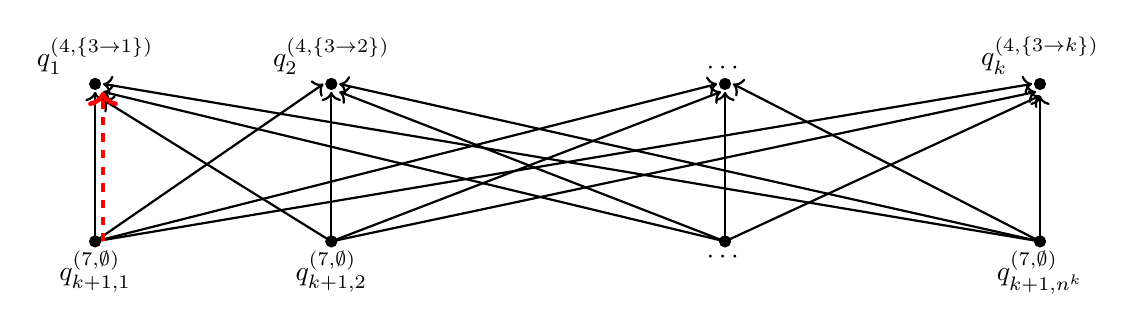
\begin{tikzpicture}
%%% The nodes represents the k query in the first round
\filldraw[black] (0, 2) circle (2pt) node [anchor=south]{$q_1^{(4, \{3 \to 1\} )}$};
\filldraw[black] (3, 2) circle (2pt) node [anchor=south]{$q_2^{(4, \{3 \to 2\} )}$};
% \filldraw[black] (6, 2) circle (2pt) node [anchor=south]{$q^4_3$};
\filldraw[black] (8, 2) circle (2pt) node [anchor=south]{$\cdots$};
\filldraw[black] (12, 2) circle (2pt) node [anchor=south]{$q_k^{(4, \{3 \to k\} )}$};
%%%%%% The nodes represents the n^k queries in the second round
\filldraw[black] (0, 0) circle (2pt) node [anchor=north]{$q_{k+1,1}^{(7, \emptyset)}$};
\filldraw[black] (3, 0) circle (2pt) node [anchor=north]{$q_{k+1,2}^{(7, \emptyset)}$};
% \filldraw[black] (6, 0) circle (2pt) node [anchor=north]{$q^{3, 7}_{k+1}$};
\filldraw[black] (8, 0) circle (2pt) node [anchor=north]{$\cdots$};
\filldraw[black] (12, 0) circle (2pt) node [anchor=north]{$q_{k+1,n^k}^{(7, \emptyset)}$};
%%%%%% The edges represents their dependency relations GROUP 1
\draw[ thick,->] (0, 0)  -- (0, 1.9) ;
\draw[ thick,->] (0, 0)  -- (2.9, 2) ;
% \draw[very thick,->] (0, 0)  -- (6, 2) ;
\draw[ thick,->] (0, 0)  -- (7.9, 2) ;
\draw[ thick,->] (0, 0)  -- (11.9, 2) ;
%%%%%% The edges represents their dependency relations GROUP 2
\draw[ thick,->] (3, 0)  -- (0.1, 1.8) ;
\draw[ thick,->] (3, 0)  -- (3, 1.9) ;
% \draw[very thick,->] (0, 0)  -- (6, 2) ;
\draw[ thick,->] (3, 0)  -- (7.95, 1.9) ;
\draw[ thick,->] (3, 0)  -- (11.95, 1.9) ;
%%%%%% The edges represents their dependency relations GROUP 3
\draw[ thick,->] (8, 0)  -- (0.1, 1.9) ;
\draw[ thick,->] (8, 0)  -- (3.1, 1.9) ;
% \draw[very thick,->] (0, 0)  -- (6, 2) ;
\draw[ thick,->] (8, 0)  -- (8, 1.9) ;
\draw[ thick,->] (8, 0)  -- (12, 1.85) ;
%%%%%% The edges represents their dependency relations GROUP 4
\draw[ thick,->] (12, 0)  -- (0.1, 2) ;
\draw[ thick,->] (12, 0)  -- (3.1, 2) ;
% \draw[very thick,->] (0, 0)  -- (6, 2) ;
\draw[ thick,->] (12, 0)  -- (8.1, 2) ;
\draw[ thick,->] (12, 0)  -- (12, 1.85) ;
%%%% The longest path representing the adaptivity
\draw[ultra thick, red, ->, dashed] (0.1, 0) -- (0.1, 1.9);
\end{tikzpicture}
}
\end{center}
\end{example}
%
\newpage

%
\begin{example}[Multi-Round Algorithm]
% \[
% MR^H \triangleq
% \begin{array}{l}
%     %  \left[j \leftarrow 0 \right]^1 ; \\
%     \left[I \leftarrow [] \right]^1; \\
%     \eloop ~ [k]^{2} ~  \\ 
%     \ ~ \edo ~ \\ \Big(
%     \left[p \leftarrow c \right]^3 ; \\
%     \left[a \leftarrow \query(p, I) \right]^4; \\
%     \left[I \leftarrow \eupdt( {I}, (a, p))  \right]^5
%     \Big) 
% \end{array}
% %
% ~~~~ \Rightarrow ~~~
% %
% MR^L \triangleq
% \begin{array}{l}
%     %  \left[j \leftarrow 0 \right]^1 ; \\
%     \left[I \leftarrow [] \right]^1; \\
%     \eloop ~ [k]^{2}  \\ 
%     \ ~ \edo ~ \\ \Big(
%     \left[p \leftarrow c \right]^3 ; \\
%     \left[
%     \eswitch \Big( I, a
%     \left(\begin{array}{l}
%         [ ] \to q_{j,1},\\
%         \cdots\\
%     \clabel{1, 2, 3, \cdots, n} \to q_{j,n!}
%     \end{array}\right)
%     \Big)
%     \right]^4;\\
%     \left[I \leftarrow \eupdt( {I}, (a, p))  \right]^5
%     \Big) 
% \end{array}
% \]
% Adapt($MR^L$) = 2 when $k=2$

% \[
% MR^{ssa} \triangleq
% \begin{array}{l}
%     %  \left[j \leftarrow 0 \right]^1 ; \\
%     \left[I_1 \leftarrow [] \right]^1; \\
%     \eloop ~ [k]^{2} , 0, [I_3,I_1,I_2] \\ 
%     \ ~ \edo ~ \\ \Big(
%     \left[p_1 \leftarrow c \right]^3 ; \\
%     \left[
%     \eswitch \Big( I_3, a_1
%     \left(\begin{array}{l}
%         [ ] \to q_{j,1},\\
%         \cdots\\
%     \clabel{1, 2, 3, \cdots, n} \to q_{j,n!}
%     \end{array}\right)
%     \Big)
%     \right]^4;\\
%     \left[I_2 \leftarrow \eupdt( {I_3}, (a_1, p_1))  \right]^5
%     \Big) 
% \end{array}
% \]
\jl{
\[
MR \triangleq
\begin{array}{l}
    \left[i \leftarrow 1 \right]^1 ; \\
    \left[I \leftarrow [] \right]^2; \\
   \ewhile ~ [i < k]^{3} 
    \ ~ \edo ~ \\ \Big(
    \left[p \leftarrow c \right]^4 ; \\
    \left[a \leftarrow \query(p, I) \right]^5; \\
    \left[I \leftarrow \eupdt( {I}, (a, p))  \right]^6 ; \\
    \left[i \leftarrow i + 1 \right]^7 \\
    \Big) 
\end{array}
%
~~~~ \Rightarrow ~~~
%
MR^{ssa} \triangleq
\begin{array}{l}
    \left[i \leftarrow 1 \right]^1 ; \\
   \left[I \leftarrow [] \right]^2; \\
   \ewhile ~ [i < k]^{3} 0, [I_3,I_1,I_2] \\ 
    \ ~ \edo ~ \\ \Big(
    \left[p_1 \leftarrow c \right]^4 ; \\
    \left[a \leftarrow \query(p_1, I_2) \right]^5; \\
    \left[I_2 \leftarrow \eupdt( {I_3}, (a_1, p_1))  \right]^6;\\
    \left[i \leftarrow i + 1 \right]^7 \\
    \Big) 
\end{array}
\]
}
%
%
% Let $k = 4$, given a specific database $D$, we have $\config{\emptyset, MR^L, [],\emptyset} \rightarrow \config{m, \eskip, t, w } $ and the trace as:
% %
% $$t = \left[(q^{4, \{2 \to 1\}}_{1, 1}, v_1), 
% (q^{4, \{2 \to 2\}}_{2, 3}, v_2),
% (q^{4, \{2 \to 3\}}_{3, 2}, v_3)
% (q^{4, \{2 \to 4\}}_{4, 3}, v_4)
% \right]$$
% \\
%
Adapt($MR$) = k.
\\
% Using \THESYSTEM, we first generate a global list $G$ from an empty list $[]$ and empty whlemap $\emptyset$.
%  \[[]; \emptyset; MR^{ssa} \to G; w  \land w = \emptyset\].
%  \[G_{k=2} = \left[
%   {I_1}^{(1,\emptyset)} , {I_3}^{(2,[2:1])} , {p_1}^{(3,[2:1])} , {a_1}^{(4,[2:1])} ,{I_2}^{(5,[2:1])} ,  {I_3}^{(2,[2:2])} , {p_1}^{(3,[2:2])} , {a_1}^{(4,[2:2])} ,{I_2}^{(5,[2:2])} , {I_3}^{(2,\emptyset)}   \right] \]
%   We denote $I_1^{1}$ short for ${I_1}^{(1,\emptyset)}$ and ${I_3}^{(2,1)}$ short for ${I_3}^{(2,[2:1])}$, where the label $(2, 1)$ represents at line number $2$ and in the $1$ st iteration. 
% \[
% M =  \left[ \begin{matrix}
%   I_1^{1} & I_3^{(2,1)} & p_1^{(3,1)} & a_1^{(4,1)} &I_2^{(5,1)}  & I_3^{(2,2)} & p_1^{(3,2)} & a_1^{(4,2)} & I_2^{(5,2)} & I_3^{2}\\
%   0 & 0 & 0 & 0 & 0 & 0 & 0 &0 &0&0  \\
%  1 & 0 & 0 & 0 & 0 & 0 & 0&0&0&0\\
%  0 & 0 & 0 & 0 & 0 & 0& 0& 0 &0&0\\
%  0 & 1 & 0 & 0 & 0 & 0 & 0& 0&0&0\\
%  0 & 1 & 1 & 1 & 0 & 0 & 0 & 0&0 &0\\
%  1 & 0 & 0 & 0 & 1 & 0 & 0& 0&0&0\\
%  0 & 0 & 0 & 0 & 0 & 0 & 0& 0&0&0\\
%  0 & 0 & 0 & 0 & 0 & 1 & 0& 0&0&0\\
%  0 & 0 & 0 & 0 & 0 & 1 & 1 & 1 &0 &0\\
% 1 & 0 & 0 & 0 & 0 & 0 & 0 & 0 &1&0 \\
%  \end{matrix} \right] 
% ~ , V = \left [ \begin{matrix}
% I_1^{1} &  0 \\
% I_3^{(2,1)} &  0 \\
% p_1^{(3,1)} & 0 \\
% a_1^{(4,1)} &  1 \\
% I_2^{(5,1)} & 0 \\
% I_3^{(2,2)} & 1 \\
% p_1^{(3,2)} &  0 \\
% a_1^{(4,2)} & 1 \\
% I_2^{(5,2)} & 0 \\
% I_3^{2} & 0 \\
% \end{matrix} \right ]
% \]
\jl{
Using \THESYSTEM, we first generate a global list $G$ from an empty list $[]$ and empty whlemap $\emptyset$.
 \[[]; \emptyset; MR^{ssa} \to G; w  \land w = \emptyset\].
 %
 \[
 G_{k=2} = 
 \left[
 i_1^{1}, I_1^2, i_3^3, I_3^3, p_1^4, a_1^5, I_2^6, i_2^7
\right] 
\]
  We denote $I_1^{1}$ short for ${I_1}^{(1,\emptyset)}$ and ${I_3}^{(2,1)}$ short for ${I_3}^{(2,[2:1])}$, where the label $(2, 1)$ represents at line number $2$ and in the $1$ st iteration.
  }
\jl{
	\[
M =  \left[ \begin{matrix}
   i_1^{1} & I_1^2 & i_3^3 & I_3^3 & p_1^4 & a_1^5 & I_2^6 & i_2^7\\
 0 & 0 & 0 & 0 & 0 & 0 & 0 & 0 \\
 1 & 0 & 0 & 0 & 0 & 0 & 0 & 0 \\
 0 & 0 & 0 & 0 & 0 & 0 & 0 & 0 \\
 0 & 1 & 0 & 0 & 0 & 0 & 0 & 0 \\
 0 & 1 & 1 & 1 & 0 & 0 & 0 & 0 \\
 1 & 0 & 0 & 0 & 1 & 0 & 0 & 0 \\
 0 & 0 & 0 & 0 & 0 & 0 & 0 & 0 \\
 0 & 0 & 0 & 0 & 0 & 1 & 0 & 0 \\
 0 & 0 & 0 & 0 & 0 & 1 & 1 & 1 \\
 1 & 0 & 0 & 0 & 0 & 0 & 0 & 0  \\
 \end{matrix} \right] 
~ , V = \left [ \begin{matrix}
i_1^1 & 0 \\
I_1^2 & 0 \\
i_3^3 & 2 \\
I_3^3 & 2 \\
p_1^4 & 2 \\
a_1^5 & 1 \\
I_2^6 & 2 \\
i_2^7 & 2
\end{matrix} \right ]
\]
}

\newpage
\begin{center}
%
\todo{
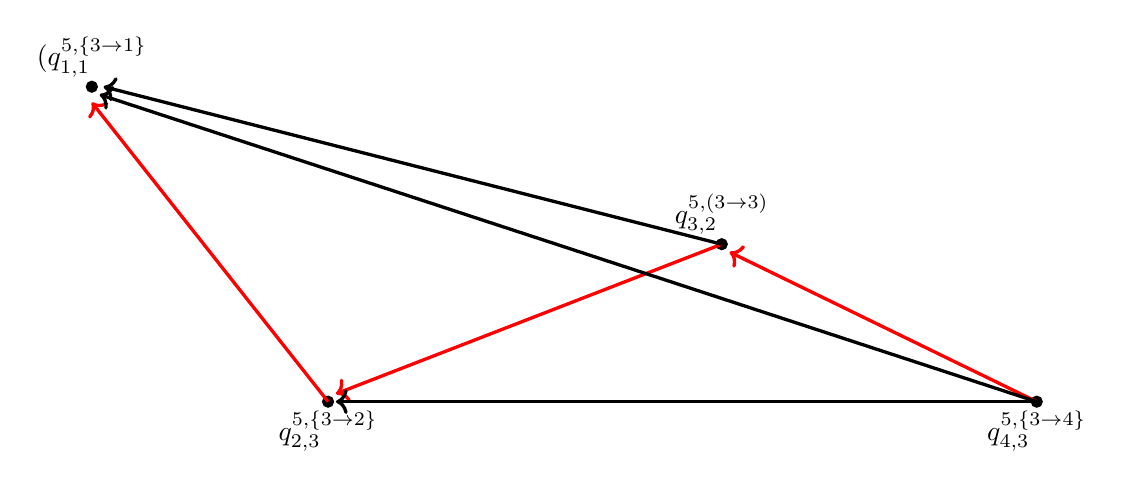
\begin{tikzpicture}
%%% The nodes represents the k query in the first round
\filldraw[black] (0, 4) circle (2pt) node [anchor=south]{$(q^{5, \{3 \to 1\}}_{1, 1}$};
% \filldraw[black] (8, 4) circle (2pt) node [anchor=south]{$\cdots$};
% \filldraw[black] (12, 4) circle (2pt) node [anchor=south]{$q^{1, (5, k)}_k$};
%%%%%% The nodes represents the n^k queries in the second round
% \filldraw[black] (0, 0) circle (2pt) node [anchor=north]{$q^{n!, (5, 1)}_1$};
\filldraw[black] (3, 0) circle (2pt) node [anchor=north]{$q^{5, \{3 \to 2\}}_{2, 3}$};
% \filldraw[black] (6, 0) circle (2pt) node [anchor=north]{$q^{3, 7}_{k+1}$};
% \filldraw[black] (8, 0) circle (2pt) node [anchor=north]{$\cdots$};
\filldraw[black] (12, 0) circle (2pt) node [anchor=north]{$q^{5, \{3 \to 4\}}_{4, 3}$};
%%% The nodes represents the k query in the first round
% \filldraw[black] (0, 2) circle (2pt) node [anchor=south]{$q^{\cdots, (5, 1)}_1$};
% \filldraw[black] (3, 2) circle (2pt) node [anchor=south]{$q^{\cdots, (5, 2)}_2$};
% \filldraw[black] (6, 2) circle (2pt) node [anchor=south]{$q^4_3$};
\filldraw[black] (8, 2) circle (2pt) node [anchor=south]{$q^{5, (3 \to 3)}_{3, 2}$};
% \filldraw[black] (12, 2) circle (2pt) node [anchor=south]{$q^{\cdots, (5, k)}_k$};
%%%%%% The edges represents their dependency relations GROUP 1
% \draw[very thick,->] (3, 2)  -- (0.1, 2) ;
% \draw[very thick,->] (3, 0)  -- (0.1, 1.9) ;
% \draw[very thick,->] (3, 4)  -- (0.1, 2.1) ;
% %
% \draw[very thick,->] (3, 2)  -- (0.1, 0.1) ;
% \draw[very thick,->] (3, 0)  -- (0.1, 0) ;
% \draw[very thick,->] (3, 4)  -- (0, 0.2) ;
% %
% \draw[very thick,->] (3, 2)  -- (0.1, 3.9) ;
\draw[very thick,->, red] (3, 0)  -- (0, 3.8) ;
% \draw[very thick,->] (3, 4)  -- (0, 4) ;
% \draw[very thick,->] (0, 0)  -- (6, 2) ;
%%%%%% The edges represents their dependency relations GROUP 2
% \draw[very thick,->] (0, 0)  -- (6, 2) ;
% \draw[very thick,->] (8, 2)  -- (3.1, 2) ;
% \draw[very thick,->] (8, 0)  -- (3.1, 1.9) ;
% \draw[very thick,->] (8, 4)  -- (3.1, 2.1) ;
%
\draw[very thick,->, red] (8, 2)  -- (3.1, 0.1) ;
\draw[very thick,->] (8, 2)  -- (0.15, 4) ;
% \draw[very thick,->] (8, 0)  -- (3.1, 0) ;
% \draw[very thick,->] (8, 4)  -- (3, 0.2) ;
% %
% \draw[very thick,->] (8, 2)  -- (3.1, 3.9) ;
% \draw[very thick,->] (8, 0)  -- (3, 3.8) ;
% \draw[very thick,->] (8, 4)  -- (3.1, 4) ;
%%%%%% The edges represents their dependency relations GROUP 4
% \draw[very thick,->] (0, 0)  -- (6, 2) ;
% \draw[very thick,->] (12, 2)  -- (8.1, 2) ;
\draw[very thick,->, red] (12, 0)  -- (8.1, 1.9) ;
\draw[very thick,->] (12, 0)  -- (3.1, 0) ;
\draw[very thick,->] (12, 0)  -- (0.1, 3.9) ;
% \draw[very thick,->] (12, 4)  -- (8.1, 2.1) ;
% %
% \draw[very thick,->] (12, 2)  -- (8.1, 0.1) ;
% \draw[very thick,->] (12, 0)  -- (8.1, 0) ;
% \draw[very thick,->] (12, 4)  -- (8, 0.2) ;
% %
% \draw[very thick,->] (12, 2)  -- (8.1, 3.9) ;
% \draw[very thick,->] (12, 0)  -- (8, 3.8) ;
% \draw[very thick,->] (12, 4)  -- (8.1, 4) ;
%
% \draw[very thick,->] (12, 2)  -- (8.1, 3.9) ;
%%%% The longest path representing the adaptivity
% \draw[ultra thick, red, ->, dashed] (3, 4.1)  -- (0.1, 4.1);
% \draw[ultra thick, red, ->, dashed] (8, 4.1)  -- (3.1, 4.1);
% \draw[ultra thick, red, ->, dashed] (12, 4.1)  -- (8.1, 4.1);
\end{tikzpicture}
}
\end{center}
%
\newpage
%
$\forall k. \forall D$, we have $A(TR^L) = (k - 1)$ given all possible execution traces.
\todo{
\begin{center}
%
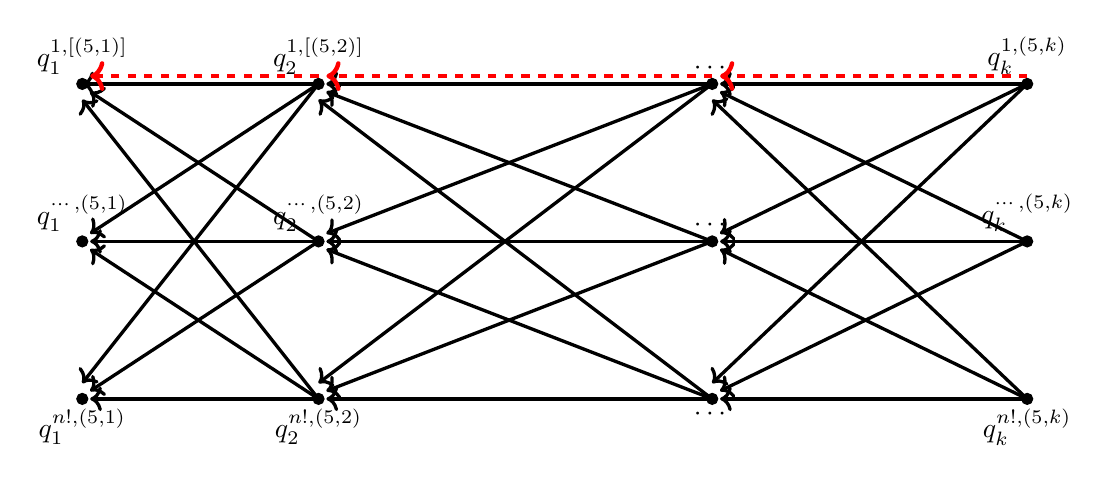
\begin{tikzpicture}
%%% The nodes represents the k query in the first round
\filldraw[black] (0, 4) circle (2pt) node [anchor=south]{$q^{1, [(5, 1)]}_1$};
\filldraw[black] (3, 4) circle (2pt) node [anchor=south]{$q^{1, [(5, 2)]}_2$};
% \filldraw[black] (6, 2) circle (2pt) node [anchor=south]{$q^4_3$};
\filldraw[black] (8, 4) circle (2pt) node [anchor=south]{$\cdots$};
\filldraw[black] (12, 4) circle (2pt) node [anchor=south]{$q^{1, (5, k)}_k$};
%%%%%% The nodes represents the n^k queries in the second round
\filldraw[black] (0, 0) circle (2pt) node [anchor=north]{$q^{n!, (5, 1)}_1$};
\filldraw[black] (3, 0) circle (2pt) node [anchor=north]{$q^{n!, (5, 2)}_2$};
% \filldraw[black] (6, 0) circle (2pt) node [anchor=north]{$q^{3, 7}_{k+1}$};
\filldraw[black] (8, 0) circle (2pt) node [anchor=north]{$\cdots$};
\filldraw[black] (12, 0) circle (2pt) node [anchor=north]{$q^{n!, (5, k)}_k$};
%%% The nodes represents the k query in the first round
\filldraw[black] (0, 2) circle (2pt) node [anchor=south]{$q^{\cdots, (5, 1)}_1$};
\filldraw[black] (3, 2) circle (2pt) node [anchor=south]{$q^{\cdots, (5, 2)}_2$};
% \filldraw[black] (6, 2) circle (2pt) node [anchor=south]{$q^4_3$};
\filldraw[black] (8, 2) circle (2pt) node [anchor=south]{$\cdots$};
\filldraw[black] (12, 2) circle (2pt) node [anchor=south]{$q^{\cdots, (5, k)}_k$};
%%%%%% The edges represents their dependency relations GROUP 1
\draw[very thick,->] (3, 2)  -- (0.1, 2) ;
\draw[very thick,->] (3, 0)  -- (0.1, 1.9) ;
\draw[very thick,->] (3, 4)  -- (0.1, 2.1) ;
%
\draw[very thick,->] (3, 2)  -- (0.1, 0.1) ;
\draw[very thick,->] (3, 0)  -- (0.1, 0) ;
\draw[very thick,->] (3, 4)  -- (0, 0.2) ;
%
\draw[very thick,->] (3, 2)  -- (0.1, 3.9) ;
\draw[very thick,->] (3, 0)  -- (0, 3.8) ;
\draw[very thick,->] (3, 4)  -- (0, 4) ;
% \draw[very thick,->] (0, 0)  -- (6, 2) ;
%%%%%% The edges represents their dependency relations GROUP 2
% \draw[very thick,->] (0, 0)  -- (6, 2) ;
\draw[very thick,->] (8, 2)  -- (3.1, 2) ;
\draw[very thick,->] (8, 0)  -- (3.1, 1.9) ;
\draw[very thick,->] (8, 4)  -- (3.1, 2.1) ;
%
\draw[very thick,->] (8, 2)  -- (3.1, 0.1) ;
\draw[very thick,->] (8, 0)  -- (3.1, 0) ;
\draw[very thick,->] (8, 4)  -- (3, 0.2) ;
%
\draw[very thick,->] (8, 2)  -- (3.1, 3.9) ;
\draw[very thick,->] (8, 0)  -- (3, 3.8) ;
\draw[very thick,->] (8, 4)  -- (3.1, 4) ;
%%%%%% The edges represents their dependency relations GROUP 4
% \draw[very thick,->] (0, 0)  -- (6, 2) ;
\draw[very thick,->] (12, 2)  -- (8.1, 2) ;
\draw[very thick,->] (12, 0)  -- (8.1, 1.9) ;
\draw[very thick,->] (12, 4)  -- (8.1, 2.1) ;
%
\draw[very thick,->] (12, 2)  -- (8.1, 0.1) ;
\draw[very thick,->] (12, 0)  -- (8.1, 0) ;
\draw[very thick,->] (12, 4)  -- (8, 0.2) ;
%
\draw[very thick,->] (12, 2)  -- (8.1, 3.9) ;
\draw[very thick,->] (12, 0)  -- (8, 3.8) ;
\draw[very thick,->] (12, 4)  -- (8.1, 4) ;
%
%%%% The longest path representing the adaptivity
\draw[ultra thick, red, ->, dashed] (3, 4.1)  -- (0.1, 4.1);
\draw[ultra thick, red, ->, dashed] (8, 4.1)  -- (3.1, 4.1);
\draw[ultra thick, red, ->, dashed] (12, 4.1)  -- (8.1, 4.1);
\end{tikzpicture}
\end{center}
}
\end{example}
%
%
% \begin{thm}
% [Observable Equivalent]
% Given a program $P$ in high level language, the corresponding low level language $P^l$ rewrote from $P$ via the rewriting rules is observably equivalent to $P$.
% \end{thm}
% %
% %
% \subsection{Adaptivity of the High Level Language}
% \begin{defn}
% [Adaptivity]
% Given a program $P$ in high level language, let $P^L$ be the set of all possible program in low level language observable equivalent to $P$, the adaptivity of $P$ is defined as:
% \\
% \[A(P) \triangleq \min\limits_{P^* \in P^L}A^*(P^*) \]
% %
% \end{defn}
% %
% %
% \subsection{Soundness of \THESYSTEM ~ in High Level Language}
% %
% \begin{thm}
% [Soundness]
% Given a program $P$ in high level language, let $P^l$ be the corresponding program in low level rewrote from $P$ via the rewriting rules, 
% then given $\Gamma$, $c_1$ and $c_2$ s.t. $\Gamma \subseteq FreeVar(P^l)$, 
% $ \Gamma \vdash^{c_1, c_2}_{M,V} P^l $, then we have:
% \\
% \[Adaptivity(P) \leq Adapt(M,V) \]
% \end{thm}
% %
% %
% %
% %
% \clearpage
% \section{Towards Probability}
% %
% \subsection{Syntax and Semantics}
% %
% \paragraph{Syntax.}
% \[
% \begin{array}{llll}
%  \mbox{Arithmetic Operators} & *_a & ::= & + ~|~ - ~|~ \times 
% %
% ~|~ \div \\  
%   \mbox{Boolean Operators} & *_b & ::= & \lor \sep \land \\
%   \mbox{Relational Operators} & *_r & ::= & < ~|~ \leq ~|~ = \\  
%  \mbox{Label} & l & & \\ 
%  \mbox{loop maps} & w & \in & \mbox{Label} \times \mathbb{N} \triangleq w +l \sep w \setminus l \sep w \oplus_\rho w \\
% \mbox{AExpr} & \aexpr & ::= & 
% ckk991``	%
% 	n ~|~ x ~|~ \aexpr *_a \aexpr ~|~ {[] ~|~ [\aexpr_0, \dots, \aexpr_i] \sep \aexpr \times \aexpr } \\
%     %
% \mbox{BExpr} & \bexpr & ::= & 
% 	%
% 	\etrue ~|~ \efalse  ~|~ \neg \bexpr
% 	 ~|~ \bexpr *_b \bexpr
% 	%
% 	~|~ \aexpr *_r \aexpr \\
% \mbox{Deterministic Expr} & \expr_d & ::=	& \aexpr \sep \bexpr \\
% \mbox{Randomized AExpr} & \aexpr_r & ::= & 
% 	%
% 	 x_r \sep n \sep  \aexpr_r *_a \aexpr_r \\
%     %
% \mbox{Randomized BExpr} & \bexpr_r & ::= & 
% 	%
% \neg \bexpr_r
% 	 ~|~ \bexpr_r *_b \bexpr_r
% 	%
% 	~|~ \aexpr_r *_r \aexpr_r \\
% \mbox{Randomized Expr} & \expr_r & ::=	& \expr_d \sep \aexpr_r \sep \bexpr_r \\
% \mbox{Command} & \command & ::= &   [\assign x {\expr_d}]^{l} \sep [\assign {x_r} {\expr_r}]^{l} \sep  [\assign x q]^{l} \sep  [\assign {x_r} \uniform ]^{l} \sep   [\assign {x_r} \bernoulli]^{l} 
%  %
% \\
% 	%
% & & & ~|~  \command ; \command  ~|~ \eif_D ([\bexpr]^{l}, \command_1, \command_2) \sep  \eif_R ([\bexpr_r]^{l}, \command_1, \command_2) 
%  ~|~ [\eskip]^{l} \\
% & & & { \sep [\eswitch( \expr, x, (v_i \to  q_i))]^{l}} \sep {\eloop ~ [\valr_N]^{l} ~ (f) ~ \edo ~ \command }
% 	\\
% 	%
% % \mbox{Binary Operation} & \bop & ::= & + ~|~ - ~|~ \times 
% % %
% \mbox{Memory} & m & ::= & [] ~|~ m[x^{l} \to v] \\
% %
% \mbox{Trace} & t & ::= & [] ~|~ [(q, v)^{(l, w) }] ~|~ t ++ t 
% ~|~ t \oplus_{\rho} t
% \end{array}
% \]
% %
% \[
% \begin{array}{ccl}
% w \setminus l     & = &\left \{  
%     \begin{array}{lr} w  & l \not\in Keys(w)   \\
%       w_l & Otherwise \\
%      \end{array} \right.\\
% w + l & = &
%  \left \{  
%     \begin{array}{lr}
%     w[l \to 0] & l \not \in Keys(w) \\   
%     w_l [l \to w(l)+1] & Otherwise
%           \end{array} \right.\\
% \end{array}
% \]
% %
% %
% %
\section{Analysis of Generalization Error}

\begin{example}[Two Round Algorithm]
\[
TR^H(k) \triangleq
{
\begin{array}{l}
    % \left[j \leftarrow 0 \right]^1 ; \\
    \clabel{a_1 \leftarrow [] }^1; \\
    \eloop ~ [k]^{2} ~ (a_2 \leftarrow f(1, a_1, a_3)) \\
    ~ \edo ~ \\
    \Big(
     \clabel{x_1 \leftarrow \query() }^3 ; \\
    \clabel{a_3 \leftarrow x_1 :: a_2 }^4     \Big);\\
    \clabel{l \leftarrow q_{k + 1}(a_3)}^{5}\\
\end{array}
}
\]
\end{example}
%
\begin{example}[Multi-Round Algorithm]
\[
MR^H \triangleq
\begin{array}{l}
    %  \left[j \leftarrow 0 \right]^1 ; \\
    \left[I_2 \leftarrow [] \right]^1; \\
    \eloop ~ [k]^{2} ~ (I_2 \leftarrow f(2, I_1, I_3)) \\ 
    \ ~ \edo ~ \\ \Big(
    \left[p_1 \leftarrow c \right]^3 ; \\
    \left[a_1 \leftarrow \delta(\query(p, I_2)) \right]^4; \\
    \left[I_3 \leftarrow \eupdt( {I_2}, (a_1, p))  \right]^5
    \Big) 
\end{array}
\]
\end{example}
%
%
By applying different mechanisms $\delta()$ over the queries $\query(\cdot)$, we have different error bounds.
\\
\textbf{Gaussian Mechanism:} $N(0, \sigma)$ \cite{dwork2015preserving}:
\\
Adaptivity $r = 2$: 
$ \sigma = O \left(\frac{\sqrt{r \log(k)}}{\sqrt{n}} \right)$ (also known as expected error);
\\
Adaptivity unknown:
$ \sigma = O\left(\frac{\sqrt[4]{k}}{\sqrt{n}} \right)$;
\\
{Mean Squared Error Bound:} 
$ \frac{1}{2n} \min\limits_{\lambda \in [0, 1]}
\left( \frac{2\rho k n - \ln(1 - \lambda)}{\lambda} 
\right)
+ 2 \mathbb{E}_{Z_i \sim N(0, \frac{1}{2n^2 \rho})}
\left[ \max\limits_{i \in [k]} (Z_i^2) \right]$
%
\\
{Confidence Bounds:} minimize $\tau$ where
$\tau \geq \sqrt{\frac{2}{n \beta}
\min\limits_{\lambda \in [0, 1]}
\left( \frac{2\rho k n - \ln(1 - \lambda)}{\lambda} 
\right)
}$
and 
$\tau \geq \frac{2}{n} \sqrt{\frac{\ln(4n /\beta}{\rho'}}$ with confidence level $1 - \beta$ .
\\
\textbf{$(\epsilon, \delta)-DP$ mechanism}:
\\
Confidence Bounds:
$\tau \geq \sqrt{\frac{48}{n} \ln(4/\beta) }$ with $\epsilon \leq \frac{\tau}{4}$ and $\delta = 
\exp \left(\frac{-4 \ln (8/\beta)}{\tau} \right)$
\\
\textbf{Sample Splitting}: 
\\
Expected Error: $O \left(\frac{\sqrt{k \log(k)}}{\sqrt{n}} \right)$
\\
\textbf{Thresholdout}: $B, \sigma, T, h$ 
\\
Confidence bounds:  
$\tau = \max\limits\left\{ 
\sqrt{\frac{2\zeta }{h \beta}},
2\sigma \ln(\frac{\beta}{2}),
\sqrt{\frac{1}{\beta}} \cdot \left(\sqrt{T^2 + 56\sigma^2} + \sqrt{\frac{\zeta}{4h} } \right)
\right\}
$,
for $\zeta = \min\limits_{\lambda \in [0, 1)}
\left( \frac{2B \ (\sigma^2 h) - \ln(1 - \lambda)}{\lambda} \right)$


% \begin{mathpar}
% \inferrule
% {M = \mathsf{L}(i) * ( \mathsf{R}(\expr,i) + \Gamma )
% }
% {\Gamma \vdash_{M, V_{\emptyset}}^{(i, i+1)} \assign {x}{\expr} 
% }
% ~\textbf{asgn}
% \and
% \inferrule
% {M = \mathsf{L}(i) * ( \Gamma)
% \\
% V= \mathsf{L}(i)
% }
% { \Gamma \vdash^{(i, i+1)}_{M, V} \assign{x}{q} : 
% }~\textbf{query}
% %
% \and 
% %
% \inferrule
% {
% \Gamma + \mathsf{R}(\bexpr) \vdash^{(i_1, i_2)}_{M, V} c_1 
% : \Phi \land \bexpr \Rightarrow \Psi
% \and 
% \Gamma + \mathsf{R}(\bexpr) \vdash^{(i_2, i_3)}_{M, V} c_2 
% : \Phi \land \neg \bexpr \Rightarrow \Psi
% }
% {
% \Gamma \vdash^{(i_1, i_3)}_{M, V} 
% \eif ~ \bexpr \ethen c_1 \eelse c_2 : \Phi \Rightarrow \Psi
% }~\textbf{if}
% %
% %
% %
% \and 
% %
% \inferrule
% {
% \Gamma \vdash^{(i_1, i_2)}_{M_1, V_1} c_1 : \Phi \Rightarrow \Phi_1
% \and 
% \Gamma \vdash^{(i_2, i_3)}_{M_2, V_2} c_2 : \Phi_1 \Rightarrow \Psi 
% }
% {
% \Gamma \vdash^{(i_1, i_3)}_{M_1 ; M_2, V_1 \uplus V_2}
% c_1 ; c_2 : \Phi \Rightarrow \Psi
% }
% ~\textbf{seq}
% \and 
% \inferrule
% {
% \forall 0 \leq z < N. 
% {\Gamma \vdash^{(i,i+a )}_{M_1, V_1} c_1 : \Phi \land e_n = \lceil{z+1}\rceil \Rightarrow \Psi }
% \and
% {\Gamma \vdash^{(i+a,i+b )}_{M, V} c_2 : \Psi \Rightarrow \Phi \land e_N = \lceil{z}\rceil }
% \and
% { e_N = \lceil {N} \rceil }
% }
% {\Gamma \vdash^{(i, i+ N*b)}_{M_{i,b}^N(c_1), V_{i, b}^N} 
% \eloop ~ \expr_N ~ (c_1) ~ \edo ~ c_2 : \Phi \land \expr_N = \lceil { N} \rceil \Rightarrow \Phi \land \expr_N = \lceil{0}\rceil
% }~\textbf{loop}
% % \and 
% % \inferrule
% % {
% % \Gamma \vdash^{(i,i+a )}_{M, V} c 
% % }
% % {\Gamma \vdash^{(i, i+ N*a)}_{M_{i,a}^N(f), V_{i, a}^N} 
% % \ewhile([\bexpr]^l,   c) : \phi \Rightarrow \psi
% % }~\textbf{while}
% %
% \and
% %
% \inferrule
% { \Gamma + \mathsf{R}(\expr) \vdash^{(i_1+j-1, i_1+j)}_{M_j, V_j} \assign{ x_j}{q_j} : \Phi \Rightarrow \Psi
% \\
% j \in \{1, \dots, N\}     }
% {\Gamma \vdash^{(i_1, i_1+N)}_{ \sum_{j=0}^{N} M_j, \sum_{j=0}^{N} V_j} \eswitch(\expr, x,(v_j \rightarrow q_j ) : \Phi \Rightarrow \Psi }
% ~\textbf{switch}
% %
% \and
% %
% \inferrule
% { 
% \vDash 
% \Phi \Rightarrow \Phi'  
% \and
% \Gamma \vdash^{(i_1, i_2)}_{(M',V')} c : \Phi' \Rightarrow \Psi'
% \and
% \vDash \Psi' \Rightarrow \Psi
% \and 
% \Phi \vDash M' \leq M
% \and 
% \Phi \vDash V' \leq V
% }
% {\Gamma \vdash^{(i_1, i_2)}_{(M,V)} c 
% : \Phi \Rightarrow \Psi
% }
% ~\textbf{conseq}
% \end{mathpar}

\clearpage

\section{new \THESYSTEM with loop }
\subsection{Analysis Rules/Algorithms of \THESYSTEM}

There are two steps for our algorithm to get the estimation of the adaptivity of a program $\ssa{c}$ in the ssa form. 
\begin{enumerate}
    \item Estimate the variables that are new generated (via assignment) and store these variables in a global list $G$. We have the algorithm of the form : $\ag{ G;w; \ssa{c}}{G';w'} $.
    \item We start to track the dependence between variables in a matrix $M$, whose size is $|G| \times |G|$, and track whether arbitrary variable is assigned with a query result in a vector $V$ with size $|G|$. The algorithm to fill in the matrix is of the form: $\ad{\Gamma ; \ssa{c} ; i_1}{M;V;{i_2}}$. $\Gamma$ is a vector records the variables the current program $\ssa{c}$ depends on, the index $i_1$ is a pointer which refers to the position of the first new-generated variable in $\ssa{c}$ in the global list $G$, and $i_2$ points to the first new variable that is not in $\ssa{c}$ (if exists). 
\end{enumerate}

% We have the judgment of the form $\vdash^{i_1, i_2}_{M,V} ~ c  $.  Our grade is a combination of a matrix $M$, used to track the dependency of variables appeared in the statement $c$, and a vector $V$ indicating the variables associated with results from queries $q$. The size of the matrix $M$ is $L \times L$, and vector $V$ of size $L$, where $L$ is the total size of variables needed in the program $c$, which is fixed per program. We assume the program is in the style of Static Single Assignment.To be more specific, we give a quick example: $x \leftarrow e_1; x \leftarrow e_2 $ will be rewritten as $ x_1 \leftarrow e_1; x_2 \leftarrow e_2$. And the if condition $ \eif ~ e_b \ethen x \leftarrow e_1 \eelse x \leftarrow e_2  $ will look like $ \eif ~ e_b \ethen x_1 \leftarrow e_1 \eelse x_2 \leftarrow e_2  $. As we have seen, SSA requires unique variables, and these newly generated variables will be recorded in the matrix $M$.  Also, the variable at different iteration is treated as different variable in the matrix $M$ and vector $V$.

% The superscript $i_1,i_2$  specify the range of "living" or "active" variables in the matrix and vector. $i_1$ is the starting line (and column) in the matrix where the new generated variables in program $c$ starts to show up. Likewise, $i_2$ states the ending position of active range by $c$.
%  Worth to mention, $i_1,i_2$ can be used to track the exact location of newly generated variables. For example, the assignment statement $x \leftarrow e$ or $x \leftarrow q $ with $c_2 =c_1+1$, tells us the variable $x$ is at the $c_1$th line(column) of the matrix. As we can notice, the loop increases the variables needed in the matrix by $N \times a$ where $N$ is the number of rounds of the loop and $a$ is the size of the variables generated in the loop body. We will have a global map, which maps the variable name to the position in the vector. We call it $GM: VAR \to \mathbb{N}$.

We give an example of $M$ and $V$ of the program $c$.   
$$
c= \begin{array}{c}
\ssa{\assign {x_1} {q}} ;        \\
\ssa{\assign {x_2} {x_1+1}} ;\\
\ssa{\assign {x_3} {x_2+2} }
\end{array}~~~~~~~~~~~~
M =  \left[ \begin{matrix}
 & (x_1) & (x_2) & (x_3) \\
(x_1) & 0 & 0 & 0 \\
(x_2) & 1 & 0 & 0 \\
(x_3) & 1 & 1 & 0 \\
\end{matrix} \right] ~ , V = \left [ \begin{matrix}
(x_1) &  1 \\
(x_2) & 0 \\
(x_3) & 0 \\
\end{matrix} \right ]
$$
Still use the program $c$ as the example, the global list $G$ is now : $ [ x_1 , x_2 , x_3] $. 
The function $\mathsf{Left}$ and $\mathsf{Right}$ is used to generate the corresponding vector of the left side and right side of an assignment. Take $\assign {x_2} {x_1+1} $ as an example, the result is shown as follows.
\[
\sf{L}(1) = \left[ \begin{matrix}
 0  & ~~~(x_1) \\
 1 & ~~~(x_2) \\
 0 & ~~~(x_3) \\
\end{matrix}   \right ] ~~~~~~~~~~~~~~
\sf{R} (x_1+1, 1) = \left[ \begin{matrix} 
   1 & 0 & 0 \\
   (x_1) & (x_2) & (x_3) \\
\end{matrix}  \right]
\]
Now let us think about the loop.
\[\ssa{c_3} \triangleq
\begin{array}{l}
     \left[\ssa{ x_1 \leftarrow q_1}  \right]^1 ; \\
    \eloop ~ [2]^{2} , 0,\\
  \ssa{[x_3 , x_1 , x_2]} 
     ~ \edo
    \\
    ~ \Big( 
    \left[\ssa{ y_1 \leftarrow q_2} \right]^3; \\
    \left[\ssa{x_2 \leftarrow y_1  + x_3 } \right]^5
    \Big) ; \\
     \left[ \assign{z_1}{x_3 + 2}  \right]^{6}
\end{array}
~~~~~~~~~~~~
M =  \left[ \begin{matrix}
 & (x_1) & (x_3^{1}) & (y_1^{1}) & (x_3^{1})  & (x_3^{2}) & (y_1^{2}) & (x_2^{2}) & (x_3^{f}) &  (z_1) \\
(x_1) & 0 & 0 & 0 & 0 & 0 & 0 & 0 &0 &0 \\
(x_3^{1}) & 1 & 0 & 0 & 0 & 0 & 0 & 0&0&0\\
(y_1^{1}) & 0 & 0 & 0 & 0 & 0 & 0& 0& 0 &0\\
(x_2^{1}) & 0 & 1 & 1 & 0 & 0 & 0 & 0& 0&0\\
(x_3^{2}) & 0 & 0 & 0 & 1 & 0 & 0 & 0 & 0&0 \\
(y_1^{2}) & 0 & 0 & 0 & 0 & 0 & 0 & 0& 0&0\\
(x_2^{2}) & 0 & 0 & 0 & 0 & 1 & 1 & 0& 0&0\\
(x_3^{f}) & 1 & 0 & 0 & 0 & 0 & 0 & 1& 0&0\\
(z_1) & 0 & 0 & 0 & 0 & 0 & 0 & 0 & 1 &0 \\
\end{matrix} \right] ~ , V = \left [ \begin{matrix}
(x_1) &  1 \\
(x_3^{1}) & 0 \\
(y_1^{1}) & 1 \\
(x_2^{1}) &  0 \\
(x_3^{2}) & 0 \\
(y_1^{2}) & 1 \\
(x_2^{2}) &  0 \\
(x_3^{f}) &  0 \\
(z_1) &  0 \\
\end{matrix} \right ]
\]

\[\ssa{c_3'} \triangleq
\begin{array}{l}
     \left[\ssa{ x_1 \leftarrow q_1}  \right]^1 ; \\
    \eloop ~ [0]^{2} , 0,\\
  \ssa{[x_3 , x_1 , x_2]} 
     ~ \edo
    \\
    ~ \Big( 
    \left[\ssa{ y_1 \leftarrow q_2} \right]^3; \\
    \left[\ssa{x_2 \leftarrow y_1  + x_3 } \right]^5
    \Big) ; \\
    \left[ \assign{z_1}{x_3 + 2}  \right]^{6}
\end{array}
~~~~~~~~~~~~
M =  \left[ \begin{matrix}
 & (x_1) & (x_3^{f}) & (z_1)  \\
(x_1) & 0 & 0 & 0 \\
(x_3^{f}) & 1 & 0 & 0 \\
(z_1^{2}) & 0 & 1 & 0 \\
\end{matrix} \right] ~ , V = \left [ \begin{matrix}
(x_1) &  1 \\
(x_3^{f}) & 0 \\
(z_1) &  0 \\
\end{matrix} \right ]
\]
We can now look at the if statement.
\[ c_4 \triangleq
\begin{array}{l}
   \left[ x \leftarrow q_1 \right]^1; \\
   \left[y \leftarrow q_2\right]^2 ; \\
    \eif \;( x + y == 5 )^3\; \\
    \mathsf{then} \;\left[ x \leftarrow q_3 \right]^4 \; \\
    \mathsf{else} (\;\left[ x \leftarrow q_4 \right]^5 ; \\
    y \leftarrow 2 ) ;\\
   \left[ z \leftarrow x +y \right]^6; \\
\end{array}
\hspace{20pt} \hookrightarrow \hspace{20pt}
%
 \ssa{c_4} \triangleq
\begin{array}{l}
   \left[ \ssa{ x_1 \leftarrow q_1} \right]^1; \\
   \left[\ssa{ y_1 \leftarrow q_2} \right]^2 ; \\
    \eif \;( \ssa{ x_1 + y_1 == 5} )^3, [ x_4,x_2,x_3 ],[] ,[y_3,y_1,y_2 ]\; \\
    \mathsf{then} \;\left[ \ssa{ x_2 \leftarrow q_3}\right]^4 \; \\
    \mathsf{else} (\;\left[ \ssa{x_3 \leftarrow q_4} \right]^5 ; \\
     \ssa{y_2 \leftarrow 2} ) \\
   \left[ \ssa{ z_1 \leftarrow x_4 +y_3 }\right]^6; \\
\end{array}
\]
\[
M_{c4} =  \left[ \begin{matrix}
 & (x_1) & (y_1) & (x_2) & (x_3)  & (y_2) & (x_4) & (y_3) & (z_1)  \\
(x_1) & 0 & 0 & 0 & 0 & 0 & 0 & 0 &0  \\
(y_1) & 0 & 0 & 0 & 0 & 0 & 0 & 0&0\\
(x_2) & 0 & 0 & 0 & 0 & 0 & 0& 0& 0 \\
(x_3) & 0 & 0 & 0 & 0 & 0 & 0 & 0& 0\\
(y_2) & 0 & 0 & 0 & 0 & 0 & 0 & 0 & 0 \\
(x_4) & 0 & 0 & 1 & 1 & 0 & 0 & 0 &0\\
(y_3) & 0 & 1 & 0 & 0 & 1 & 0 & 0 &0\\
(z_1) & 0 & 0 & 0 & 0 & 0 & 1 & 1 & 0  \\
\end{matrix} \right] ~ , V_{c4} = \left [ \begin{matrix}
(x_1) &  1 \\
(y_1) & 1 \\
(x_2) & 1 \\
(x_3) &  1 \\
(y_2) & 0 \\
(x_4) & 0 \\
(y_3) &  0 \\
(z_1) &  0 \\
\end{matrix} \right ]
\]
% We consider to have the superscript to denote the iteration number (or map if we have nested loop), as shown in the above matrix and vector. The global map $G$ is generated by analysing the program. We can estimate the variables needed in the loop by using the loop number $N$ and the loop body. In this example, the global map for $c_3$ : $ \{ x_1 \to 1, x_2^{1} \to 2, y_1^{1} \to 3 , x_3^{1} \to 4 , x_2^{2} \to 5 , y_1^{2} \to 6 , x_3^{2} \to 7  \} $.  
% By default, $G(x_2)$ gives the location for the first appearance of the variable $x_2$. We can also allow $G(x_2 , 2)$ to get the location of the second iteration $x_2^{2}$. We also allow $G(x, i, i+n)$ to return a set of locations where $x$ appears in the vector in the certain range $[i, i+n]$, which helps to locate variables in the loop.




% Also, to be able to track the relation between variables in varied iterations in the loop. we define a dependent map $\mathsf{DM}$ based on command $c$ to provide the dependency relation(syntactically) between variables. $\mathsf{VAR}(\expr)$ gives the set of variables appears in the expression $\expr$.
% \[
% \begin{array}{lll}
% \mathsf{DM} (c_1; c_2) & \triangleq &  \mathsf{DM} (c_1) \uplus \mathsf{DM} (c_2)  \\
% \mathsf{DM} (x_1 \leftarrow \expr ) & \triangleq & \{  x_1 \to \mathsf{VARS}(\expr)  \}
% \end{array}
% \]

\subsection{The algorithm to estimate the matrix and vector}
We first generate a list of variables $G$ that will be assigned with values (via the command $\assign{x}{e}$ or $\assign{x}{q}$). 

 \begin{mathpar}
\inferrule
{
}
{ \ag{G ;w; \ssa{[\assign {x}{\expr}]^{l}}}{G ++ [\ssa{x}^{(l,w)}];w}
% G ;w; \ssa{[\assign {x}{\expr}]^{l}} \to G ++ [x^{(l,w)}];w 
}
~\textbf{ag-asgn}
\and
\inferrule
{
}
{ \ag{G ;w;  [ \assign{\ssa{x}}{q(\ssa{\expr})}]^{l}}{  G ++ [\ssa{x}^{(l,w)}] ; w} 
}~\textbf{ag-query}
%
\and 
%
\inferrule
{
\ag{G; w; \ssa{c_1}}{  G_1;w_1}
\and 
 \ag{G_1;w ; \ssa{c_2}}{  G_2; w_2}
 \\
 {G_3 = G_2 ++ \ssa{[\bar{x}^{(l,w)}]++ \ssa{[\bar{y}^{(l,w)}]}++ \ssa{[\bar{z}^{(l,w)}]} }}
}
{
\ag{G; w;
[\eif(\ssa{\bexpr},[ \bar{\ssa{x}}, \bar{\ssa{x_1}}, \bar{\ssa{x_2}}] ,[ \bar{\ssa{y}}, \bar{\ssa{y_1}}, \bar{\ssa{y_2}}],[ \bar{\ssa{z}}, \bar{\ssa{z_1}}, \bar{\ssa{z_2}}], \ssa{ c_1, c_2)}]^{l} }{ G_3 ;w}
}~\textbf{ag-if}
%
%
%
\and 
%
\inferrule
{
\ag{G; w; \ssa{c_1}}{ G_1; w_1}
\and 
\ag{G_1;w_1; \ssa{c_2}}{ G_2; w_2}
}
{
\ag{G; w;
\ssa{(c_1 ; c_2)}}{  G_2 ; w_2}
}
~\textbf{ag-seq}
\and 
\inferrule
{
{G_0 = G \quad w_0 =w }
\and
\forall 0 \leq z < N. 
{ \ag{ G_z ++ \ssa{[\bar{x}^{(l, {w_z}+l)}]} ; (w_z+l); \ssa{c}}{ G_{z+1} ; w_{z+1}}  }
\\
{G_f = G_N ++ \ssa{[\bar{x}^{(l, w_N \setminus l)}]} }
\and
{ \ssa{\aexpr} =  {N}  }
}
{\ag{G; w; [\eloop ~ \ssa{\aexpr}, n, [\bar{\ssa{x}}, \bar{\ssa{x_1}}, \bar{\ssa{x_2}}] ~ \edo ~ \ssa{c}]^{l} }{ G_f; w_N\setminus l }
}~\textbf{ag-loop}
\end{mathpar}


%
%
% \paragraph{Analysis Rules.}
% \[\begin{array}{ll}
%     \mathcal{A}( \assign x \expr )( \Gamma , i )  & =  ( \mathsf{L}(x) * ( \mathsf{R}(\expr) + \Gamma ), V, i+1 )\\
%     \mathcal{A}( \assign x q)( \Gamma ,  i )  & = ( \mathsf{L}(x) * ( \mathsf{R}(\emptyset) + \Gamma) , \mathsf{L}(x) , i+1 )\\
%     \mathcal{A}( \eif ~ e_b \ethen c_1 \eelse c_2 )( \Gamma , i ) & =   \elet \; (M_1, v_1, i_1) =  \mathcal{A}(C_1)(\Gamma +\mathsf{R}(e_b) , i)
%     \ein \; \\
%     &  \elet \;  (M_2, v_2, i_2)= \mathcal{A}(C_2) (\Gamma +\mathsf{R}(e_b) ,i_1) \ein \; \\
%     & (  M_1 \uplus M_2, V_1 \uplus V_2   , i_2 )
%     \\
%     \mathcal{A}( c_1 ; c_2 )( \Gamma ,  i )  & =  \elet \;     (M_1, v_1, i_1) = 
%     \mathcal{A}(c_1) (\Gamma  +\mathsf{R}(e_b) , i)
%     \ein \; \\
%     &  \elet \;  (M_2, v_2, i_2) =                      \mathcal{A}(c_2)(\Gamma +\mathsf{R}(e_b) ,
%       i_1) \ein \; \\ 
%       & (  M_1 \cdot M_2, V_1 \uplus V_2   , i_2 )    \\
%      \mathcal{A}( \eloop ~ \expr_N ~ (c_1) ~ \edo ~ c_2  )( \Gamma ,  i )  & =  \elet \;     (M_1, v_1, i+a) = 
%     \mathcal{A}(c_1;c_2 ) (\Gamma , i)
%     \ein \; \\
%     & ( M_{i,a}^N(c_1), V_{i, a}^N , i + N*a ) \\
%  \mathcal{A}( \eswitch(\expr, x,(v_j \rightarrow q_j )  )( \Gamma ,  i+j )  & =  \elet \;     (M_j, v_j, i+j) = 
%     \mathcal{A}(x_j \leftarrow q_j ) (\Gamma + \mathsf{R}(e), i+j-1)     
%   \ein \\
%   & ( \sum_{j=0}^{N} M_j, \sum_{j=0}^{N} V_j, i + N ) \quad j \in \{1, \dots, N\}  \\
%     \end{array}
% \]
%
%
\paragraph{Analysis Logic Rules.}
%
%
$\Gamma$ is a matrix of one row and $N$ columns, $N = |G|=|V|$.\\ 

$\mathsf{L(i)}$ generates a matrix of one column, $N$ rows, where the $i-th$ row is $1$, all the other rows are $0$.\\

$\mathsf{R(e, i)}$ generates a matrix of one row and $N$ columns, where the locations of variables in $e$ is marked as $1$. To handle loop, for instance, the variable $y$ appears many times in $G$, the argument $i$ helps to find the location of the current living variable $y$ in the expression $e$, which is the latest $y$ with the largest location $i_y< i$ in our global variable list $G$.\\ 


{$ \forall 0 \leq z < |\bar{x}|. \bar{x}(z) = x_z, \bar{x_1}(z) = x_{1z}, \bar{x_2}(z) = x_{2z} $ } \\

$ \Gamma \vdash_{M,v_{\emptyset}}^{i, i+ |\ssa{\bar{x}}|} \ssa{[ \bar{x},\bar{x_1},\bar{x_2}   ]} \triangleq { \forall 0 \leq z < |\bar{x}|.  \Gamma \vdash_{M_{x_z}, V_{\emptyset}}^{i+z, i+z+1 } x_z \leftarrow x_{1z} + x_{2z} }$ where $M = \sum_{z\in [|\bar{x}|] }M_{x_z} $\\

\framebox{$ {\Gamma} \vdash^{i_1, i_2}_{M,V} ~ c $}
%
% \begin{mathpar}
% \inferrule
% {M = \mathsf{L}(i) * ( \mathsf{R}(\expr,i) + \Gamma )
% }
% {\Gamma \vdash_{M, V_{\emptyset}}^{(i, i+1)} [\assign {\ssa{x}}{\ssa{\expr}} ]^{l}
% }
% ~\textbf{asgn}
% \and
% \inferrule
% {M = \mathsf{L}(i) * ( \Gamma)
% \\
% V= \mathsf{L}(i)
% }
% { \Gamma \vdash^{(i, i+1)}_{M, V} [ \assign{\ssa{x}}{q} ]^{l} 
% }~\textbf{query}
% %
% \and 
% %
% \inferrule
% {
% \Gamma + \mathsf{R}(\bexpr, i_1) \vdash^{(i_1, i_2)}_{M_1, V_1} \ssa{c_1} 
% % : \Phi \land \bexpr \Rightarrow \Psi
% \and 
% \Gamma + \mathsf{R}(\bexpr, i_1) \vdash^{(i_2, i_3)}_{M_2, V_2} \ssa{c_2} 
% % : \Phi \land \neg \bexpr \Rightarrow \Psi
% \\
% { \forall 0 \leq j < |\bar{x}|. \bar{x}(j) = x_j, \bar{x_1}(j) = x_{1j}, \bar{x_2}(j) = x_{2j}  }
% \\
% { \forall 0 \leq j < |\bar{x}|.  \Gamma \vdash_{M_{x_j}, V_{\emptyset}}^{i_3+j, i_3+j+1 } x_j \leftarrow x_{1j} + x_{2j} }
% \and
% { \forall 0 \leq j < |\bar{y}|.  \Gamma \vdash_{M_{y_j}, V_{\emptyset}}^{i_3+|\bar{x}|+j, i_3+|\bar{x}|+j+1 } y_j \leftarrow y_{1j} + y_{2j} }
% \\
% { \forall 0 \leq j < |\bar{z}|.  \Gamma \vdash_{M_{z_j}, V_{\emptyset}}^{i_3+|\bar{x}|+|\bar{y}|+j, i_3+|\bar{x}|+|\bar{y}|+j+1 } z_j \leftarrow z_{1j} + z_{2j} }
% \and
% {M = (M_1+M_2)+ \sum_{j\in [|\bar{x}|] }M_{x_j} + \sum_{j\in [|\bar{y}|] }M_{y_j} + \sum_{j\in [|\bar{z}|] }M_{z_j} }
% }
% {
% \Gamma \vdash^{(i_1, i_3+|\bar{x}|+|\bar{y}|+|\bar{z}|)}_{M, V_1 \uplus V_2 } 
% [\eif(\sbexpr,[ \bar{\ssa{x}}, \bar{\ssa{x_1}}, \bar{\ssa{x_2}}] ,[ \bar{\ssa{y}}, \bar{\ssa{y_1}}, \bar{\ssa{y_2}}] , [ \bar{\ssa{z}}, \bar{\ssa{z_1}}, \bar{\ssa{z_2}}] , \ssa{ c_1, c_2)}]^{l}
% }~\textbf{if}
% %
% %
% %
% \and 
% %
% \inferrule
% {
% \Gamma \vdash^{(i_1, i_2)}_{M_1, V_1} \ssa{c_1} 
% % : \Phi \Rightarrow \Phi_1
% \and 
% \Gamma \vdash^{(i_2, i_3)}_{M_2, V_2} \ssa{c_2} 
% % : \Phi_1 \Rightarrow \Psi 
% }
% {
% \Gamma \vdash^{(i_1, i_3)}_{M_1 \green{;} M_2, V_1 \uplus V_2}
% \ssa{c_1 ; c_2} 
% % : \Phi \Rightarrow \Psi
% }
% ~\textbf{seq}
% \and 
% \inferrule
% {
% B= |\ssa{\bar{x}}| 
% \and
% {\Gamma \vdash^{(i, i+B)}_{M_{10}, V_{10}} [\bar{\ssa{x}}, \bar{\ssa{x_1}}, \bar{\ssa{x_2}}] }
% \and
% {\Gamma \vdash^{(i+B,i+B+A )}_{M_{20}, V_{20}} \ssa{c} 
% }
% \\
% \forall 1 \leq j < N. 
% {\Gamma \vdash^{(i+j*(B+A), i+B+j*(B+A))}_{M_{1j}, V_{1j}}  } [\bar{\ssa{x}}, \bar{\ssa{x_1}}, \bar{\ssa{x_2}}]
% \and
% {\Gamma \vdash^{(i+B+j*(B+A),i+B+A+j*(B+A) )}_{M_{2j}, V_{2j}} \ssa{c} 
% % : \Phi \land e_n = \lceil{z+1}\rceil \Rightarrow \Psi 
% }
% \\
% {\Gamma \vdash^{(i+N*(B+A) ,i+N*(B+A)+B )}_{M, V} [\bar{\ssa{x}}, \bar{\ssa{x_1}}, \bar{\ssa{x_2}}]
% % : \Psi \Rightarrow \Phi \land e_N = \lceil{z}\rceil 
% }
% \and
% { \ssa{a} = \lceil {N} \rceil }
% \and
% {M' = M+ \sum_{0 \leq j <N} M_{1j}+M_{2j}  }
% \and
% {V' = V \uplus \sum_{0 \leq j <N} V_{1j} \uplus V_{2j}  }
% }
% {\Gamma \vdash^{(i, i+N*(B+A)+B   )}_{M', V'} 
% [\eloop ~ \ssa{\aexpr}, 0, [\bar{\ssa{x}}, \bar{\ssa{x_1}}, \bar{\ssa{x_2}}] ~ \edo ~ \ssa{c}]^{l}
% % : \Phi \land \expr_N = \lceil { N} \rceil \Rightarrow \Phi \land \expr_N = \lceil{0}\rceil
% }~\textbf{loop}
% % \and 
% % \inferrule
% % {
% % \Gamma \vdash^{(i,i+a )}_{M, V} c 
% % }
% % {\Gamma \vdash^{(i, i+ N*a)}_{M_{i,a}^N(f), V_{i, a}^N} 
% % \ewhile([\bexpr]^l,   c) : \phi \Rightarrow \psi
% % }~\textbf{while}
% %
% \and
% %
% \inferrule
% { \Gamma + \mathsf{R}(\expr,i) \vdash^{(i, i+1)}_{M, V} \assign{ x}{q_j} 
% % : \Phi \Rightarrow \Psi
% \\
% j \in \{1, \dots, N\}     }
% {\Gamma \vdash^{(i, i+1)}_{ M,V } 
% [\eswitch(\ssa{\expr}, \ssa{x},(v_j \rightarrow q_j ) ]^{l}
% % : \Phi \Rightarrow \Psi 
% }
% ~\textbf{switch}
% % %
% % \and
% % %
% % \inferrule
% % { 
% % \vDash 
% % \Phi \Rightarrow \Phi'  
% % \and
% % \Gamma \vdash^{(i_1, i_2)}_{(M',V')} c : \Phi' \Rightarrow \Psi'
% % \and
% % \vDash \Psi' \Rightarrow \Psi
% % \and 
% % \Phi \vDash M' \leq M
% % \and 
% % \Phi \vDash V' \leq V
% % }
% % {\Gamma \vdash^{(i_1, i_2)}_{(M,V)} c 
% % : \Phi \Rightarrow \Psi
% % }
% % ~\textbf{conseq}
% \end{mathpar}
\begin{mathpar}
\inferrule
{M = \mathsf{L}(i) * ( \mathsf{R}(\ssa{\expr},i) + \Gamma )
}
{
 \ad{\Gamma;[\assign {\ssa{x}}{\ssa{\expr}} ]^{l}; i }{M; V_{\emptyset}; i+1 }
% \Gamma \vdash_{M, V_{\emptyset}}^{(i, i+1)} [\assign {\ssa{x}}{\ssa{\expr}} ]^{l}
}
~\textbf{ad-asgn}
\and
\inferrule
{M = \mathsf{L}(i) * ( \mathsf{R}(\ssa{\expr},i) + \Gamma )
\\
V= \mathsf{L}(i)
}
{ 
\ad{\Gamma;[ \assign{\ssa{x}}{q(\ssa{\expr})} ]^{l} ; i }{M;V;i+1}
%  \vdash^{(i, i+1)}_{M, V} [ \assign{\ssa{x}}{q(\ssa{\expr})} ]^{l} 
}~\textbf{ad-query}
%
\and 
%
\inferrule
{
{\ad{\Gamma + \mathsf{R}(\ssa{\bexpr}, i_1); \ssa{c_1} ; i_1 }{ M_1;V_1;i_2 }}
% \Gamma + \mathsf{R}(\bexpr, i_1) \vdash^{(i_1, i_2)}_{M_1, V_1} \ssa{c_1} 
% : \Phi \land \bexpr \Rightarrow \Psi
\and 
{\ad{\Gamma + \mathsf{R}(\ssa{\bexpr}, i_1);\ssa{c_2} ; i_2 }{ M_2; V_2 ;i_3}}
% \Gamma + \mathsf{R}(\ssa{\bexpr}, i_1) \vdash^{(i_2, i_3)}_{M_2, V_2} \ssa{c_2} 
% : \Phi \land \neg \bexpr \Rightarrow \Psi
\\
% { \forall 0 \leq j < |\bar{x}|. \bar{x}(j) = x_j, \bar{x_1}(j) = x_{1j}, \bar{x_2}(j) = x_{2j}  }
{\ad{\Gamma; [ \bar{\ssa{x}}, \bar{\ssa{x_1}}, \bar{\ssa{x_2}}]; i_3 }{ M_x; V_{\emptyset}; i_3+|\bar{\ssa{x}}| }}
%
\and
%
{\ad{\Gamma; [ \bar{\ssa{y}}, \bar{\ssa{y_1}}, \bar{\ssa{y_2}}]; i_3+|\bar{\ssa{x}}| }{ M_y; V_{\emptyset}; i_3+|\bar{\ssa{x}}|+|\bar{\ssa{y}}| }}
%
\\
%
{\ad{\Gamma; [ \bar{\ssa{z}}, \bar{\ssa{z_1}}, \bar{\ssa{z_2}}]; i_3+|\bar{\ssa{x}}|+ |\bar{\ssa{y}}|}{ M_y; V_{\emptyset}; i_3+|\bar{\ssa{x}}|+|\bar{\ssa{y}}| + |\bar{\ssa{z}}| }}
\\
{M = (M_1+M_2)+ M_x+M_y +M_z }
}
{
\ad{\Gamma ; \eif([\ssa{\bexpr}]^{l},[ \bar{\ssa{x}}, \bar{\ssa{x_1}}, \bar{\ssa{x_2}}] ,[ \bar{\ssa{y}}, \bar{\ssa{y_1}}, \bar{\ssa{y_2}}] , [ \bar{\ssa{z}}, \bar{\ssa{z_1}}, \bar{\ssa{z_2}}] , \ssa{ c_1, c_2)} ; i_1}{ M ;V_1 \uplus V_2  ; i_3+|\bar{x}|+|\bar{y}|+|\bar{z}| }
}~\textbf{ad-if}
%
%
%
\and 
%
\inferrule
{
{\ad{\Gamma; \ssa{c_1} ; i_1 }{ M_1 ; V_1; i_2 }  }
% \Gamma \vdash^{(i_1, i_2)}_{M_1, V_1} \ssa{c_1} 
% : \Phi \Rightarrow \Phi_1
\and 
{\ad{\Gamma;\ssa{c_2}; i_2}{M_2; V_2 ;i_3 }}
% \Gamma \vdash^{(i_2, i_3)}_{M_2, V_2} \ssa{c_2} 
% : \Phi_1 \Rightarrow \Psi 
}
{
\ad{\Gamma ; (\ssa{c_1 ; c_2} ) ; i_1}{(M_1 {;} M_2) ; V_1 \uplus V_2 ; i_3  }
% \Gamma \vdash^{(i_1, i_3)}_{M_1 {;} M_2, V_1 \uplus V_2}
% \ssa{c_1 ; c_2} 
% : \Phi \Rightarrow \Psi
}
~\textbf{ad-seq}
\and 
\inferrule
{
B= |\ssa{\bar{x}}| \and {A = |\ssa{c}|}
% \and
% {\Gamma \vdash^{(i, i+B)}_{M_{10}, V_{10}} [\bar{\ssa{x}}, \bar{\ssa{x_1}}, \bar{\ssa{x_2}}] }
% \and
% {\Gamma \vdash^{(i+B,i+B+A )}_{M_{20}, V_{20}} \ssa{c} 
% }
\\
\forall 0 \leq j < N. 
{\ad{\Gamma;[\bar{\ssa{x}}, \bar{\ssa{x_1}}, \bar{\ssa{x_2}}]; i+ j*(B+A) }{M_{1j};V_{1j}; i+B+j*(B+A) }}
% {\Gamma \vdash^{(i+j*(B+A), i+B+j*(B+A))}_{M_{1j}, V_{1j}}  } [\bar{\ssa{x}}, \bar{\ssa{x_1}}, \bar{\ssa{x_2}}]
\\
{
\ad{\Gamma;\ssa{c} ; i+B+j*(B+A)  }{M_{2j}; V_{2j}; i+B+A+j*(B+A) }
% \Gamma \vdash^{(i+B+j*(B+A),i+B+A+j*(B+A) )}_{M_{2j}, V_{2j}} \ssa{c} 
% : \Phi \land e_n = \lceil{z+1}\rceil \Rightarrow \Psi 
}
\\
{
\ad{\Gamma ; [\bar{\ssa{x}}, \bar{\ssa{x_1}}, \bar{\ssa{x_2}}] ; i+N*(B+A) }{M; V ;i+N*(B+A)+B}
% \Gamma \vdash^{(i+N*(B+A) ,i+N*(B+A)+B )}_{M, V} [\bar{\ssa{x}}, \bar{\ssa{x_1}}, \bar{\ssa{x_2}}]
% : \Psi \Rightarrow \Phi \land e_N = \lceil{z}\rceil 
}
\\
{ \ssa{\aexpr} =  {N}  }
\and
{M' = M+ \sum_{0 \leq j <N}( M_{1j}+M_{2j})  }
\and
{V' = V \uplus \sum_{0 \leq j <N}( V_{1j} \uplus V_{2j})  }
}
{
\ad{\Gamma;\eloop ~ [\ssa{\aexpr}]^{l}, ~0, [\bar{\ssa{x}}, \bar{\ssa{x_1}}, \bar{\ssa{x_2}}] ~ \edo ~ \ssa{c}, i }{ M';V' ;i+N*(B+A)+B }
%  \vdash^{(i,   )}_{M', V'} 
% : \Phi \land \expr_N = \lceil { N} \rceil \Rightarrow \Phi \land \expr_N = \lceil{0}\rceil
}~\textbf{ad-loop}
\end{mathpar}
%
\begin{figure}
   \[
 \begin{array}{lll}
    |[\eswitch(\ssa{\expr}, \ssa{x},(v_j \rightarrow q_j )]^{l} |_{low}  &=& [\eswitch(|\ssa{\expr}|_{low}, |x|_{low},(v_j \rightarrow q_j )]^{l} \\
    | [\eloop ~ \ssa{\aexpr}, n, [\bar{\ssa{x}}, \bar{\ssa{x_1}}, \bar{\ssa{x_2}}] ~ \edo ~ \ssa{c}]^{l}|_{low}  &=& [\eloop ~ |\ssa{\aexpr}|_{low},  ~ \edo ~ |\ssa{c}|_{low}]^{l} \\
      |\ssa{c_1 ; c_2}|_{low}  &=& |\ssa{c_1}|_{low} ; |\ssa{c_2}|_{low} \\
       |[\eif(\sbexpr,[ \bar{\ssa{x}}, \bar{\ssa{x_1}}, \bar{\ssa{x_2}}] ,[ \bar{\ssa{y}}, \bar{\ssa{y_1}}, \bar{\ssa{y_2}}] , [ \bar{\ssa{z}}, \bar{\ssa{z_1}}, \bar{\ssa{z_2}}] , \ssa{ c_1, c_2)}]^{l}|_{low}  &=&
       [\eif(|\sbexpr|_{low}, |\ssa{ c_1}|_{low}, |\ssa{c_2}|_{low})]^{l}\\
       | [\assign {\ssa{x}}{\ssa{\expr}}]^{l}|_{low} & = & [\assign {|\ssa{x}|_{low}}{|\ssa{\expr}|_{low}} ]^{l}  \\
       | [\assign {\ssa{x}}{q} ]^{l} |_{low} & = & [\assign {|\ssa{x}|_{low}}{q}]^{l} \\
       |x_i|_{low} & = & x \\
       |n |_{low} & = & n \\
      | \ssa{\aexpr_1} \oplus_{a} \ssa{\aexpr_2} |_{low} & = &  |\ssa{\aexpr_1}|_{low} \oplus_a |\ssa{\aexpr_2}|_{low} \\
      | \ssa{\bexpr_1} \oplus_{b} \ssa{\bexpr_2} |_{low} & = &  |\ssa{\bexpr_1}|_{low} \oplus_b |\ssa{\bexpr_2}|_{low}
 \end{array}
\]
    \caption{The erasure of SSA}
    \label{fig:ssa_erasure}
\end{figure}


\[
\begin{array}{lll}
M_1 ; M_2 & := & M_2 \cdot M_1 + M_1 + M_2      \\
V_1 \uplus V_2 & := & \left\{
\begin{array}{ll}
1 & (V_1[i] = 1 \lor V_2[i] = 1) \land i = 1, \cdots, N \land |V_1| = |V_2|\\
0 & o.w.
\end{array}\right.\\
%
% M_1 \uplus M_2 & := & \left\{
% \begin{array}{ll}
% 1 & (M_1[i][j] = 1  \lor M_2[i][j] = 1) \land i, j = 1, \cdots, N \land |M_1| = |M_2|\\
% 0 & (M_1[i][j] = 0  \land M_2[i, j] = 0) \land i, j = 1, \cdots, N \land |M_1| = |M_2|\\
% \bot & o.w.
% \end{array}\right.\\
%
% V_{(i, a)}^N
% & := & \left\{
% \begin{array}{ll}
% V[i+ o*a, i + (o + 1) * a-1] = V[i, i + a-1] & 
%  o = 1, \cdots, N - 1 \\
% \bot & o.w.
% \end{array}\right.\\
% %
% M_{(i, a)}^N (c)
% & := & \left\{
% \begin{array}{ll}
% M[i+ o*a, i + (o + 1) * a-1][i + o*a, i + (o + 1) * a-1] & \\
% = M[i, i + a-1][i, i+ a-1] & 
%  o = 1, \cdots, N - 1 \\
% M[i+ o*a,i + (o + 1) * a-1][0, i + o * a-1] = 
% 0 & 
%  o = 1, \cdots, N - 1 \\
% M[0, i + o * a-1][i+ o*a, i + (o + 1) * a-1] & \\
% =  M[0, i + (o - 1) * a-1][i+ (o - 1)*a, i + o * a-1] & 
%  o = 1, \cdots, N - 1 \\
%  \qquad & \qquad  \qquad  \\
% M[l][k] = 
% 1& 
% \begin{array}{l}
% \forall x_l \in  \mathsf{DM}(c). \forall x_k \in  \mathsf{DM}(c)(x_l).\\
%  for \quad o = 0, \cdots, N . \\
% l \in G(x_l,i+ o*a, i+(o+1)*a-1) \land \\
% k \in G(x_k,0, i + (o ) * a-1) \land \\
% \end{array}\\
% \bot & o.w.
% \end{array}\right.\\
%
\end{array}
\]
%
% \begin{center}
% \begin{tabular}{p{15pt}|p{15pt}|p{15pt}||p{15pt}|p{15pt}
% |p{15pt}||p{15pt}|p{15pt}|
% p{15pt}|p{15pt}|p{15pt}|p{15pt}|p{15pt}| } 
%  1 & $\cdots$ & i-1 & i & $\cdots$ & \tiny{i+a-1} & {\tiny i+a } 
% & $\cdots$ & {\tiny{i+2a-1} }
% & $\cdots$ & {\tiny i+N*a-1} & {\tiny i+N*a} & $\cdots$ \\
% \hline
% $\cdots$  & \cellcolor{green} & \cellcolor{green} & \cellcolor{sandstorm} 0 & \cellcolor{sandstorm} 0 & \cellcolor{sandstorm} 0 & \cellcolor{sandstorm} 0 & \cellcolor{sandstorm} 0 & \cellcolor{sandstorm} 0 &  &  &  & \\[10pt]
% \hline
% i-1 & \cellcolor{green} & \cellcolor{green} & \cellcolor{sandstorm} 0 & \cellcolor{sandstorm} 0 & \cellcolor{sandstorm} 0 & \cellcolor{sandstorm} 0 &\cellcolor{sandstorm} 0 & \cellcolor{sandstorm} 0 &  &  &  &  \\ [10pt]
% \hline
% i & \cellcolor{periwinkle} & \cellcolor{periwinkle} & \cellcolor{pink} & \cellcolor{pink} &\cellcolor{pink} & \cellcolor{sandstorm} 0 &
% \cellcolor{sandstorm} 0 &
% \cellcolor{sandstorm} 0 &&&& \\ [10pt]
% \hline
% $\cdots$ & \cellcolor{periwinkle} & \cellcolor{periwinkle}
% &\cellcolor{pink} &\cellcolor{pink}&\cellcolor{pink} &
% \cellcolor{sandstorm} 0 & \cellcolor{sandstorm} 0 &
% \cellcolor{sandstorm} 0 &&&& \\ [10pt]
% \hline
% i+a-1 &\cellcolor{periwinkle} &\cellcolor{periwinkle} & \cellcolor{pink} & \cellcolor{pink} & \cellcolor{pink} 
% & \cellcolor{sandstorm} 0 & \cellcolor{sandstorm} 0 
% & \cellcolor{sandstorm} 0 &&&& \\ [10pt]
% \hline \hline
% {\scriptsize i+a }  & \cellcolor{periwinkle} & \cellcolor{periwinkle} & \cellcolor{trueblue} &\cellcolor{trueblue}
% & \cellcolor{trueblue}& \cellcolor{pink} 
% &\cellcolor{pink} & \cellcolor{pink} & &&& \\ [10pt]
% \hline
% $\cdots$ &\cellcolor{periwinkle} &\cellcolor{periwinkle} & \cellcolor{trueblue}  & \cellcolor{trueblue} c & \cellcolor{trueblue} 
% & \cellcolor{pink} & \cellcolor{pink} &\cellcolor{pink} 
% &&&& \\ [10pt]
% \hline
% {\small i+2a-1 } &\cellcolor{periwinkle} & \cellcolor{periwinkle} & \cellcolor{trueblue} 
% & \cellcolor{trueblue}  & \cellcolor{trueblue}
% & \cellcolor{pink} & \cellcolor{pink} & \cellcolor{pink} 
% &&&& \\ [10pt]
% \hline
% $\cdots$ & &&&&&&&&&&&  \\ [10pt]
% \hline
% {\tiny i+N*a-1 } & &&&&&&&&&&& \\ [10pt]
% \hline
% {\tiny i+N*a} & &&&&&&&&&&&\\ [10pt]
% \hline
% $\cdots$ & &&&&&&&&&&&\\ [10pt]
% \hline
% \end{tabular}
% \end{center}
%
%
%
       
% \begin{defn}
% [Validity of hoare triple]
% If $ c : \psi \Rightarrow \phi$, for any memory $m$ and database $D$ s.t., $\psi(m)$ holds, for any trace $t$, loop maps $w$ so that $ \config{m, c, t,w} \rightarrow^{*} \config{m', \eskip, t', w'}$, then $\phi(m')$ holds, written $\vDash c : \psi \Rightarrow \phi $.  
% \end{defn}




\newpage
\bibliographystyle{plain}
\bibliography{adaptivity.bib}

\end{document}



